\section{Anhang}

\subsection{Einleitung}
\subsubsection{Blockdiagramm}
\begin{figure}[htbp]
	\centering
	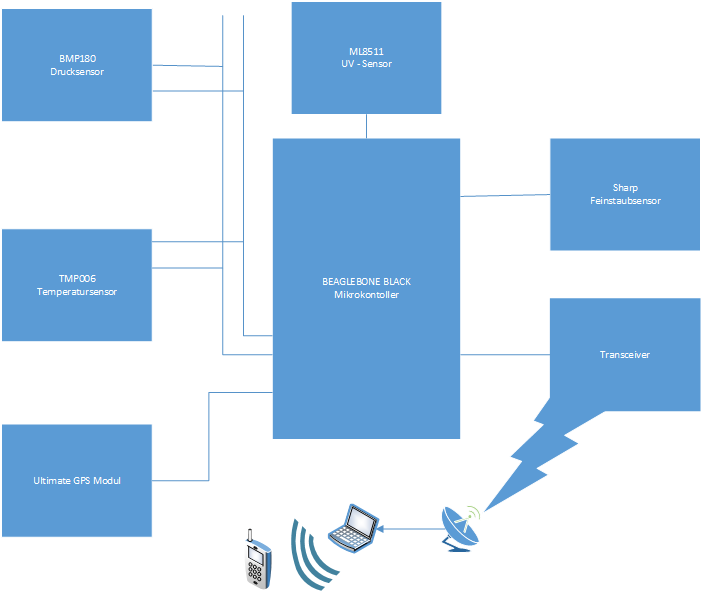
\includegraphics[width=0.8\textwidth]{8_Anhang/Blockdiagramm.png}
	\caption{Blockdiagramm vom CanSat}
	\label{blockdiagramm}
\end{figure}

\newpage

\subsection{GANTT-Diagramme}
\subsubsection {Hardware-GANTT}
\begin{figure}[htbp]
	\centering
	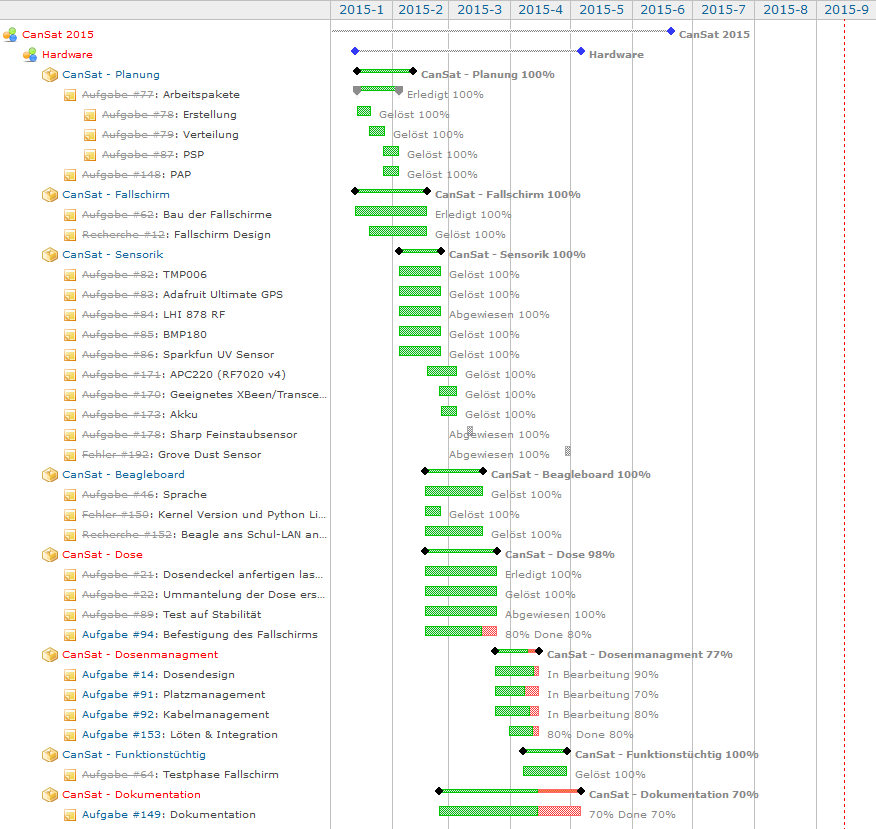
\includegraphics[trim = 2mm 2mm 2mm 2mm, clip,width=0.8\textwidth]{8_Anhang/hardware-gantt-1.png}
	\label{gantt_hardware_1}
\end{figure}
\vspace{-2cm}

\newpage
\subsubsection {Bodenstation-GANTT}
\begin{figure}[H]
	\centering
	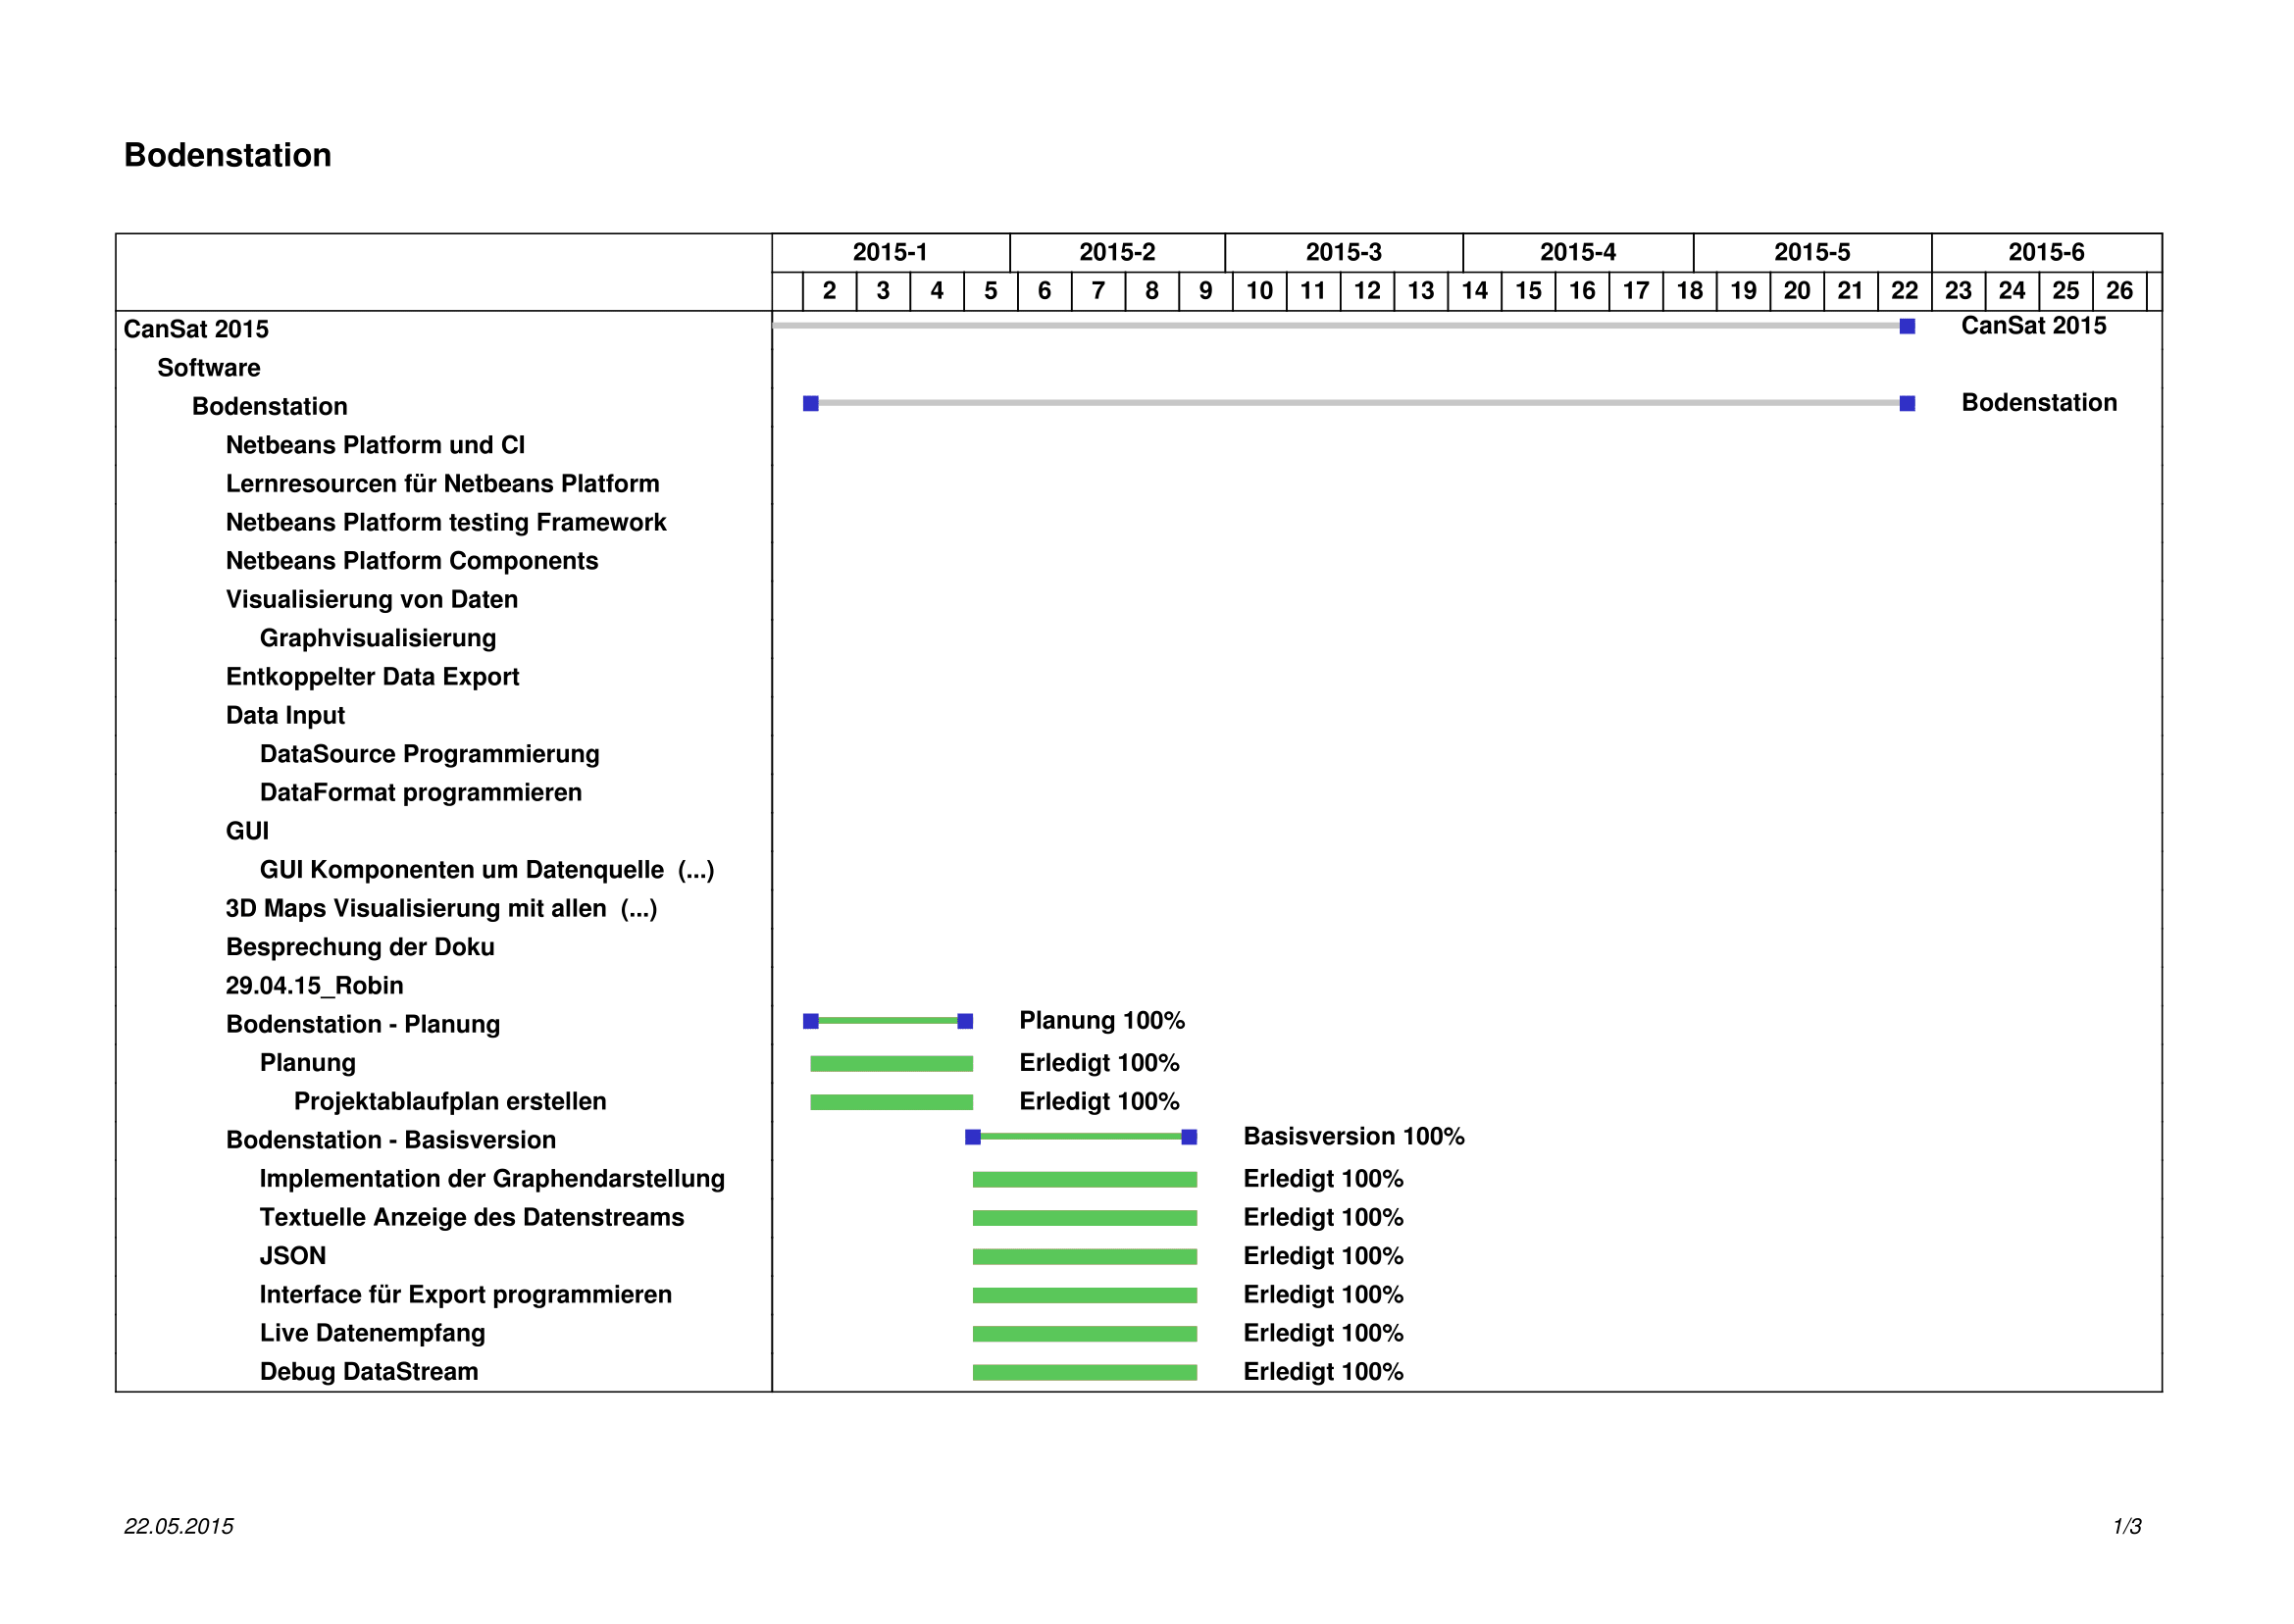
\includegraphics[trim = 25mm 50mm 46mm 65mm, clip,width=0.8\textwidth]{8_Anhang/bodenstation-gantt-1.png}
	\label{gantt_hardware_1}
\end{figure}
\vspace{-1,3cm}
\begin{figure}[H]
	\centering
	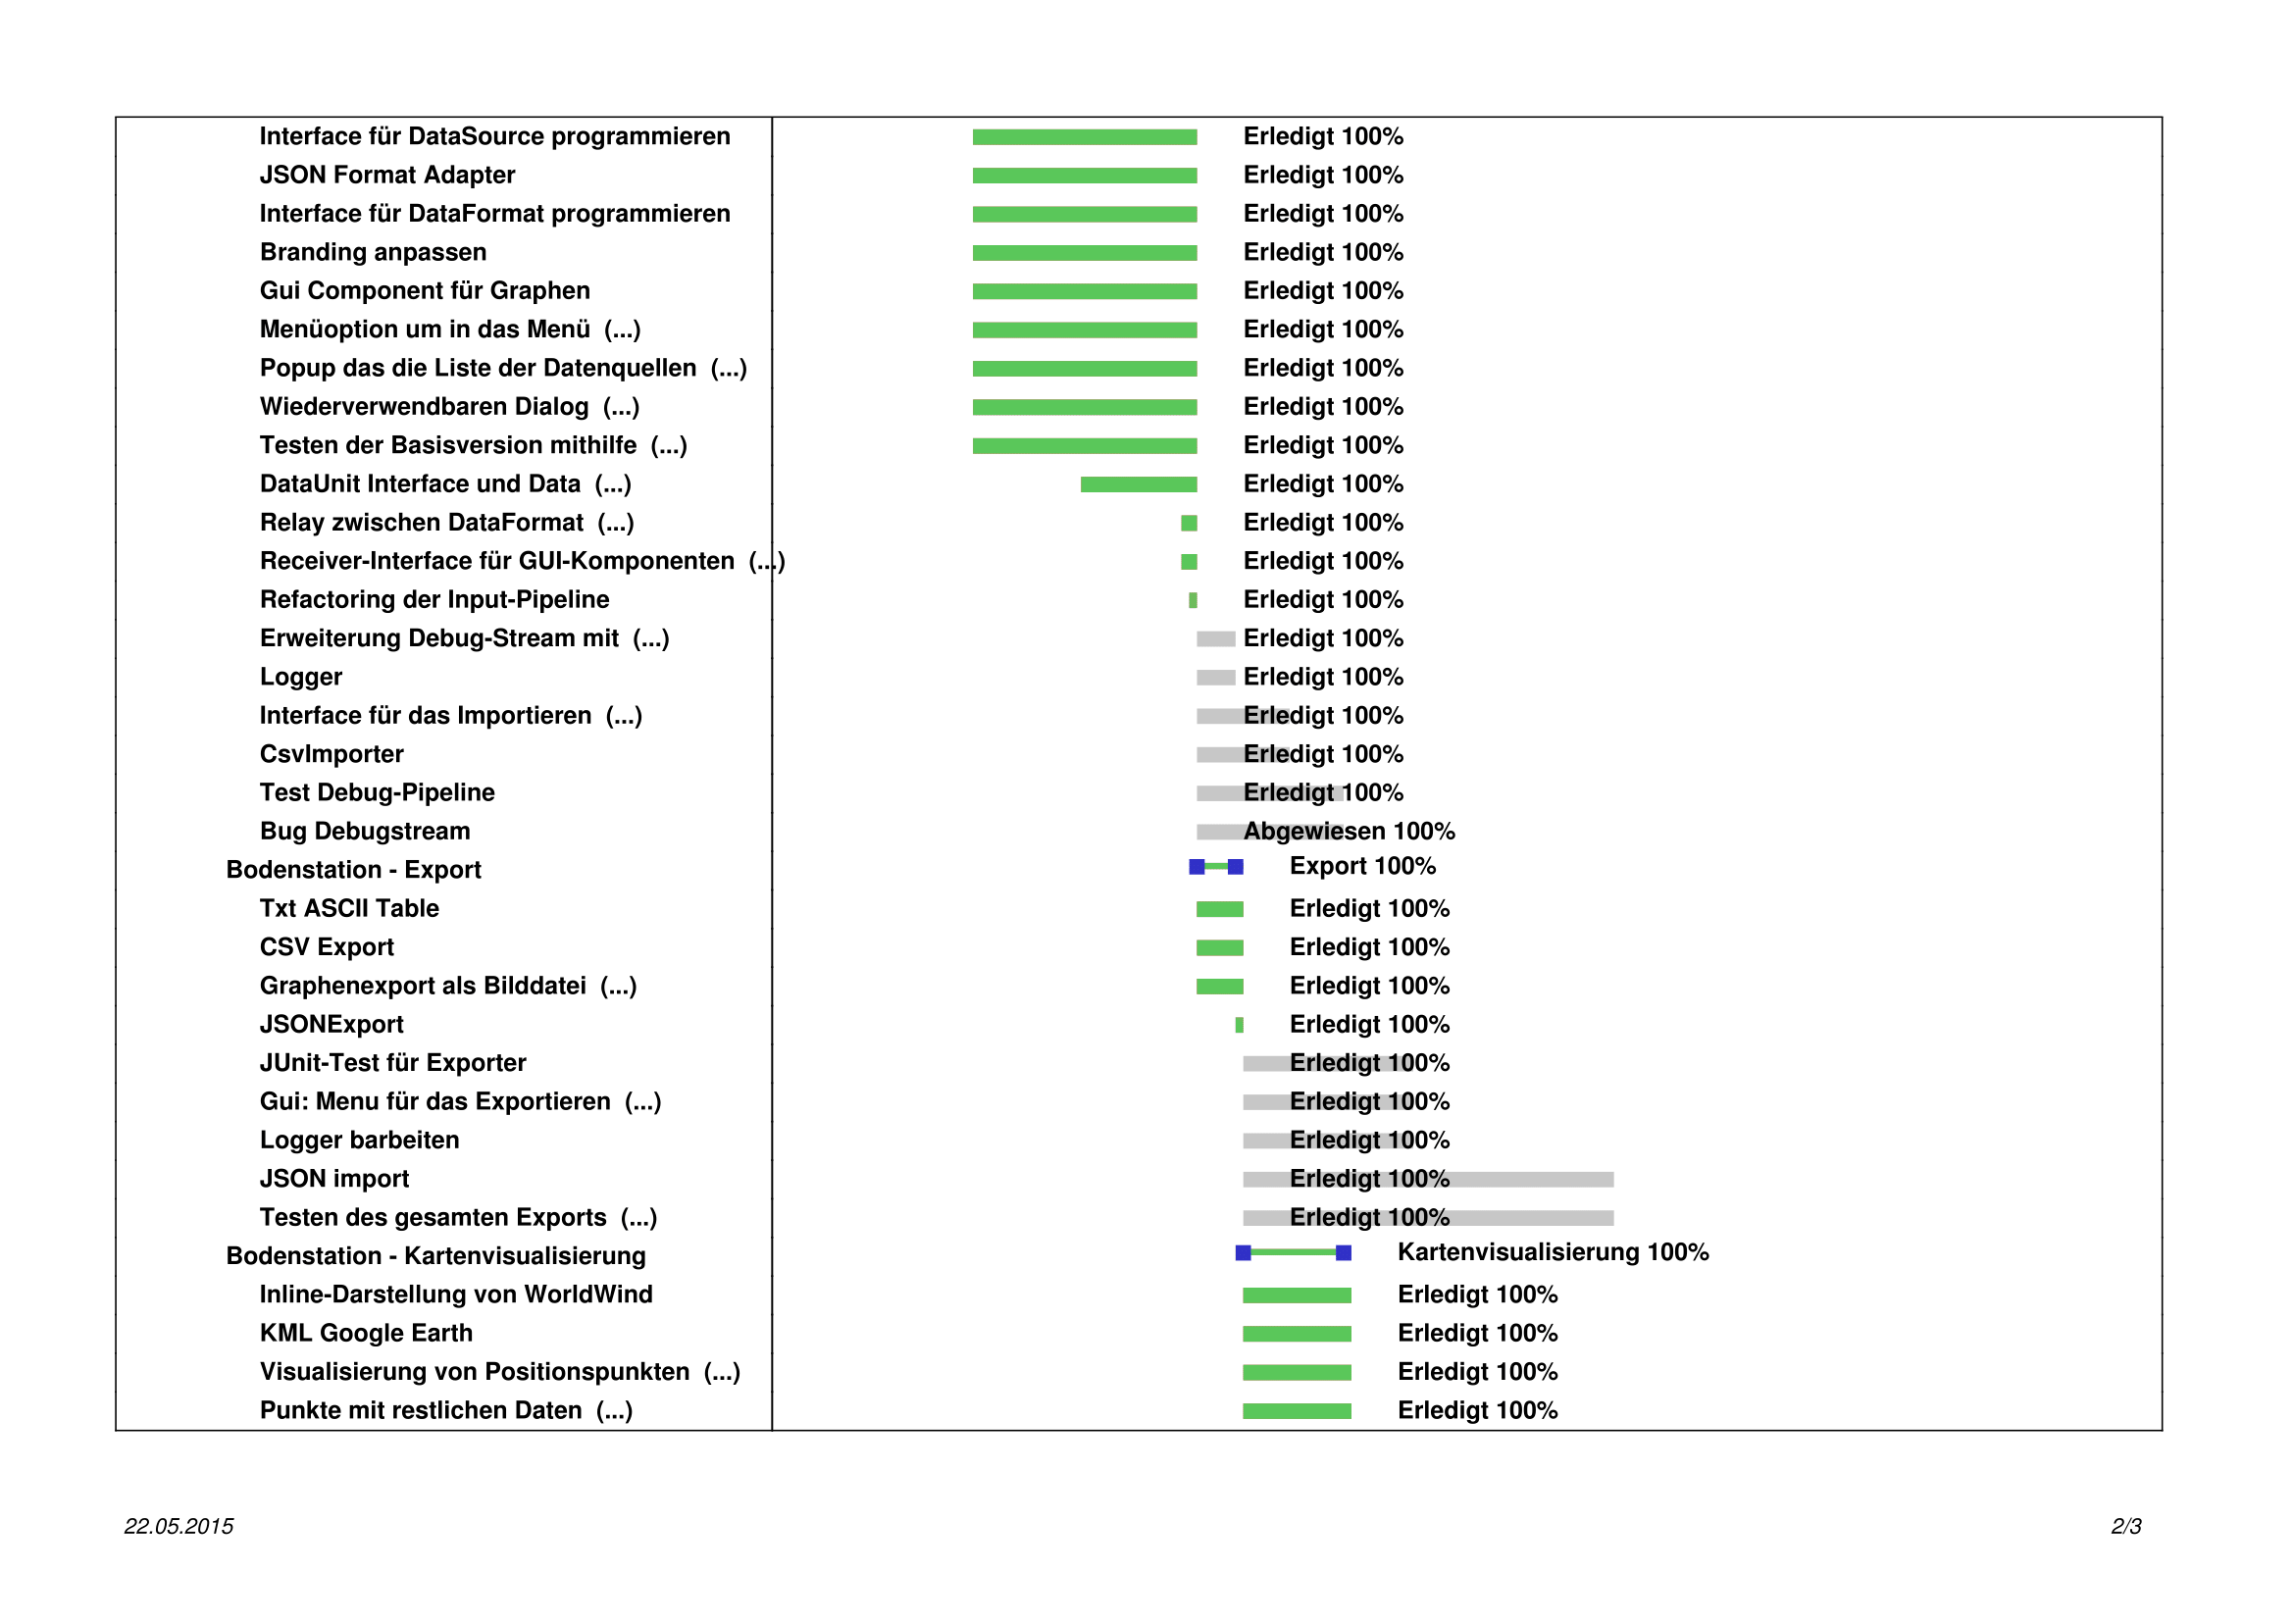
\includegraphics[trim = 30mm 50mm 45mm 40mm, clip,width=0.8\textwidth]{8_Anhang/bodenstation-gantt-2.png}
	\label{gantt_hardware_2}
\end{figure}
\vspace{-1,1cm}
\begin{figure}[H]
	\centering
	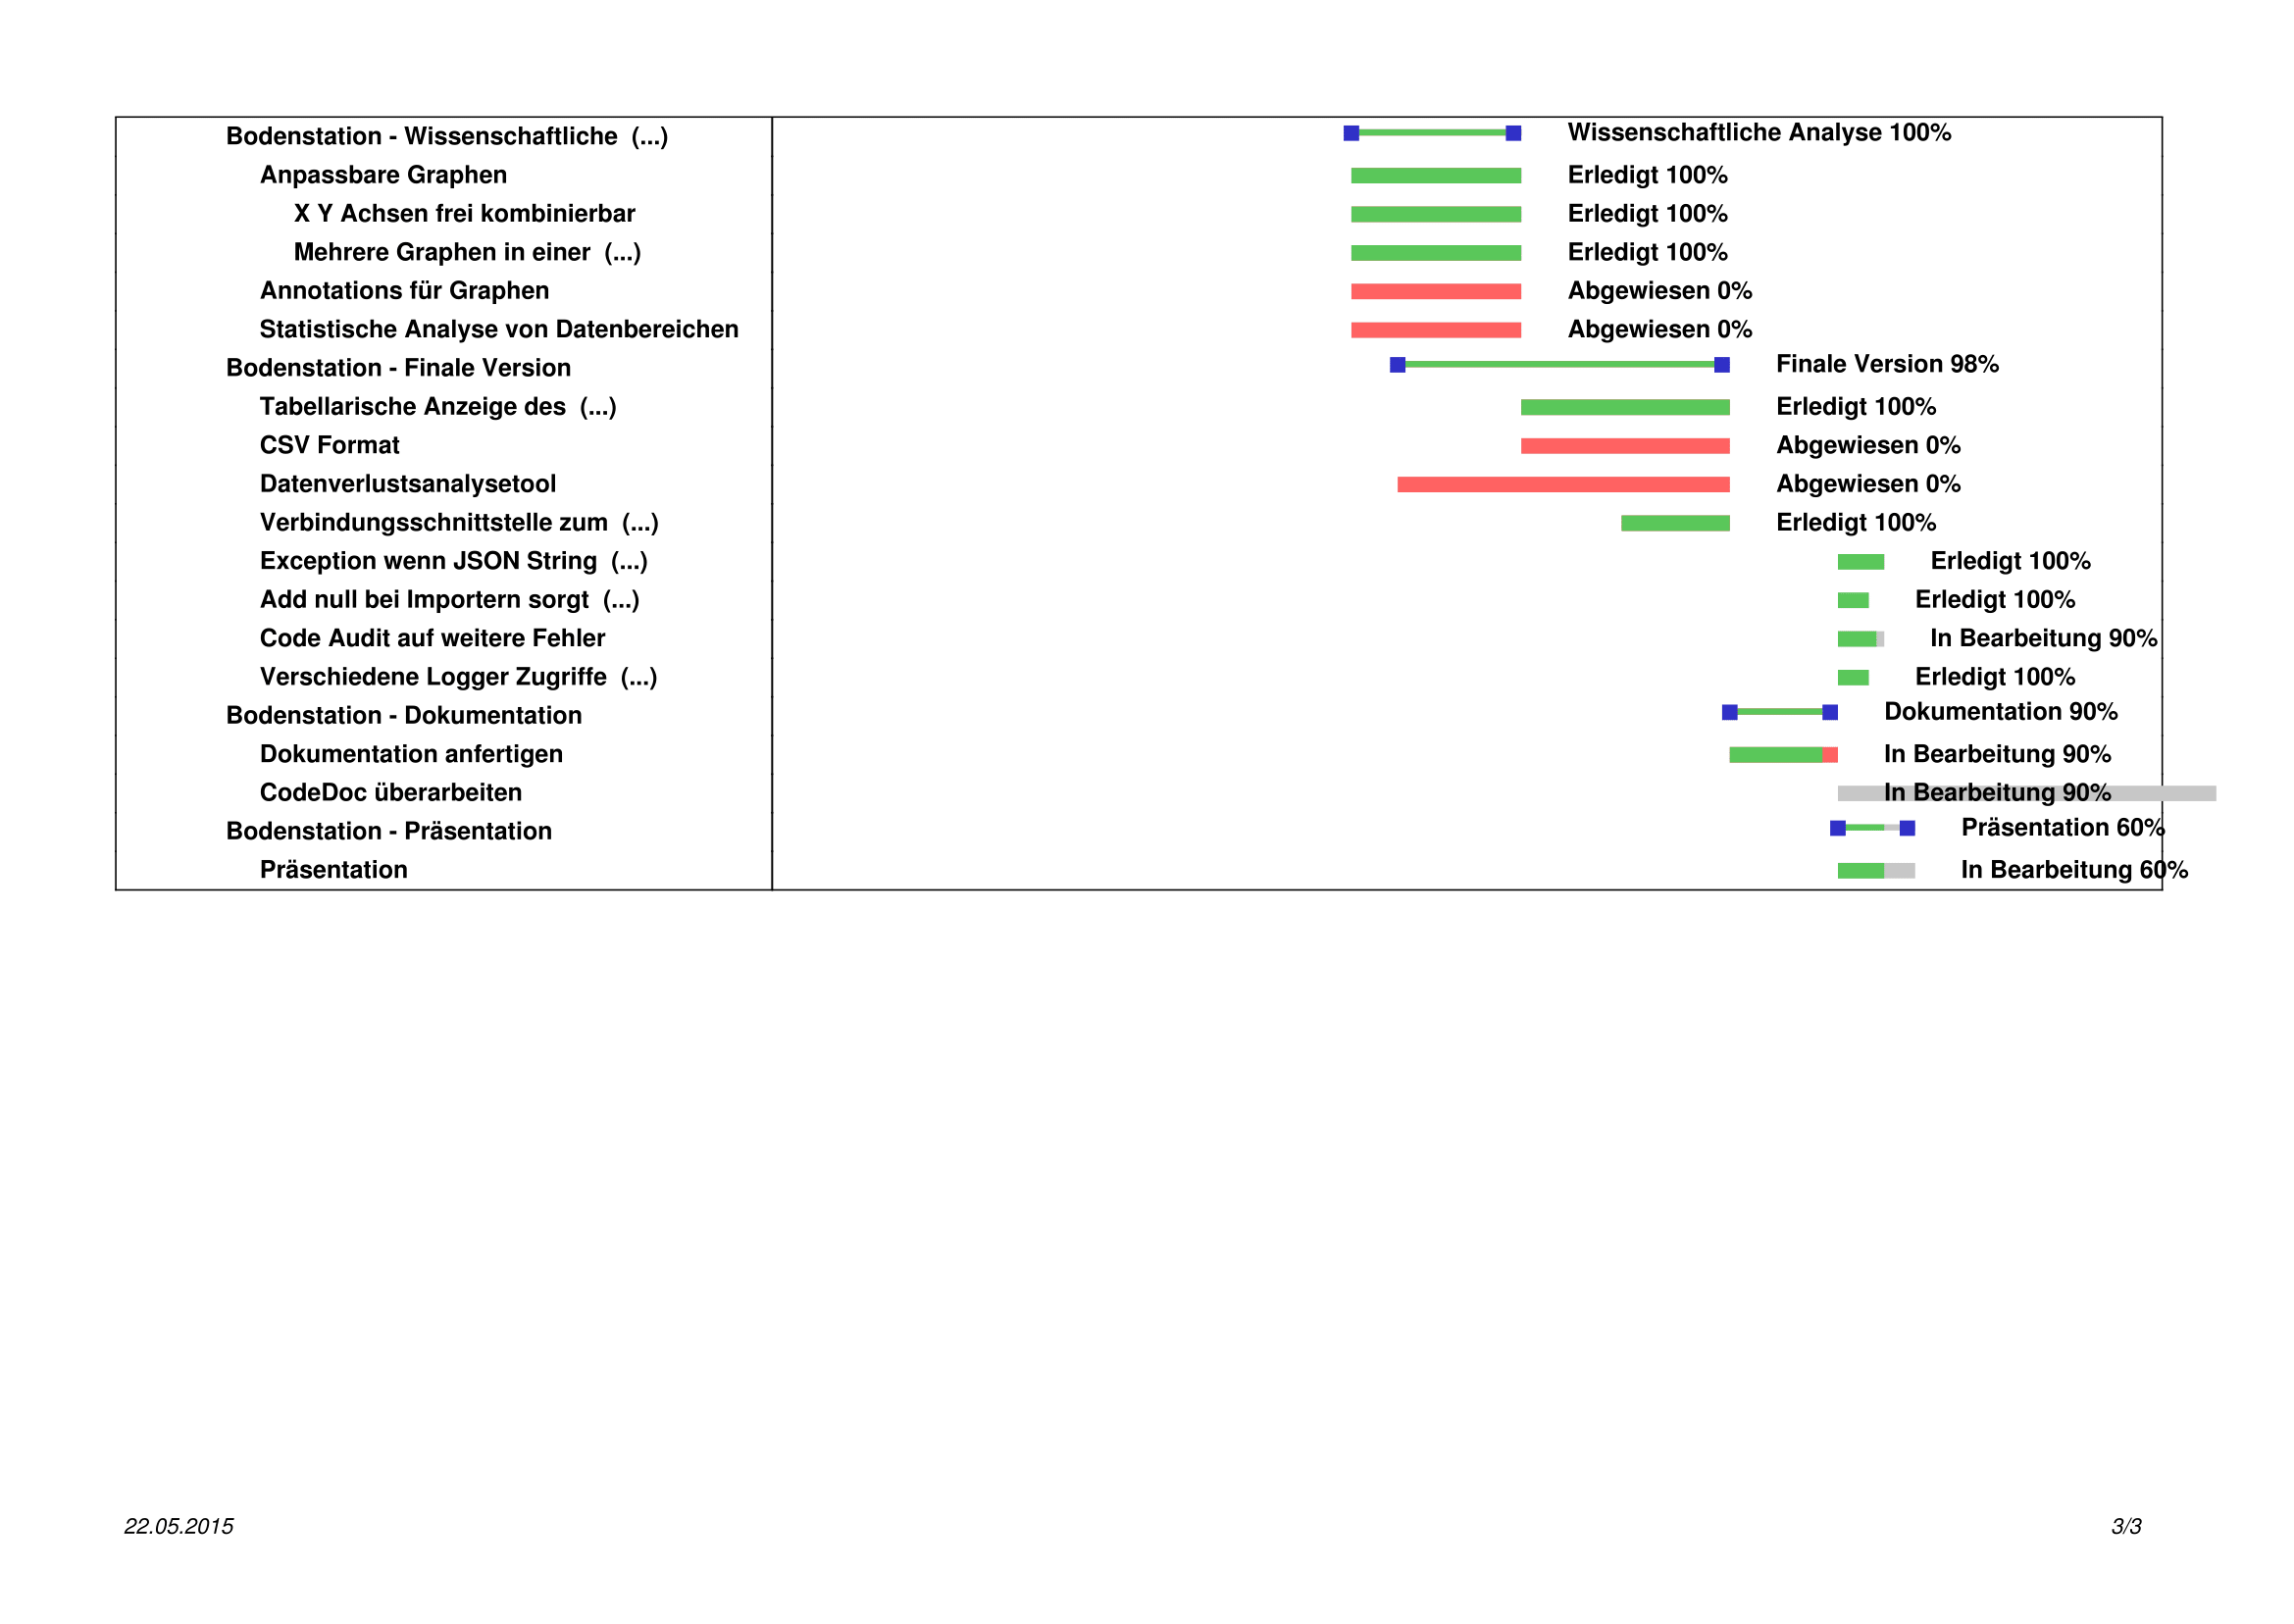
\includegraphics[trim = 30mm 200mm 45mm 40mm, clip,width=0.8\textwidth]{8_Anhang/bodenstation-gantt-3.png}
	\caption{Das GANTT-Diagramm der Bodenstation}
	\label{gantt_hardware_3}
\end{figure}
\newpage
\subsubsection {Android-App-GANTT}
\begin{figure}[H]
	\centering
	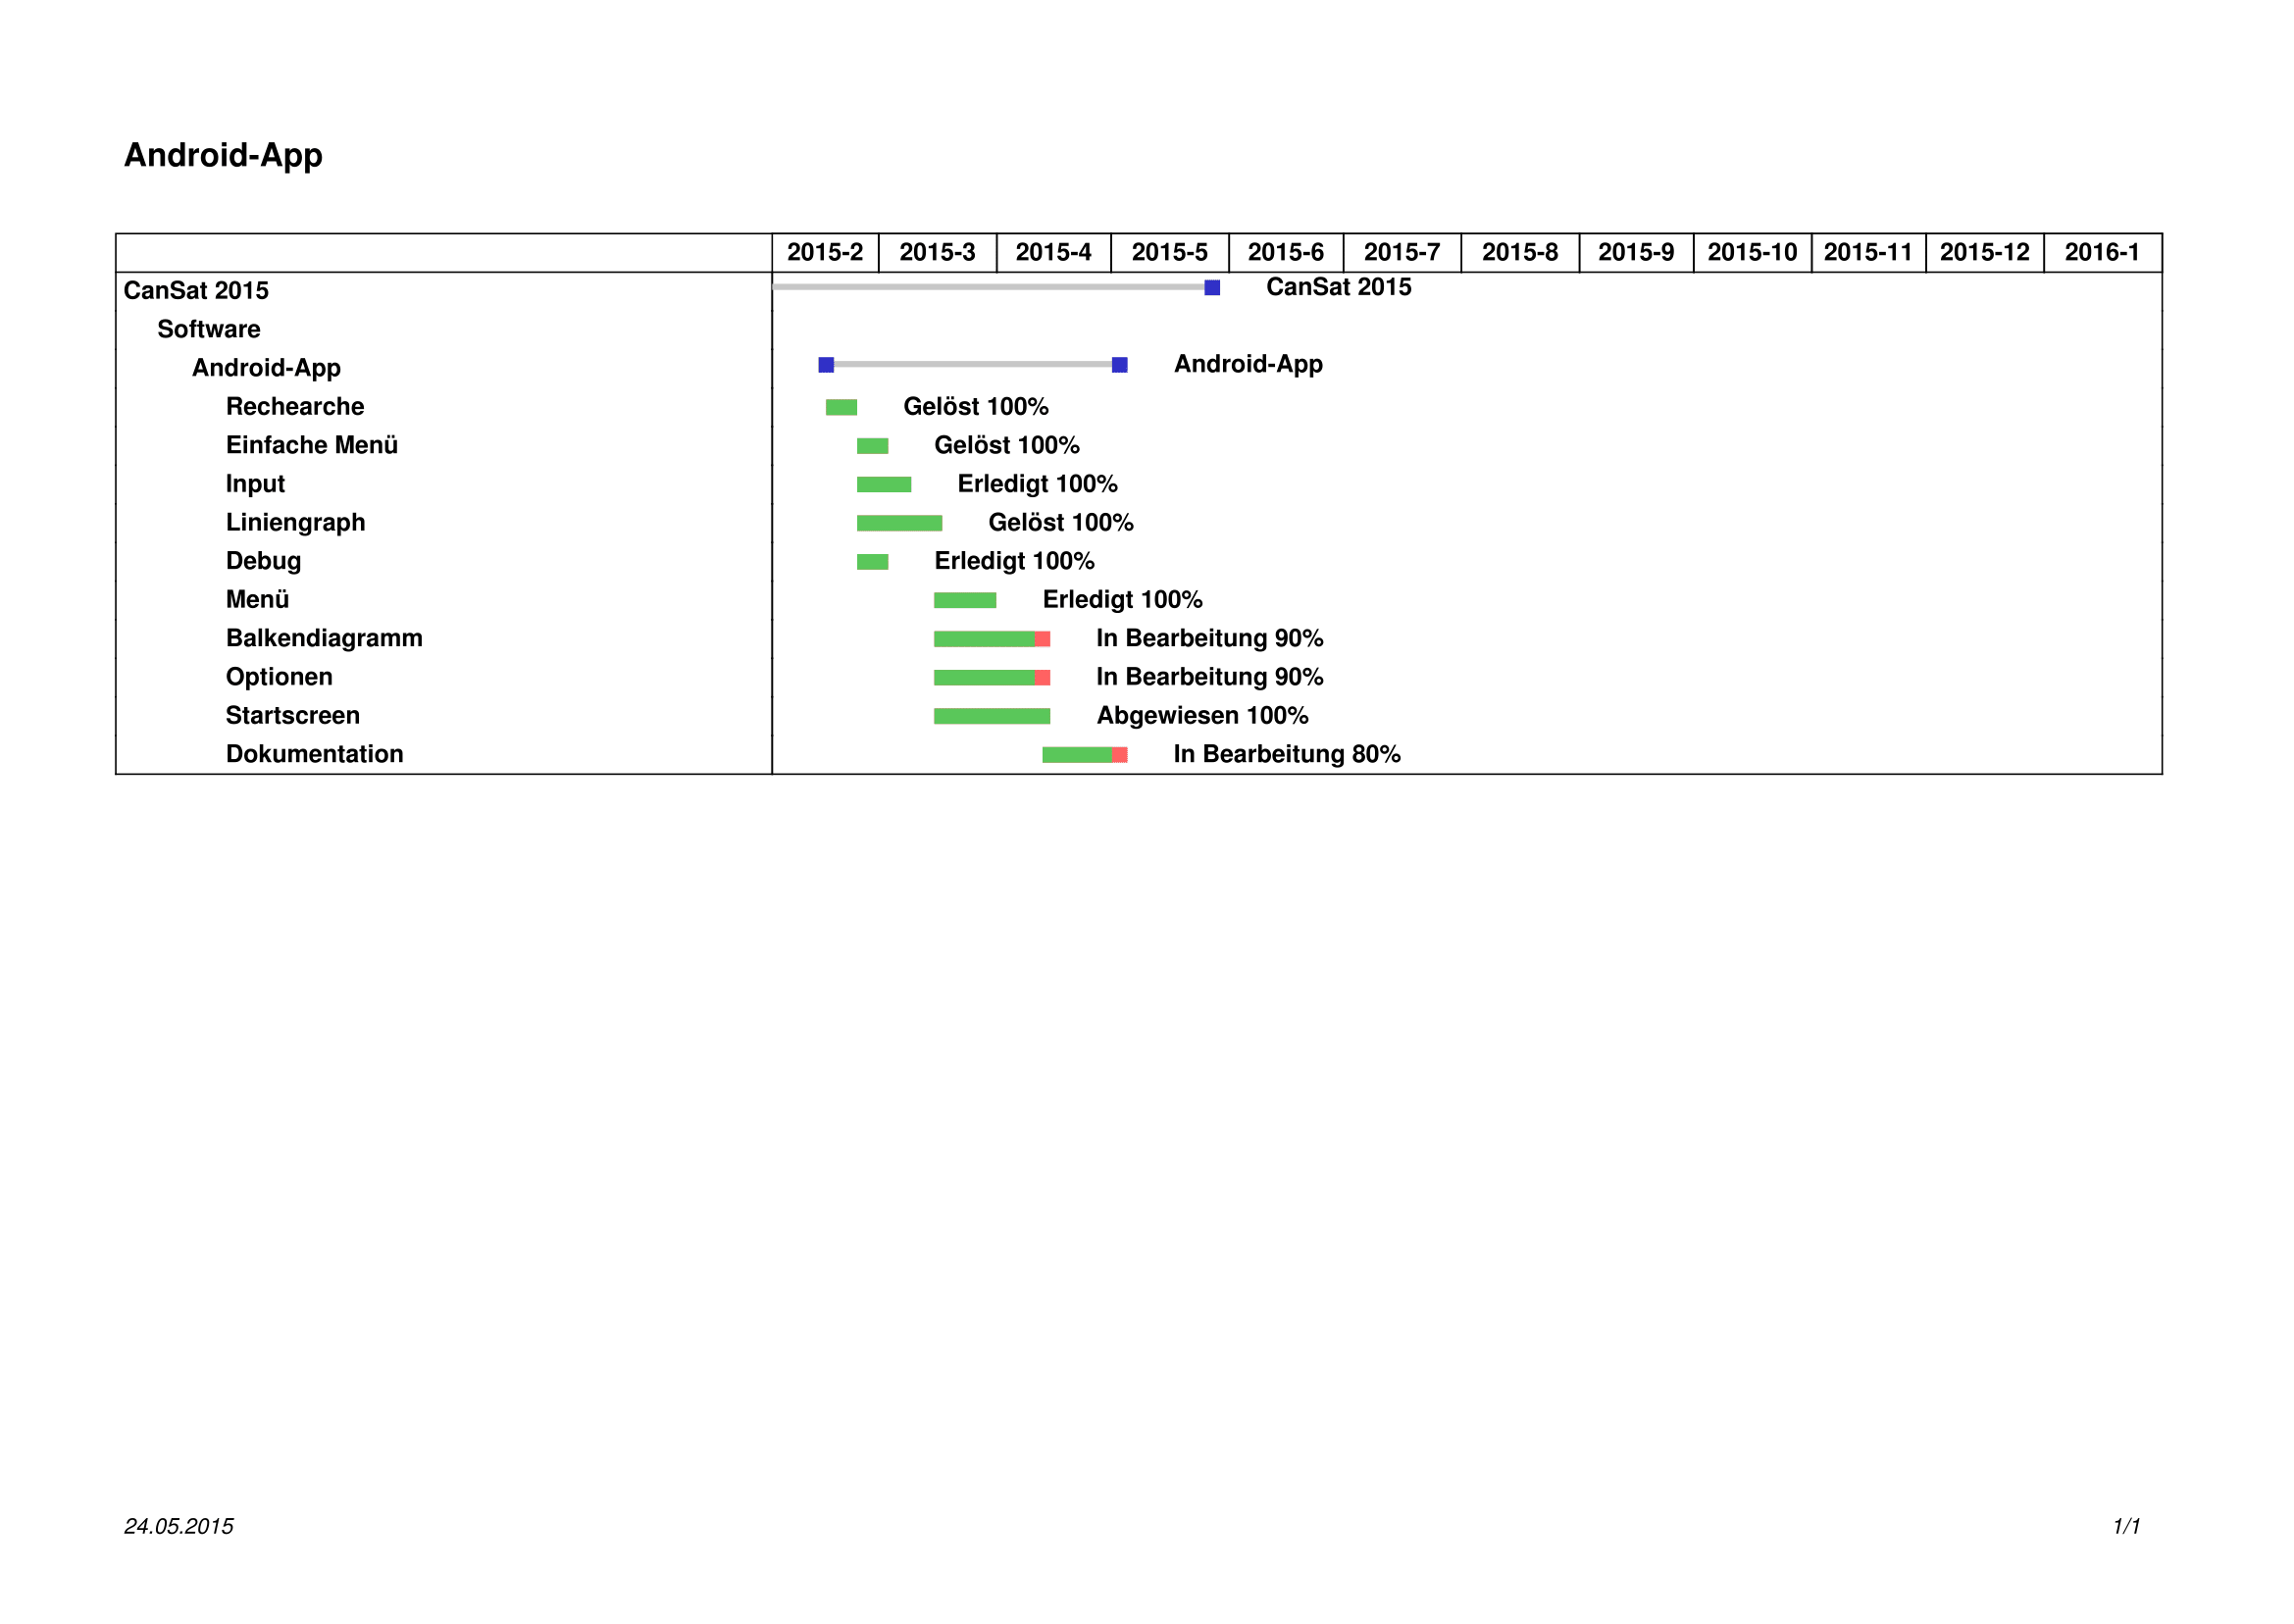
\includegraphics[trim = 30mm 200mm 45mm 40mm, clip,width=0.8\textwidth]{8_Anhang/android-app-gantt.png}
	\caption{Das GANTT-Diagramm der Android-App}
	\label{gantt_hardware_3}
\end{figure}

\newpage
\vspace{-2cm}
\subsection{Der CanSat}

\begin{figure}[H]
	\centering
	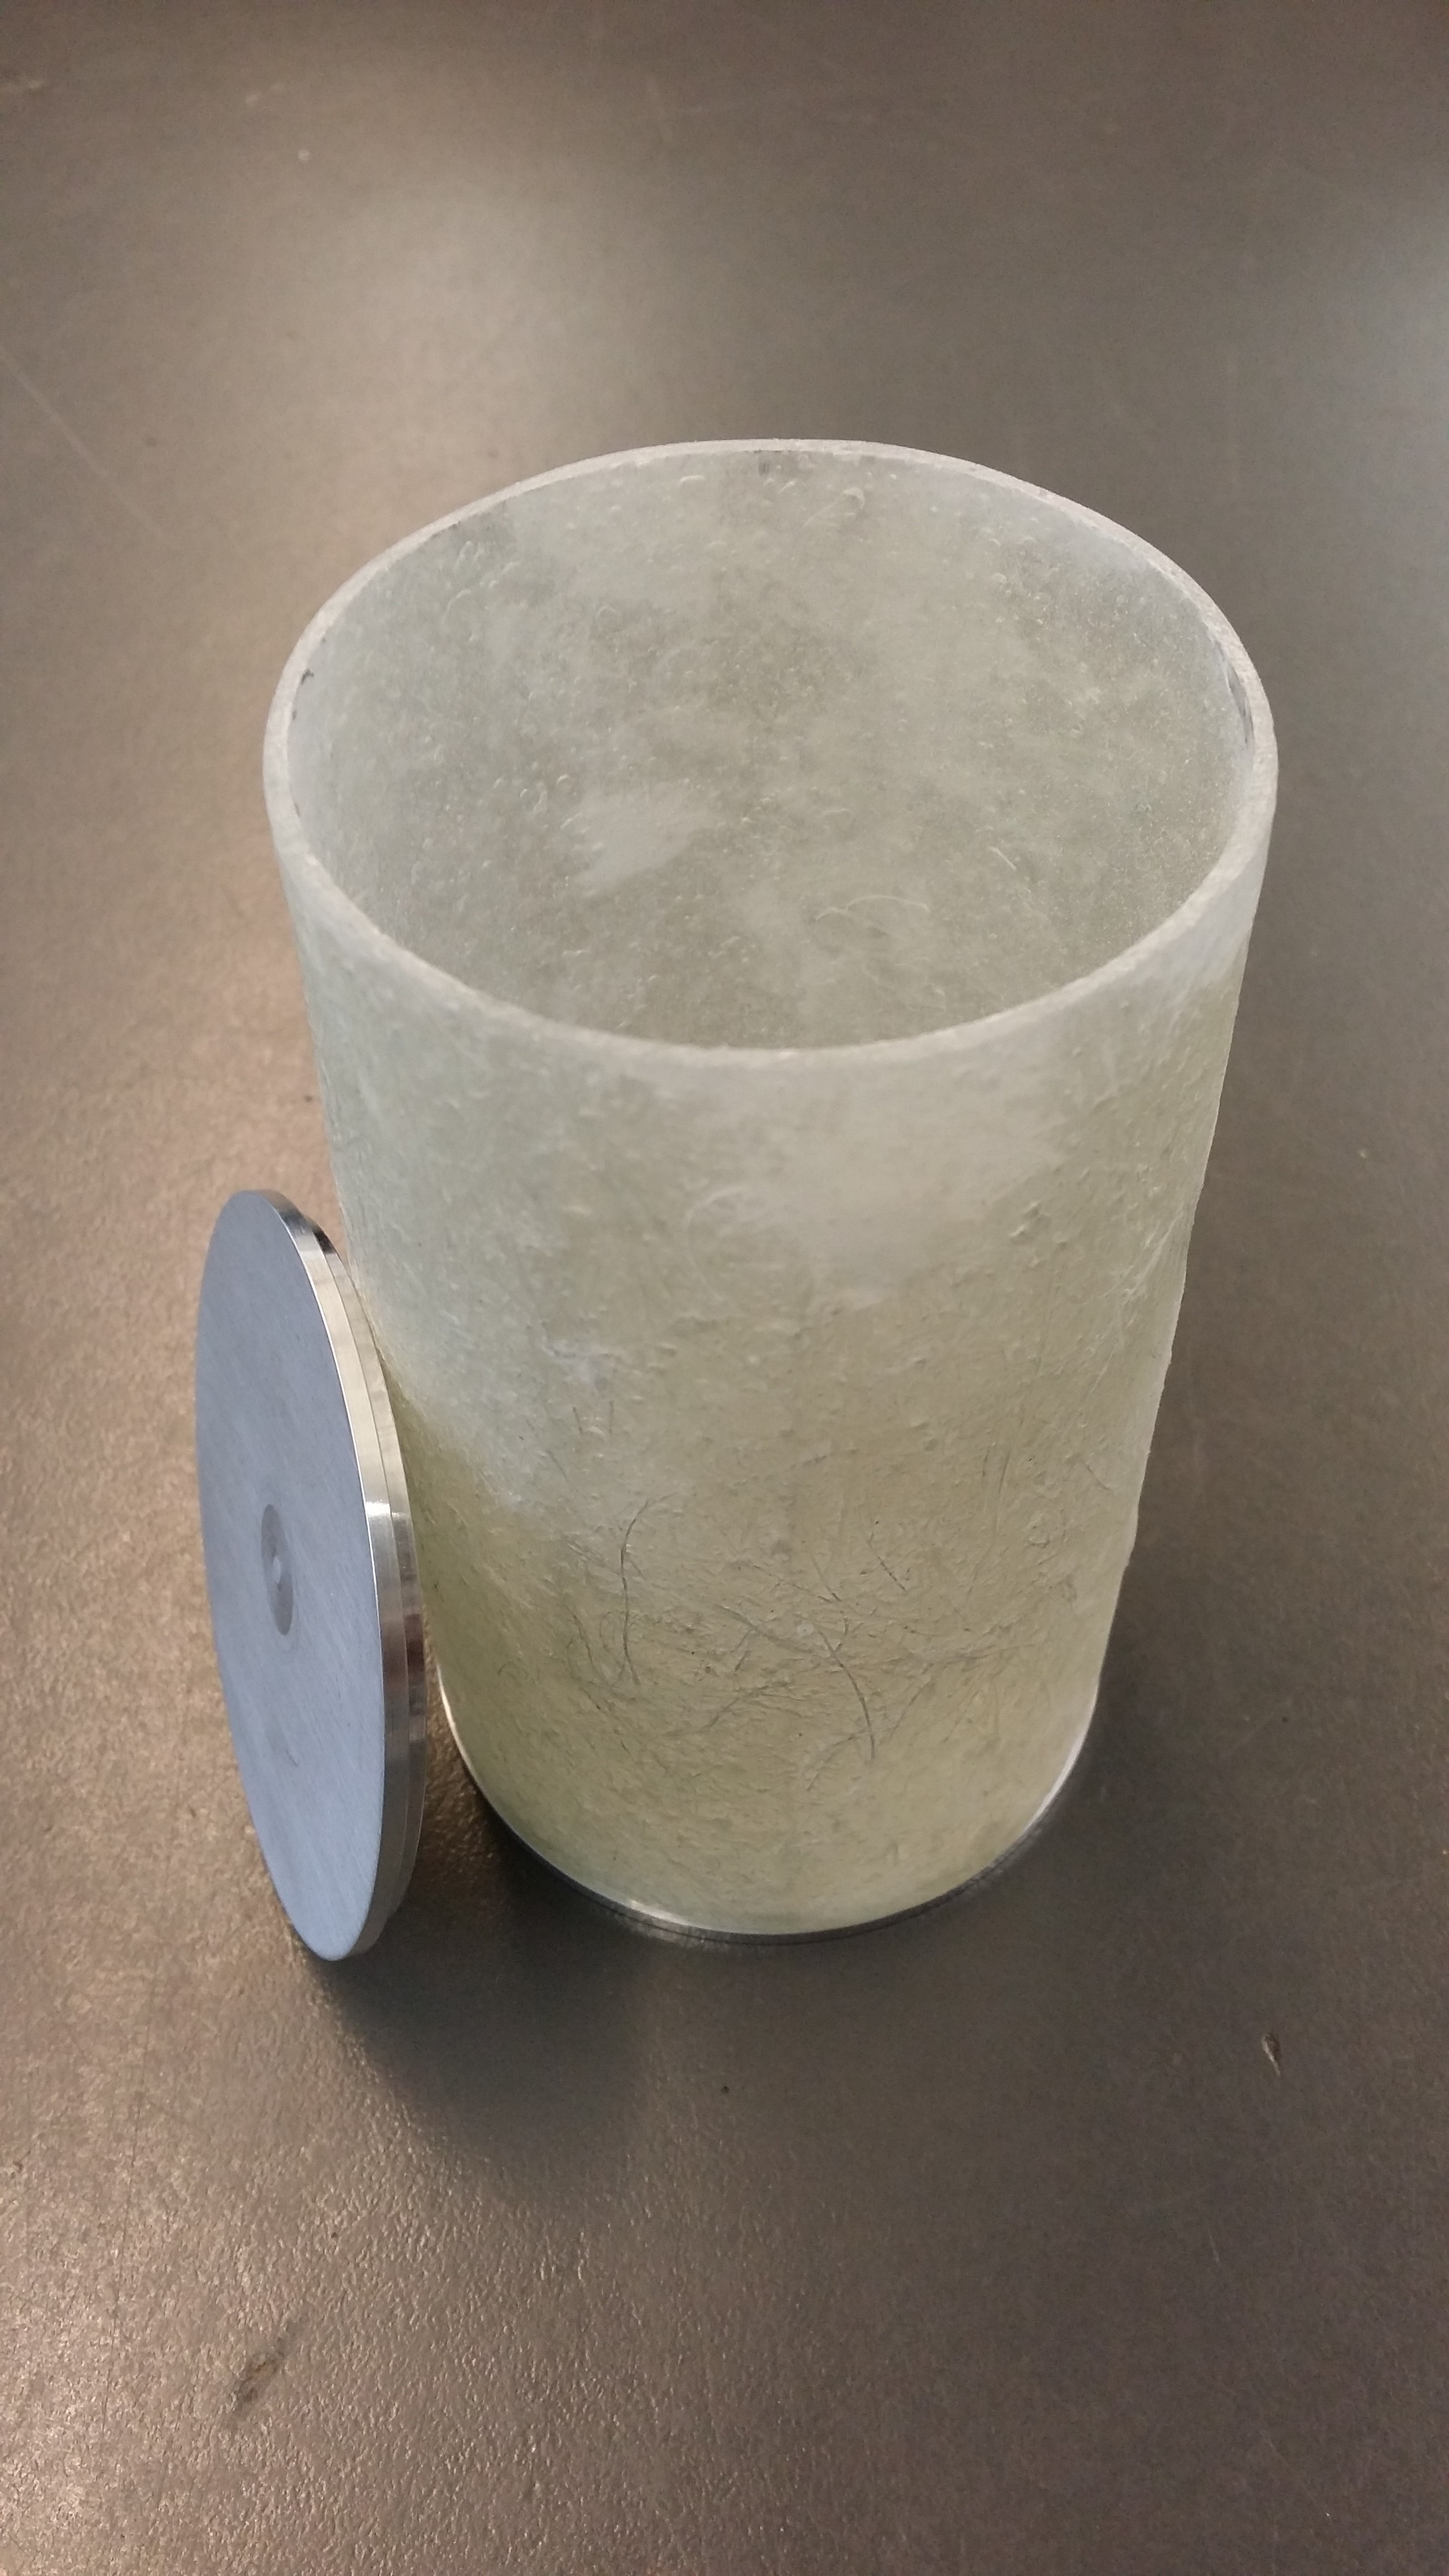
\includegraphics[trim = 11mm 335mm 20mm 210mm, clip, width=0.8\textwidth]{8_Anhang/dose.jpg}
	\caption{Die Hülle und ein Dosendeckel}
	\label{pic_dose}
\end{figure}

\begin{figure}[H]
	\centering
	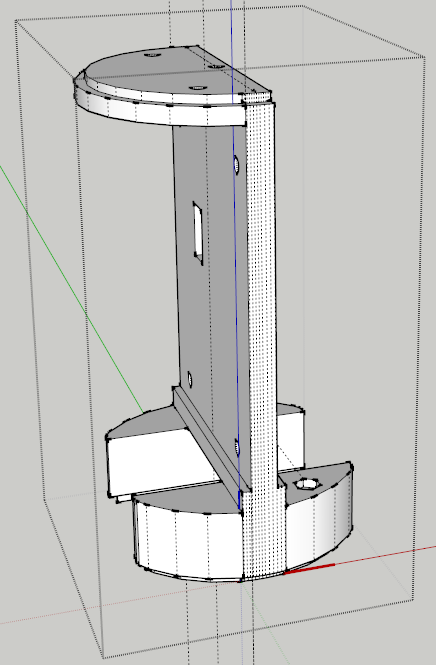
\includegraphics[ width=0.8\textwidth]{8_Anhang/Wand_3D.PNG}
	\caption{Screenshot der Zwischenwand aus Sketchup}
	\label{pic_wand_3d}
\end{figure}

\newpage

\begin{figure}[h] 
      \centering 
      \includemovie[ 
        poster,controls,
       3Djscript=2_Beschreibung_des_CANSAT/Encompass.js
      ]{0.8\textwidth}{15cm}{2_Beschreibung_des_CANSAT/CanSat_2015.u3d} 
      \caption{Der Satellit (Diese Zeichnung ist möglicherweiße nicht sichtbar, da es eine 3D-Zeichnung ist. Bitte verwenden Sie den \href{https://get.adobe.com/reader/?loc=de}{Adobe Acrobat Reader})}\label{pic_3d} 
\end{figure} 

\newpage

\begin{figure}[H]
	\centering
	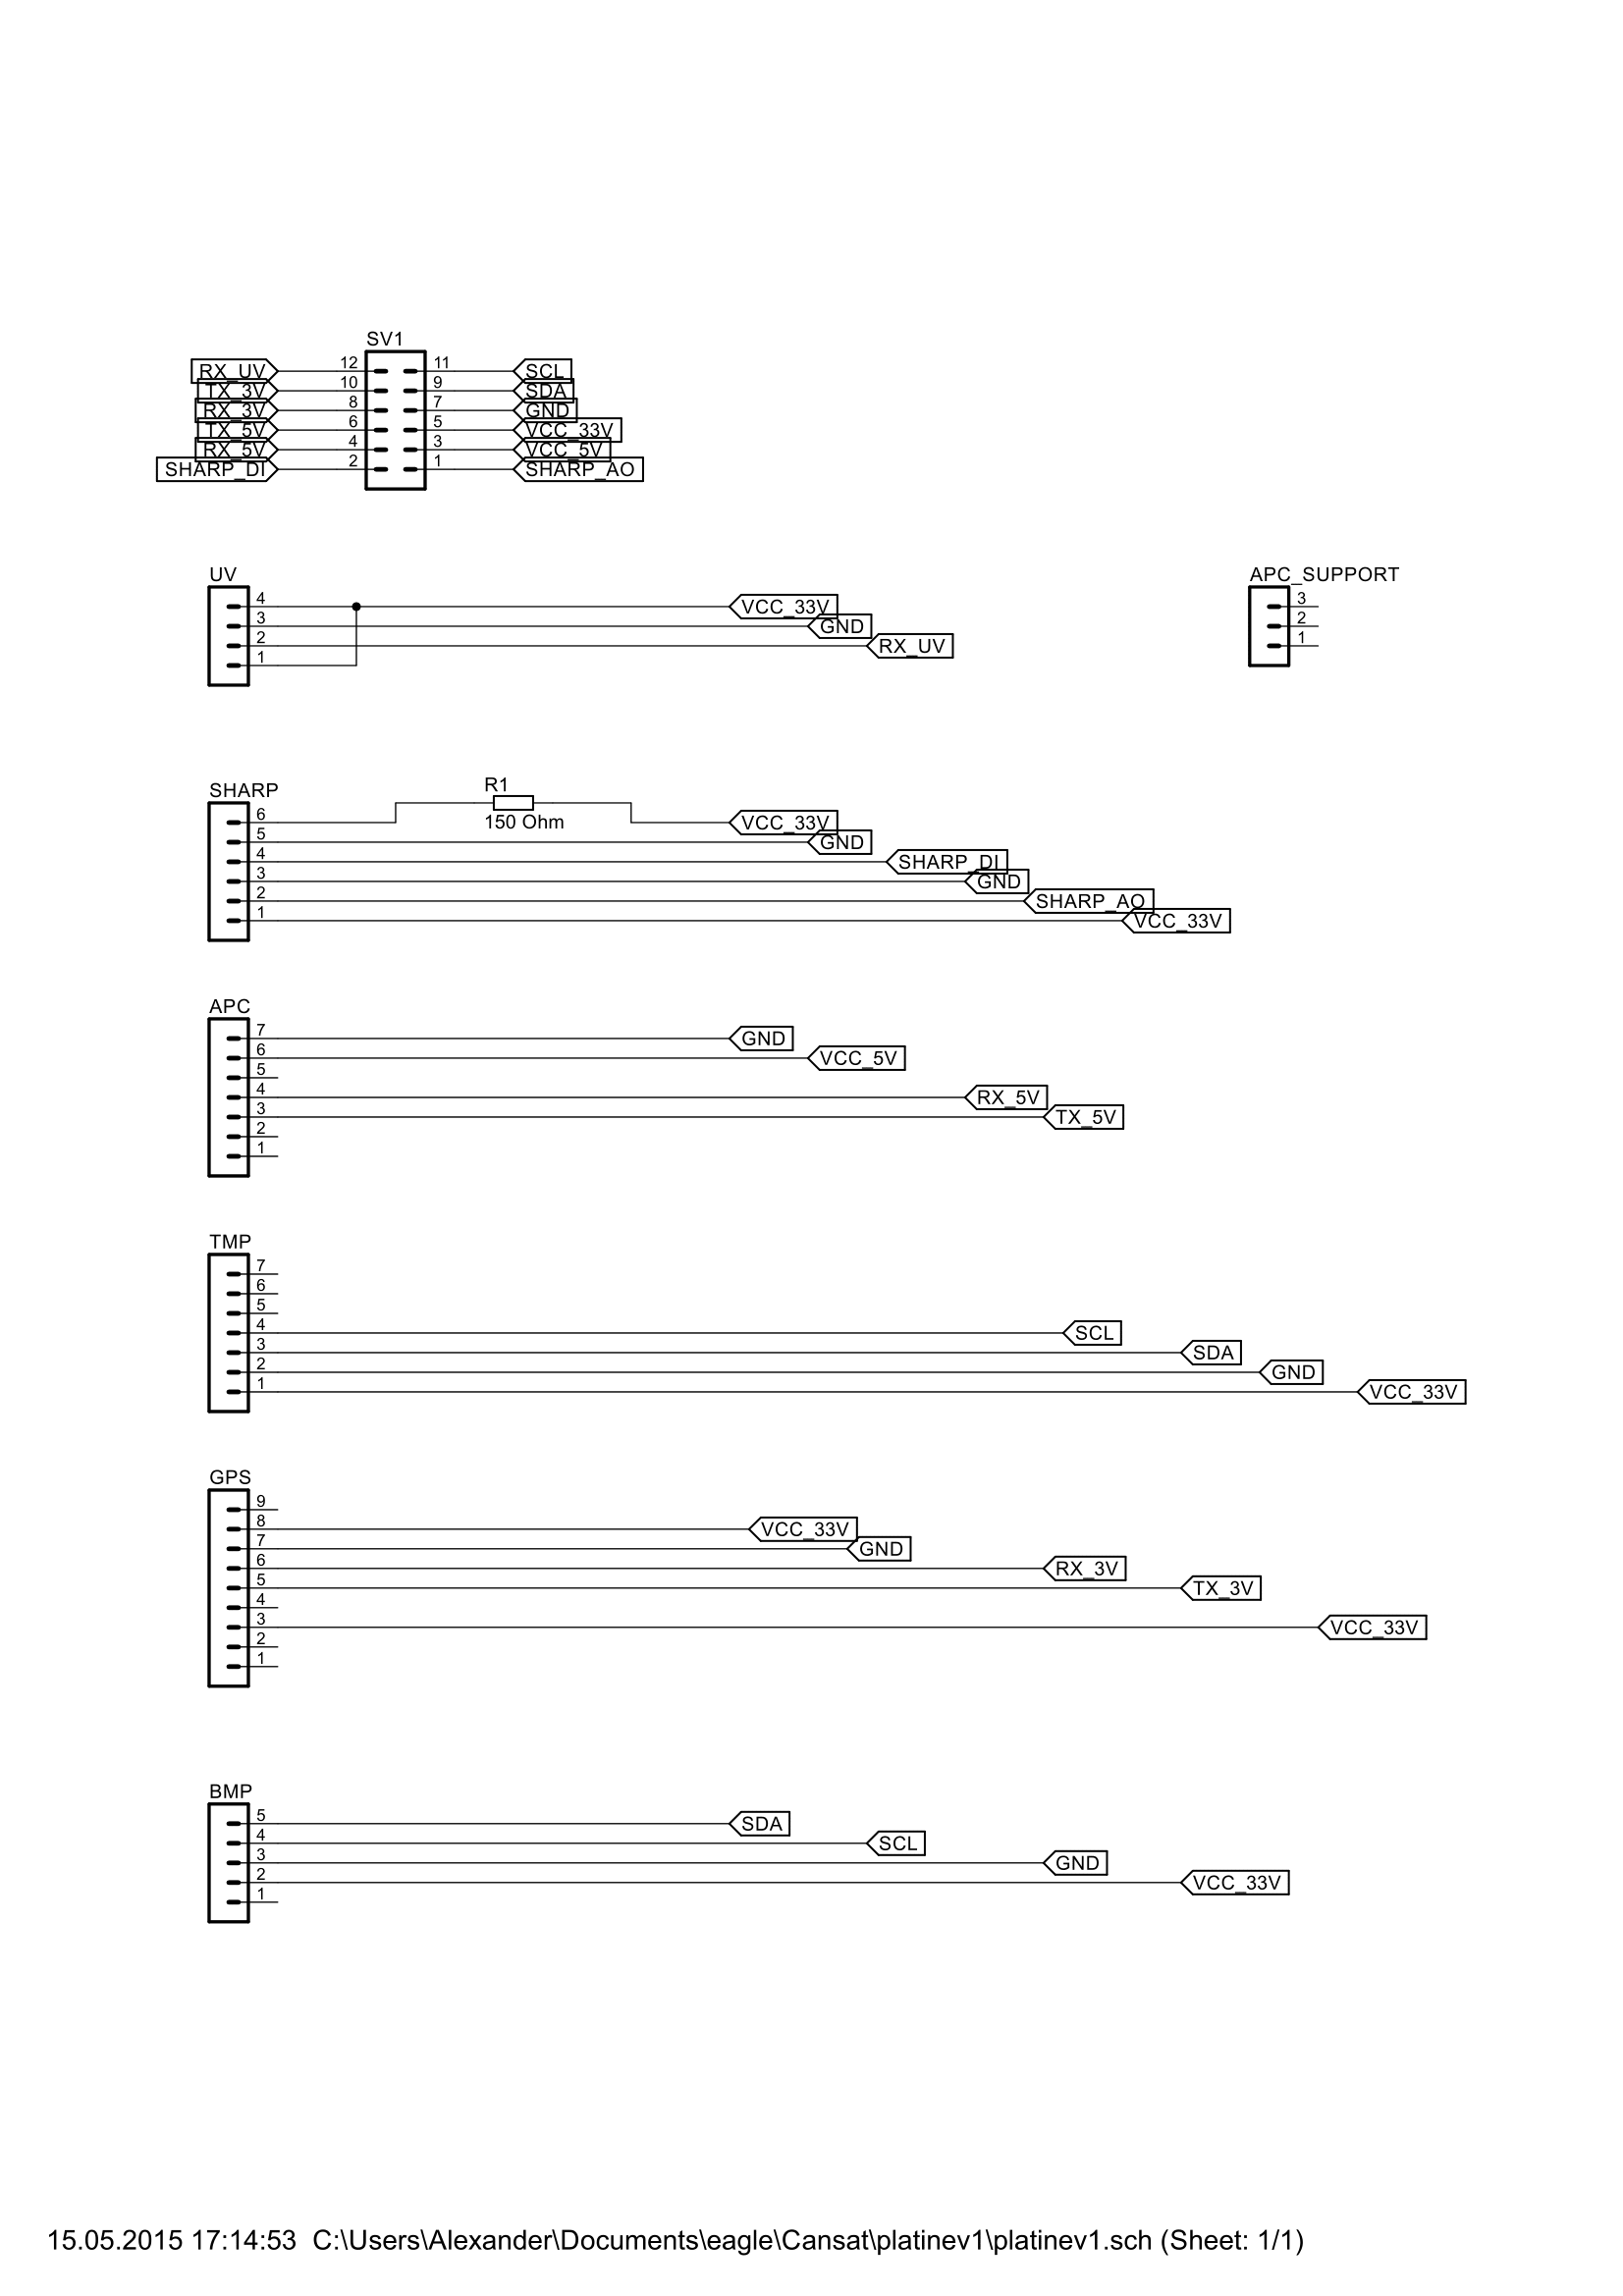
\includegraphics[trim = 60mm 100mm 55mm 100mm, clip, width=0.8\textwidth]{8_Anhang/Schaltplanv1.png}
	\caption{Der Schaltplan der Sensorikplatine}
	\label{pic_schaltplan}
\end{figure}

\newpage

\begin{figure}[H]
	\centering
	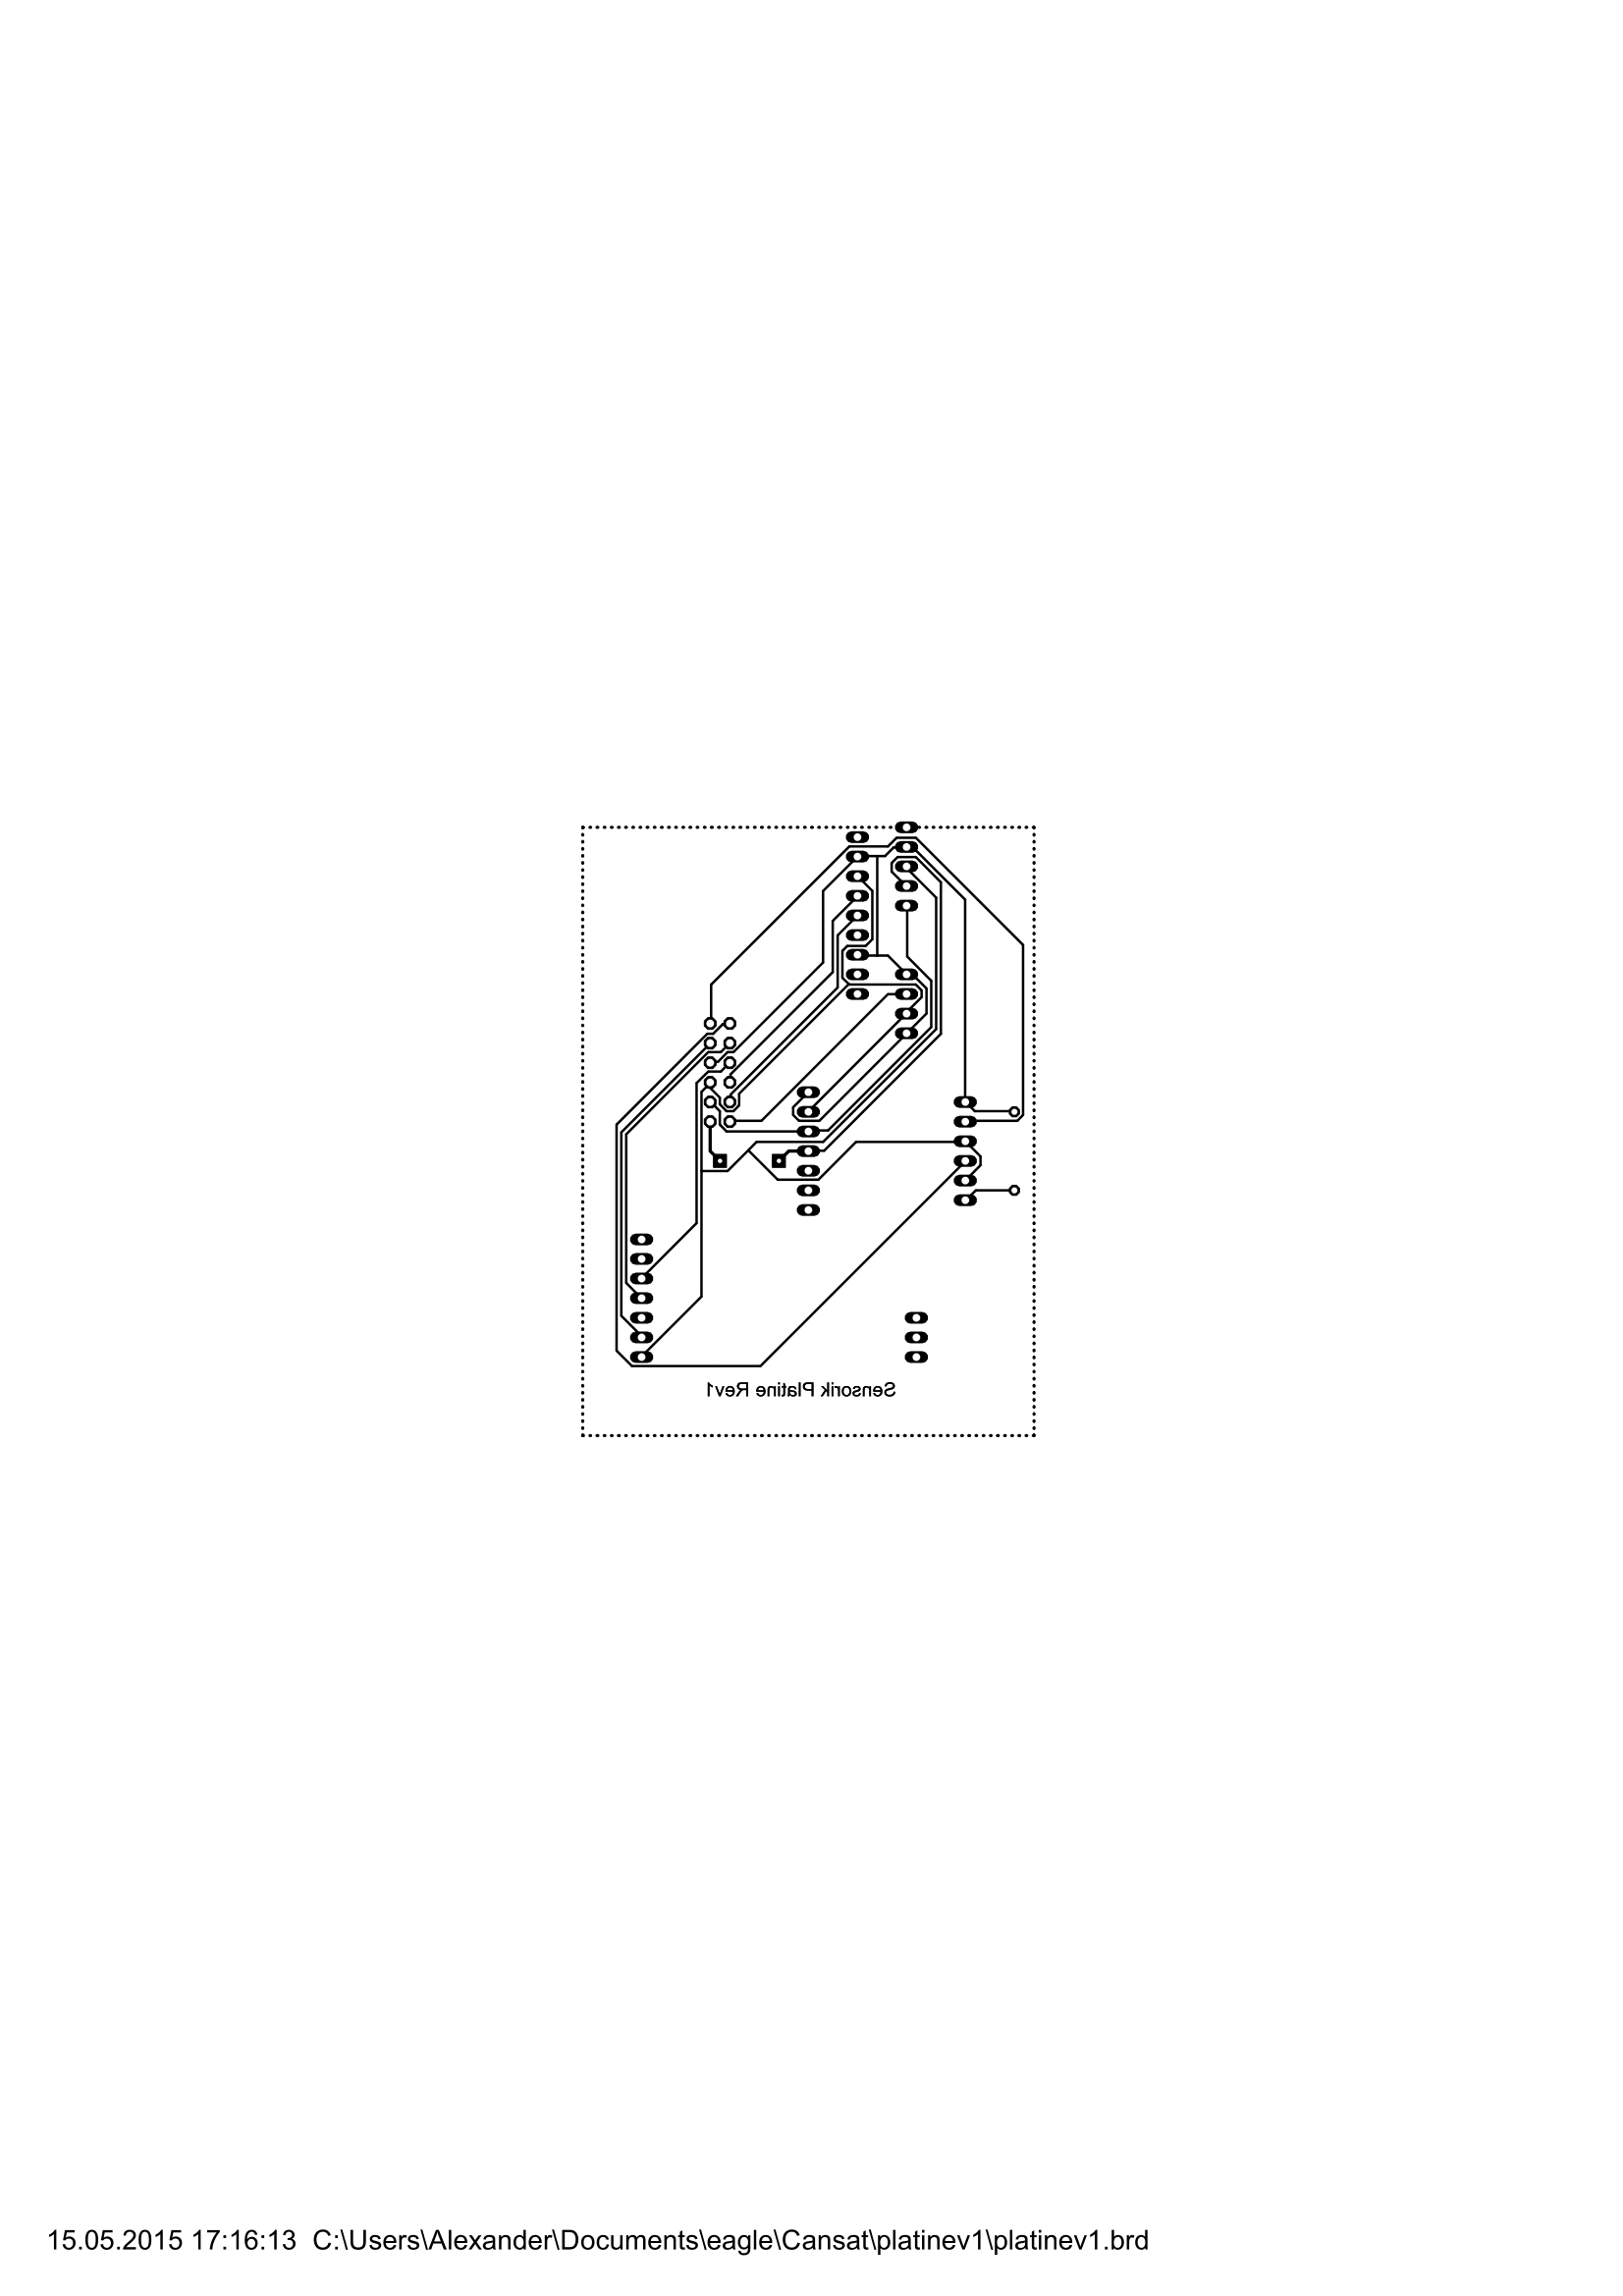
\includegraphics[trim = 200mm 300mm 200mm 280mm, clip,width=0.8\textwidth]{8_Anhang/Layoutv1.png}
	\caption{Das Layout der Sensorikplatine}
	\label{pic_layout}
\end{figure}

\newpage

\begin{figure}[H]
	\centering
	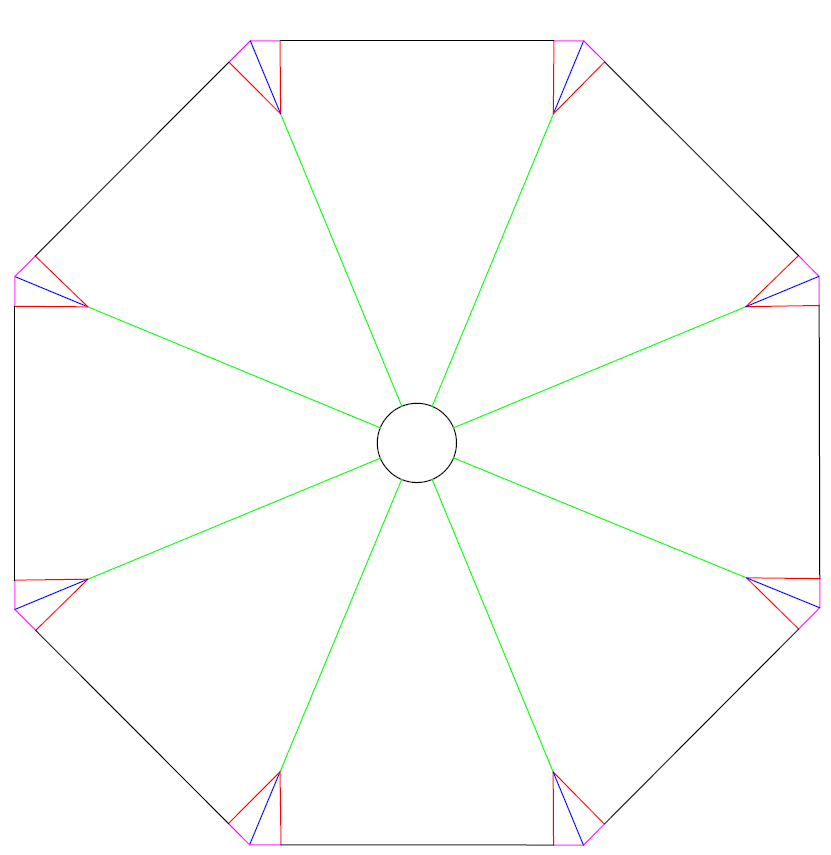
\includegraphics[ width=0.8\textwidth]{8_Anhang/fallschirmSkizze.PNG}
	\caption{Skizze des Fallschirms}
	\label{pic_fallschrimskizze}
\end{figure}

\newpage

\subsection{Bodenstationsnutzeranleitung}
\subsubsection{Nutzeranleitung}
Die hier vorgestellte Nutzeranleitung repräsentiert die Nutzeranleitung des Produktes, wenn es komplett fertiggestellt ist. \\
Da dies noch nicht komplett der Fall ist, kann es Abweichungen zwischen der Nutzeranleitung und dem für das P5 abgegebene Produkt geben.

\paragraph{Datenempfang}
Um Daten in Echtzeit zu empfangen, muss eine Verbindung zu einem Satelliten aufgebaut werden. Hierzu muss generell zu allererst ein Satellit erstellt werden. Hierfür wählt man unter dem Menüpunkt ``File'' den Unterpunkt ``Satellites'' aus. Dort ist es möglich, unter ``Add'', einen Satelliten hinzuzufügen. Um eine Satelliten zu laden, wählt man im selben Unterpunkt ``Manage'' aus. Dort wählt man den Satelliten aus, von welchem man Daten empfangen will. Möchte man den Datenempfangen beginnen, dann klickt man auf das ``Start''-Icon in der Toolbar, was die Datenübertragung startet. Ab hier können verschiedene Visualisierungen geöffnet werden, um die empfangenen Daten darzustellen.
\paragraph{Datenimport}
Um Daten aus einer Datei zu importieren, wird im Menüpunkt ``File'' der Untermenüpunkt ``Import'' ausgewählt. Anschließend wird eine Datei ausgewählt, welche importiert werden soll. Mit der Bestätigung werden die Daten dieser Datei eingelesen.
\paragraph{Datenexport}
Für das Exportieren der Daten gilt, dass alle aktuell geladenen Daten exportiert werden. Darunter fallen entweder zwischengespeicherte Daten einer Liveübertragung, oder Daten, welche aus einer Datei importiert werden.
Zum Exportieren der Daten wird im Menüpunkt ``File'' der Untermenüpunkt ``Export'' ausgewählt. Unter diesem Menüpunkt ist das Datenformat wählbar, in welches die gesammelten Daten gespeichert werden. Anschließend ist ein Pfad und ein Name wählbar, unter dem die Datei gespeichert wird. Mit der Bestätigung werden die Daten exportiert.
\paragraph{Datenweiterleitung}
Per Klick auf das Icon des Servers in der Toolbar wird ein Hotspot-Server gestartet. Dieser sendet empfangene Daten in Echtzeit an alle Clients weiter.
\paragraph{Oberflächenpersonalisierung}
Der Oberfläche können einzelne Komponenten hinzugefügt und entfernt werden. Diese Komponenten können unterschiedlich angeordnet werden. Um Komponenten, wie z.B einen Graphen, hinzuzufügen, wird entweder eine Graphenvisualisierung oder eine Kartenvisualisierung hinzugefügt. Um einen der bestehenden Komponenten zu entfernen wird das Kreuz angeklickt, welches sich am Tab des Komponenten befindet. Per ``drag and drop''  können diese Komponenten neu angeordnet werden, dazu muss der Tab des Komponenten ausgewählt werden. In verschiedenen Bereichen können Komponenten angeheftet oder verschoben werden. Außerdem können diese übereinander verlagert werden um sie in verschiedenen Tabs und in dem selben Bereich zu verwalten.
\paragraph{Kartenvisualisierung}
Die Kartenvisualisierung startet über den Untermenüpunkt ``Map Visualization'' im Menüpunkt ``Window''. Geladene Werte werden dort angezeigt. Einzelne Messpunkte sind mit einem Punkt gekennzeichnet und mit einer Linie verbunden, was den Flugweg des Satelliten anzeigt.
\paragraph{Graphenvisualisierung}
Um einen Graphen zu erzeugen, wählt man unter dem Menüpunkt ``Window'' - ``Graph Visualization'' aus. Anschließend wird in der Oberfläche ein Graph erzeugt. Die Achsen des Graphs sind mit Sensorwerten belegbar. Um Belegung der Achsen zu verändern, wählt man an den Achsen den jeweiligen Sensor aus und drückt den Button ``Refresh axes''.

\paragraph{Textdarstellung}
Zusätzlich können die empfangenen Daten auch direkt dargestellt werden, indem man den Menüpunkt ``Window'' - ``Text Stream'' auswählt.

\paragraph {Tabellendarstellung}
Die empfangenen Daten können ebenfalls in einer Tabelle dargestellt werden, welche über den Menüpunkt ``Table Visualization'' geöffnet werden kann.

\paragraph{Fenster zurücksetzen}
Die Anordnung der Komponenten der Oberfläche kann im Menüpunkt ``Window'' unter ``Reset Windows'' zurückgesetzt werden.

\paragraph{Beenden des Programms}
Um das Programm zu beenden, gibt es zwei Möglichkeiten. Zum einen wird das Programm beendet, wenn das Kreuz am oberen rechten Rand der Oberfläche angeklickt wird. Zum anderen kann das Programm über den Menüpunkt ``File'' geschlossen werden, in dem man dort ``Exit'' auswählt.

\newpage
\subsection{Protokolle}
Auf den nachfolgenden Seiten finden sich Protokolle diverser Meetings. Diese Protokolle wurden mal mit mehr, und mal mit weniger Mühe und Aufwand angefertigt. Uns war lediglich wichtig, dass es Protokolle gibt, an denen wir unsere Arbeit belegen können, und an denen bereits getroffene Entscheidungen nachvollzogen werden können.

\includepdf[pages=-]{8_Anhang/Protokolle/140625_Meeting_Protokoll}%

\newpage
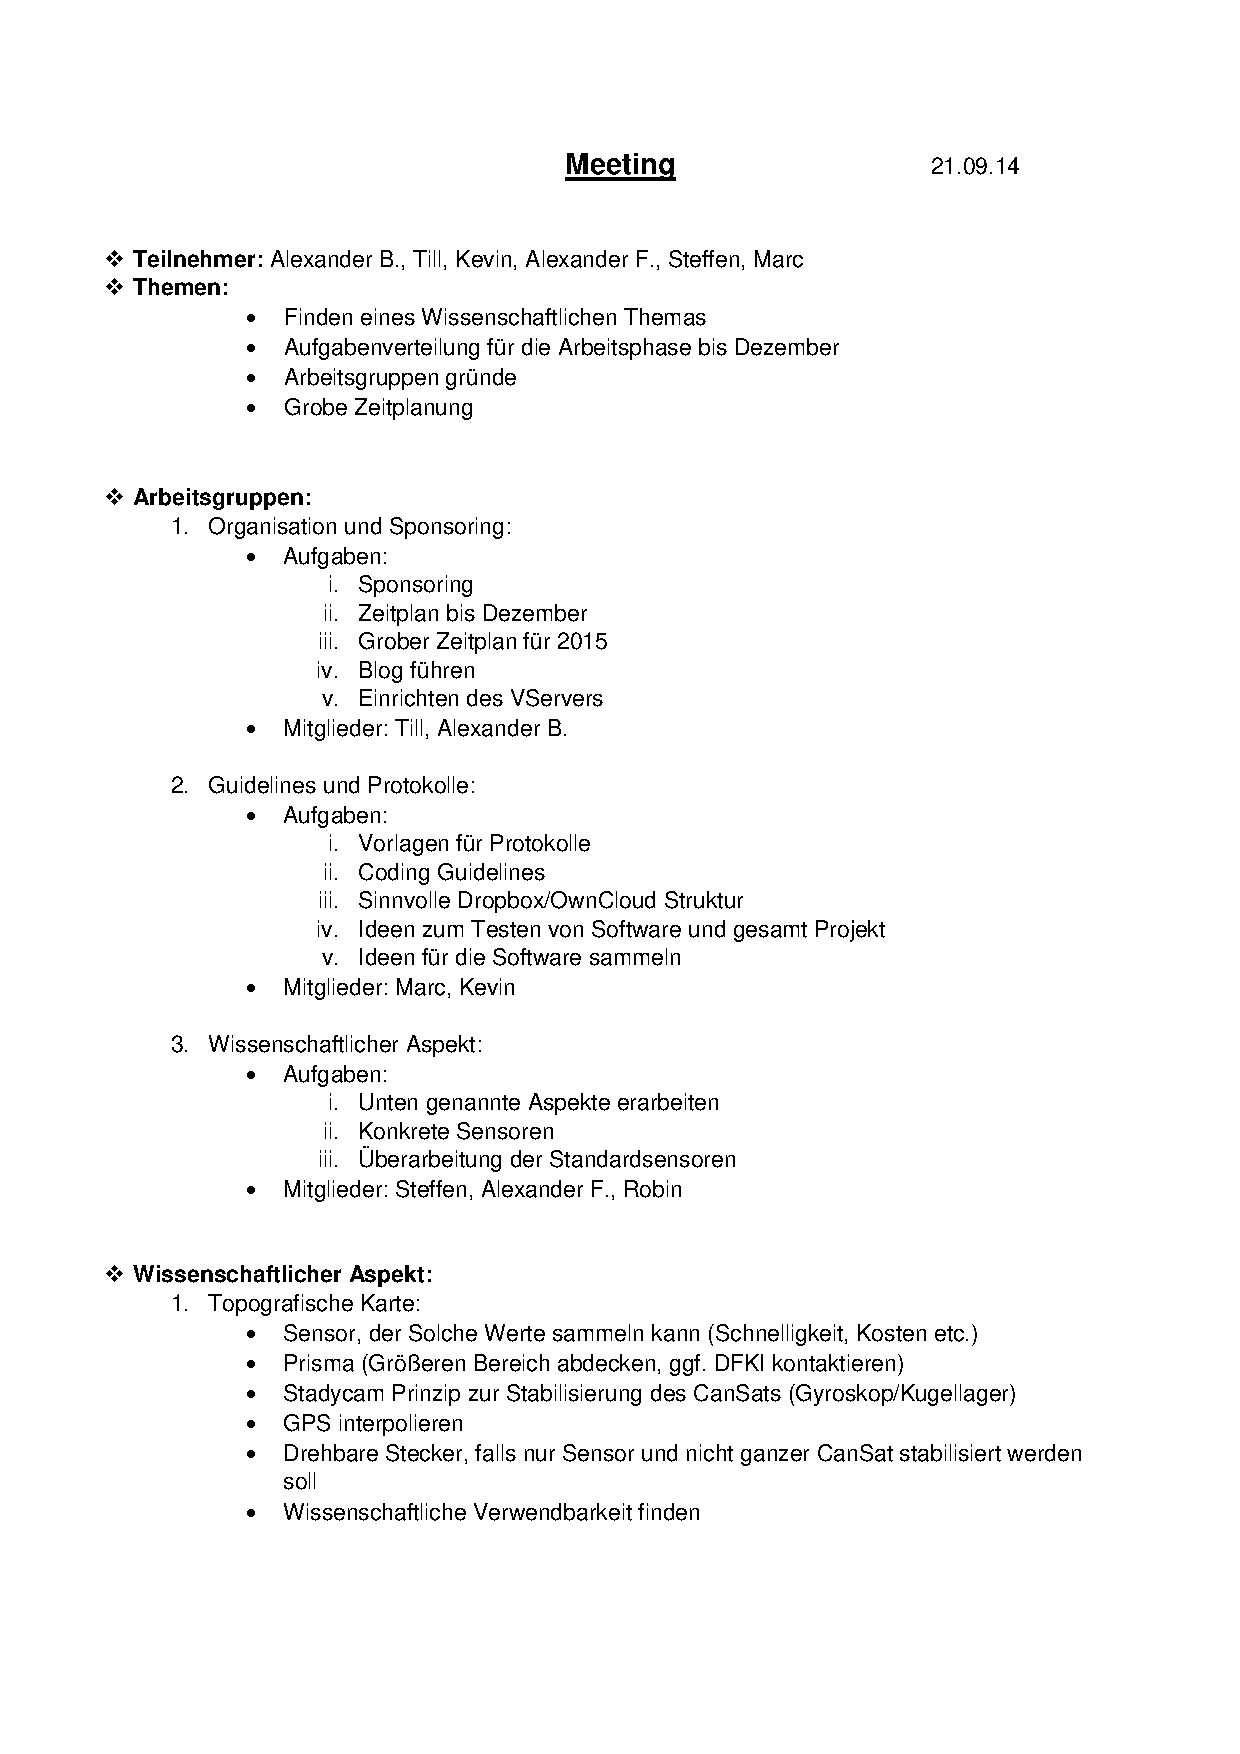
\includepdf[pages=-]{8_Anhang/Protokolle/140921_Meeting_Protokoll}%

\newpage
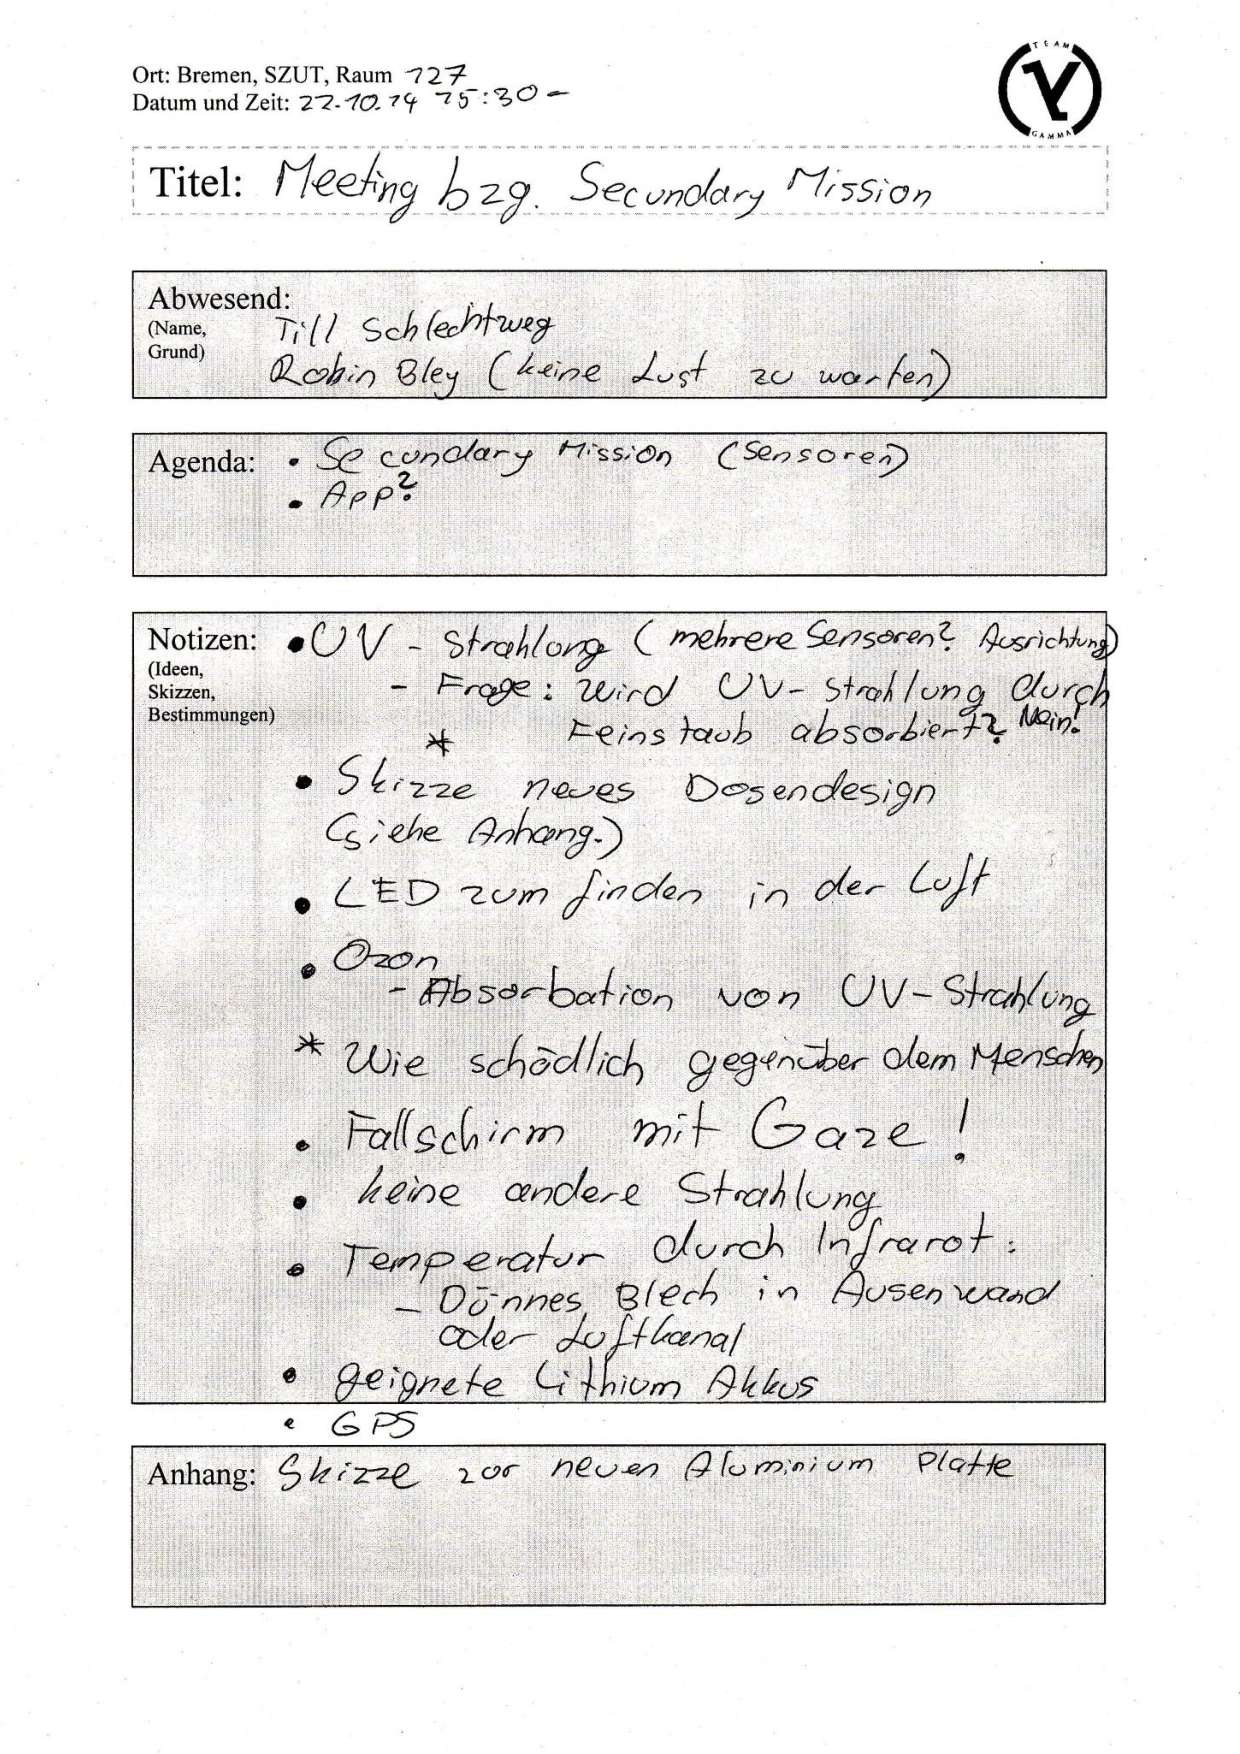
\includepdf[pages=-]{8_Anhang/Protokolle/141022_Meeting_Protokoll}%

\newpage
\begin{figure}[H]
	\centering
	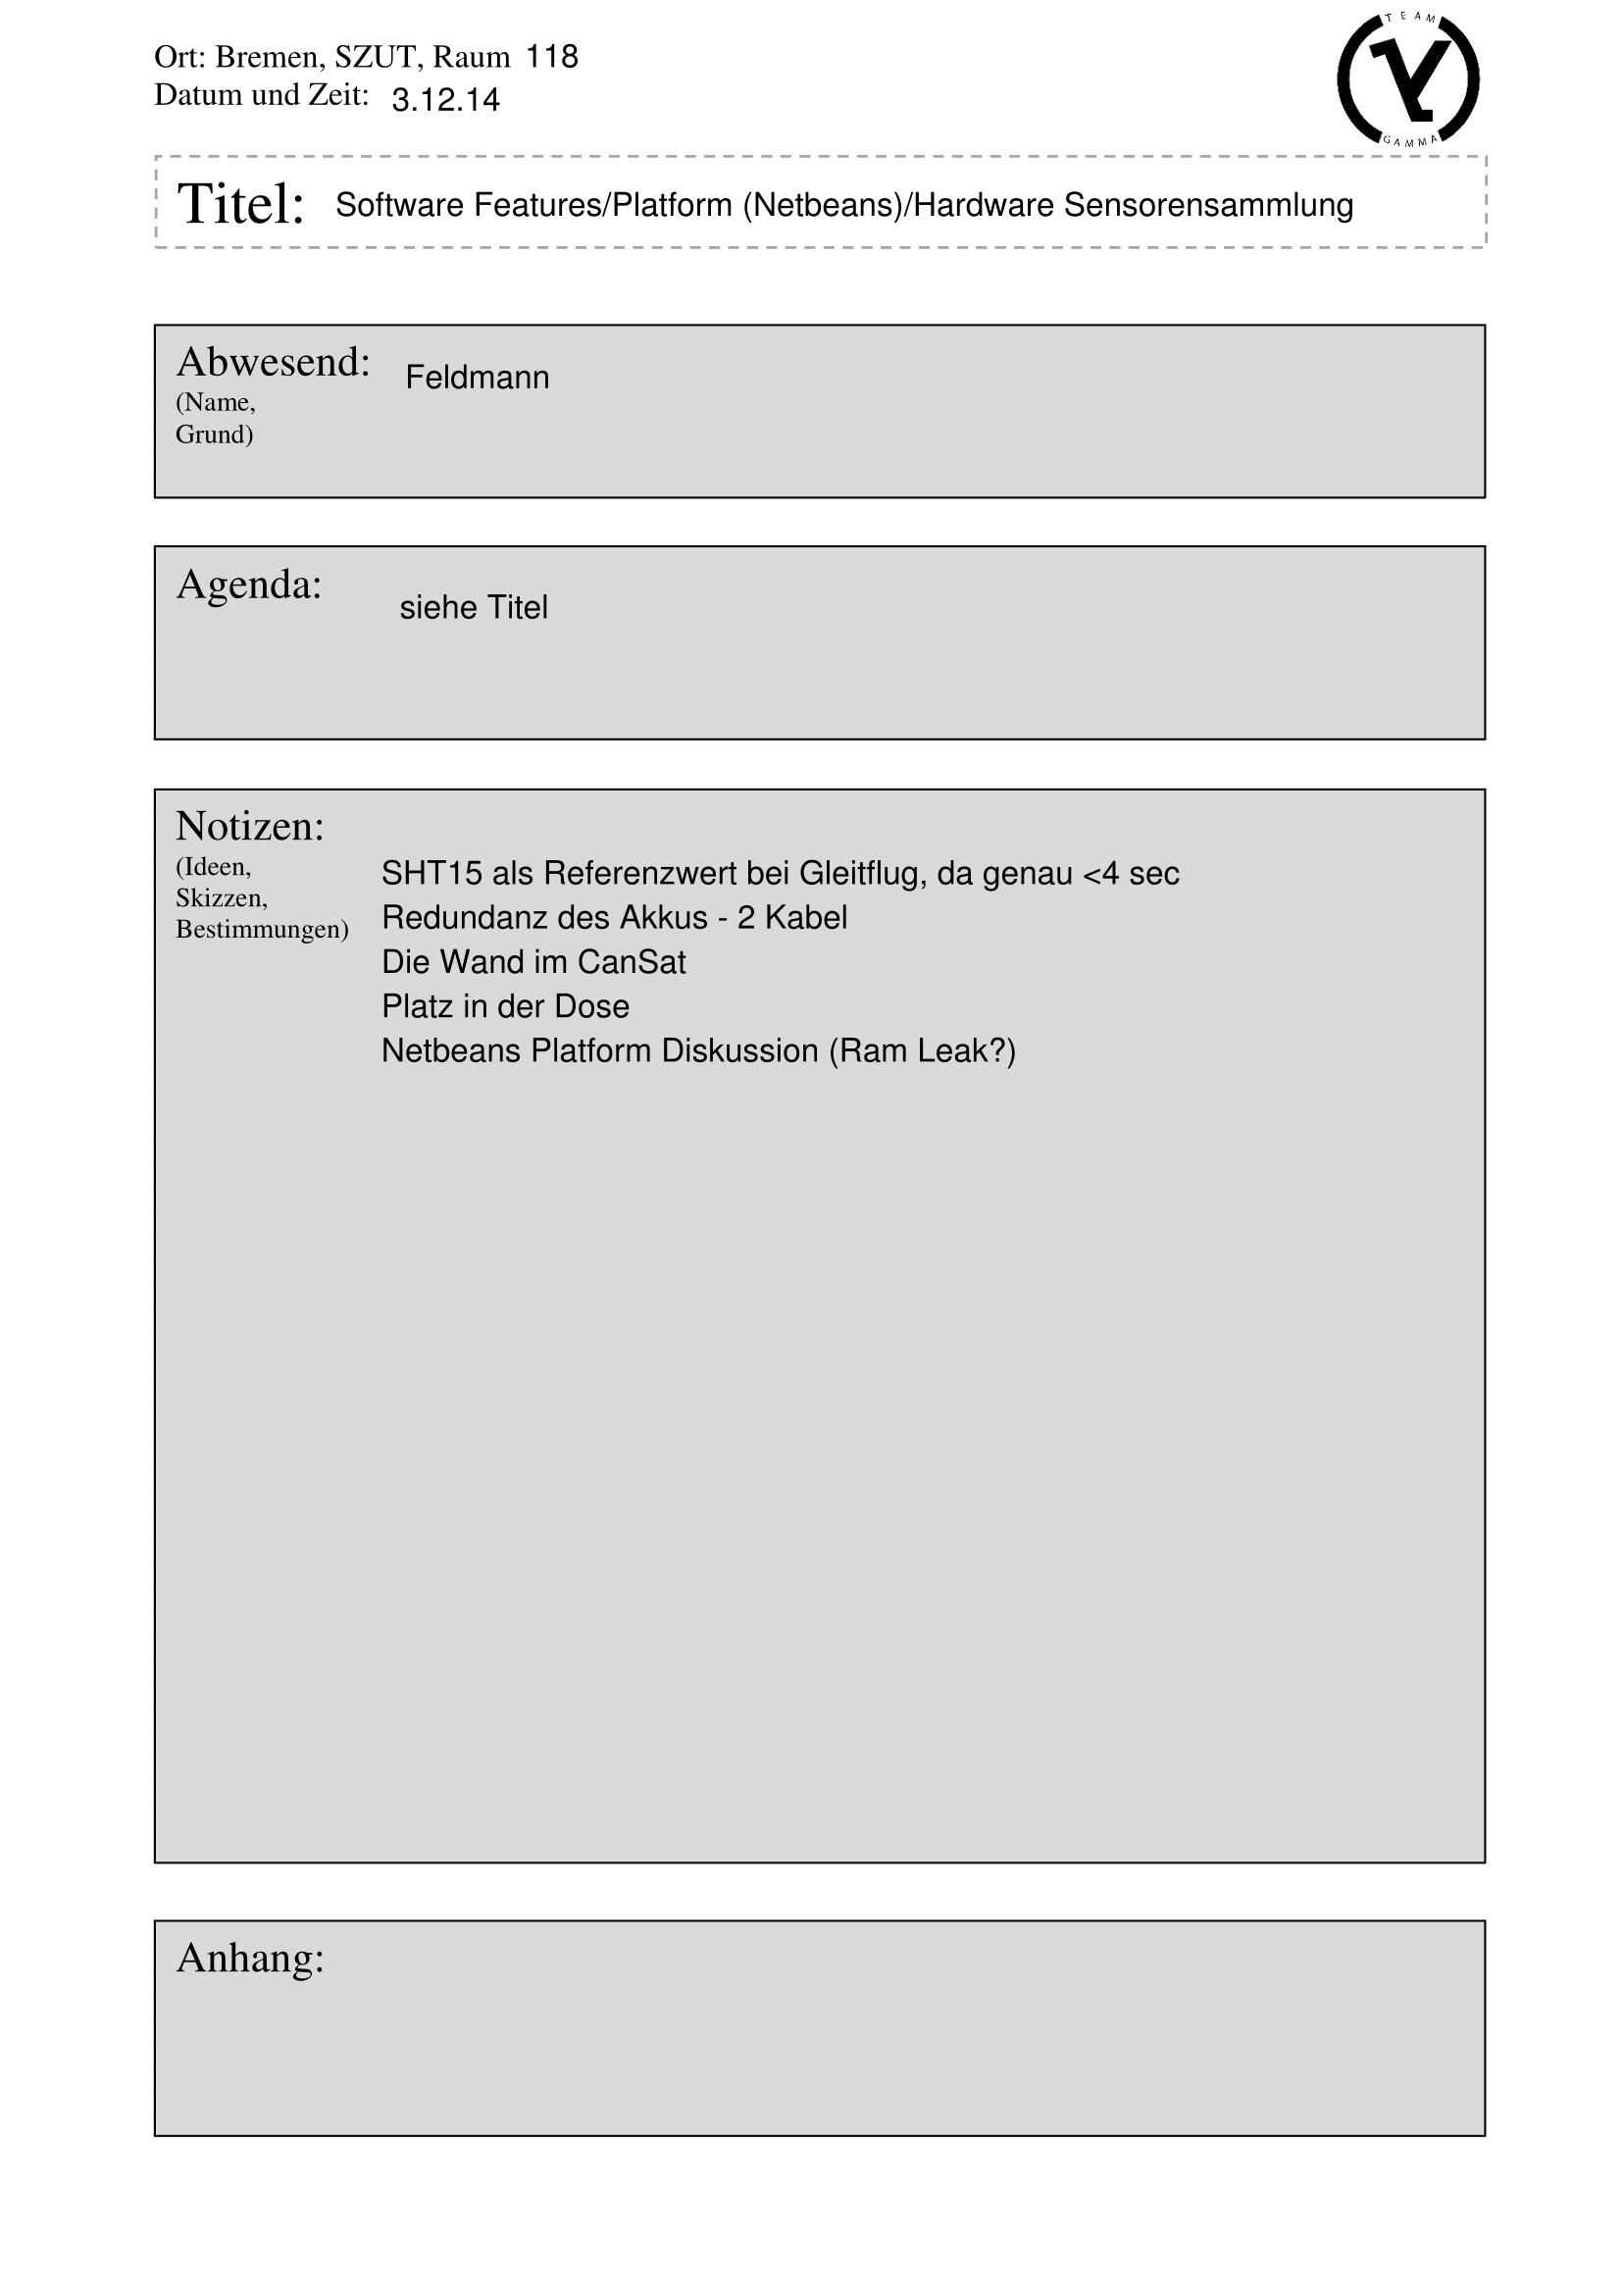
\includegraphics[width=0.8\textwidth]{8_Anhang/Protokolle/141203_Meeting_Protokoll.png}%
	\label{pic_protokoll_140203}
\end{figure}

\newpage
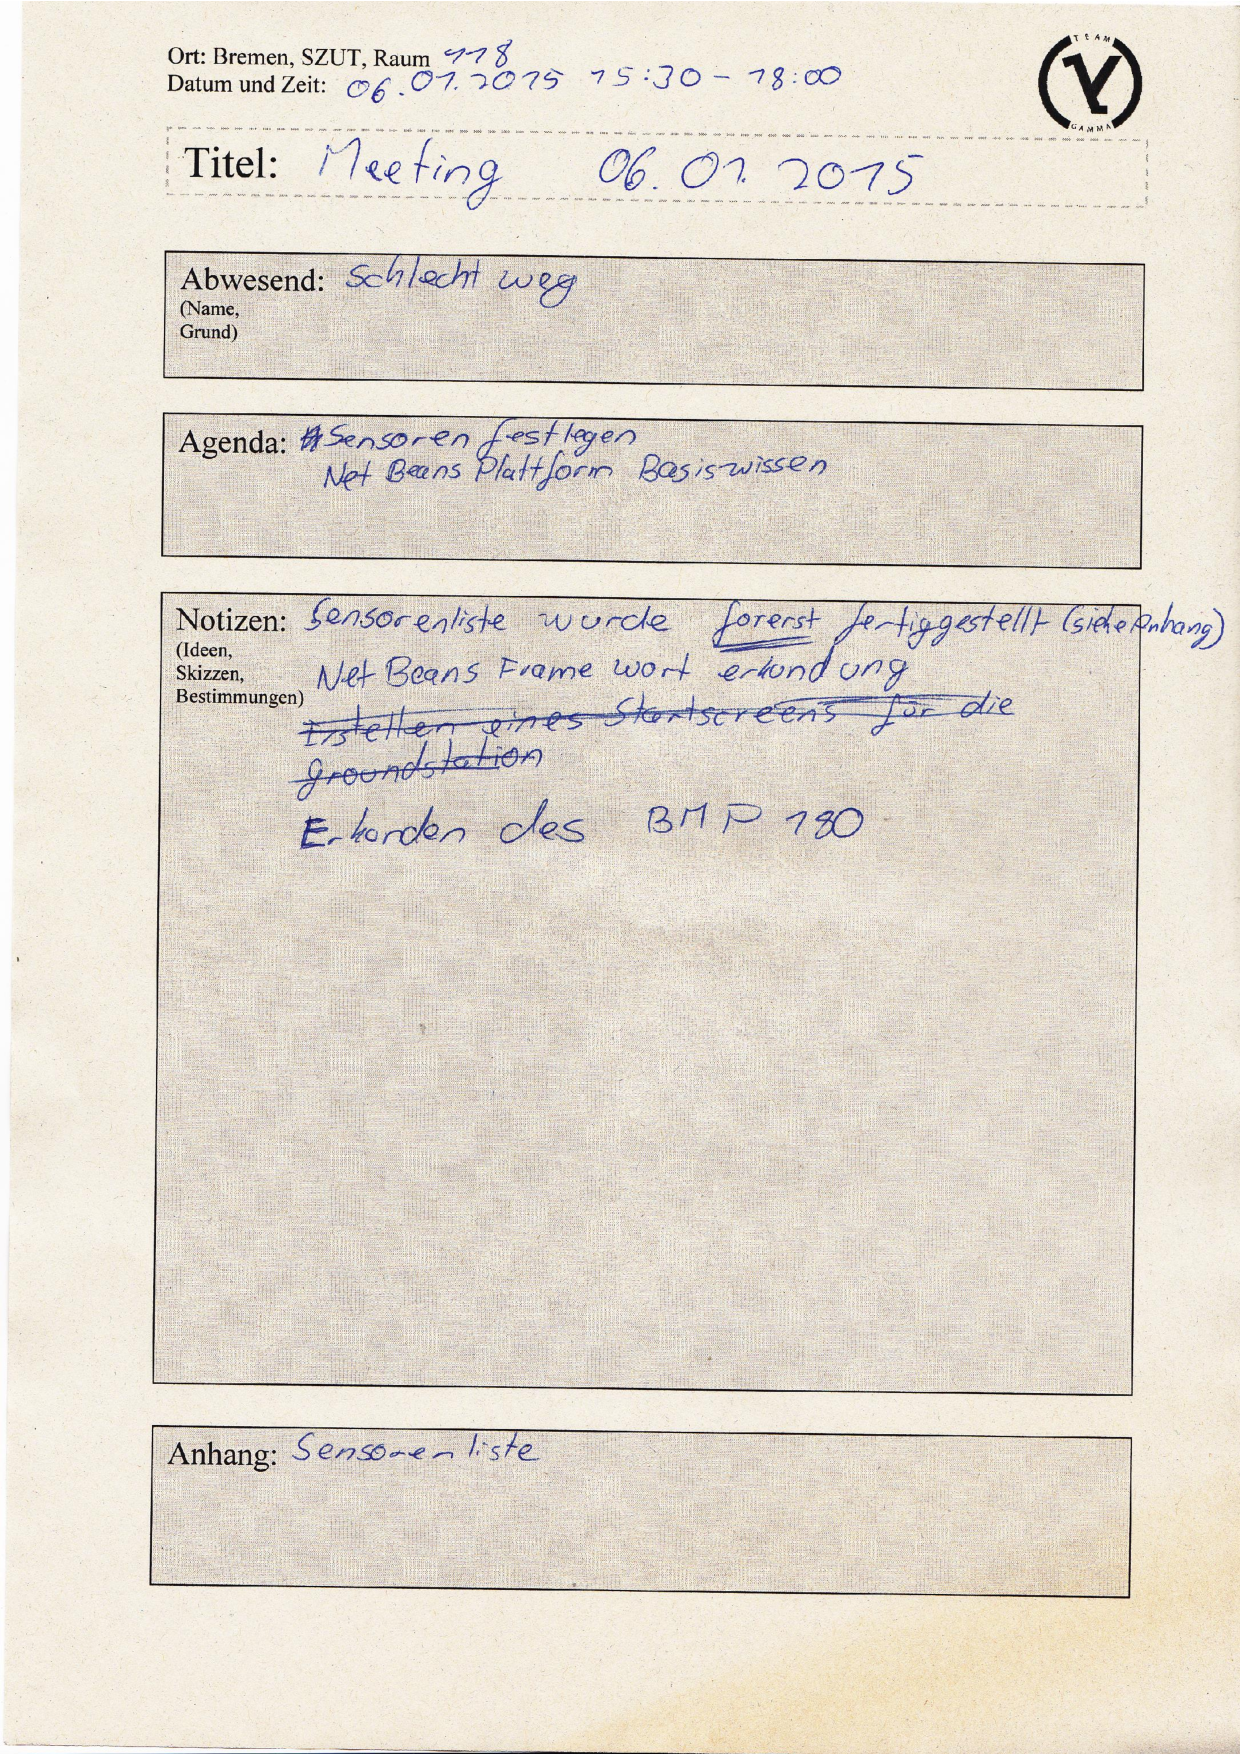
\includepdf{8_Anhang/Protokolle/150106_Meeting_Protokoll}%
\newpage

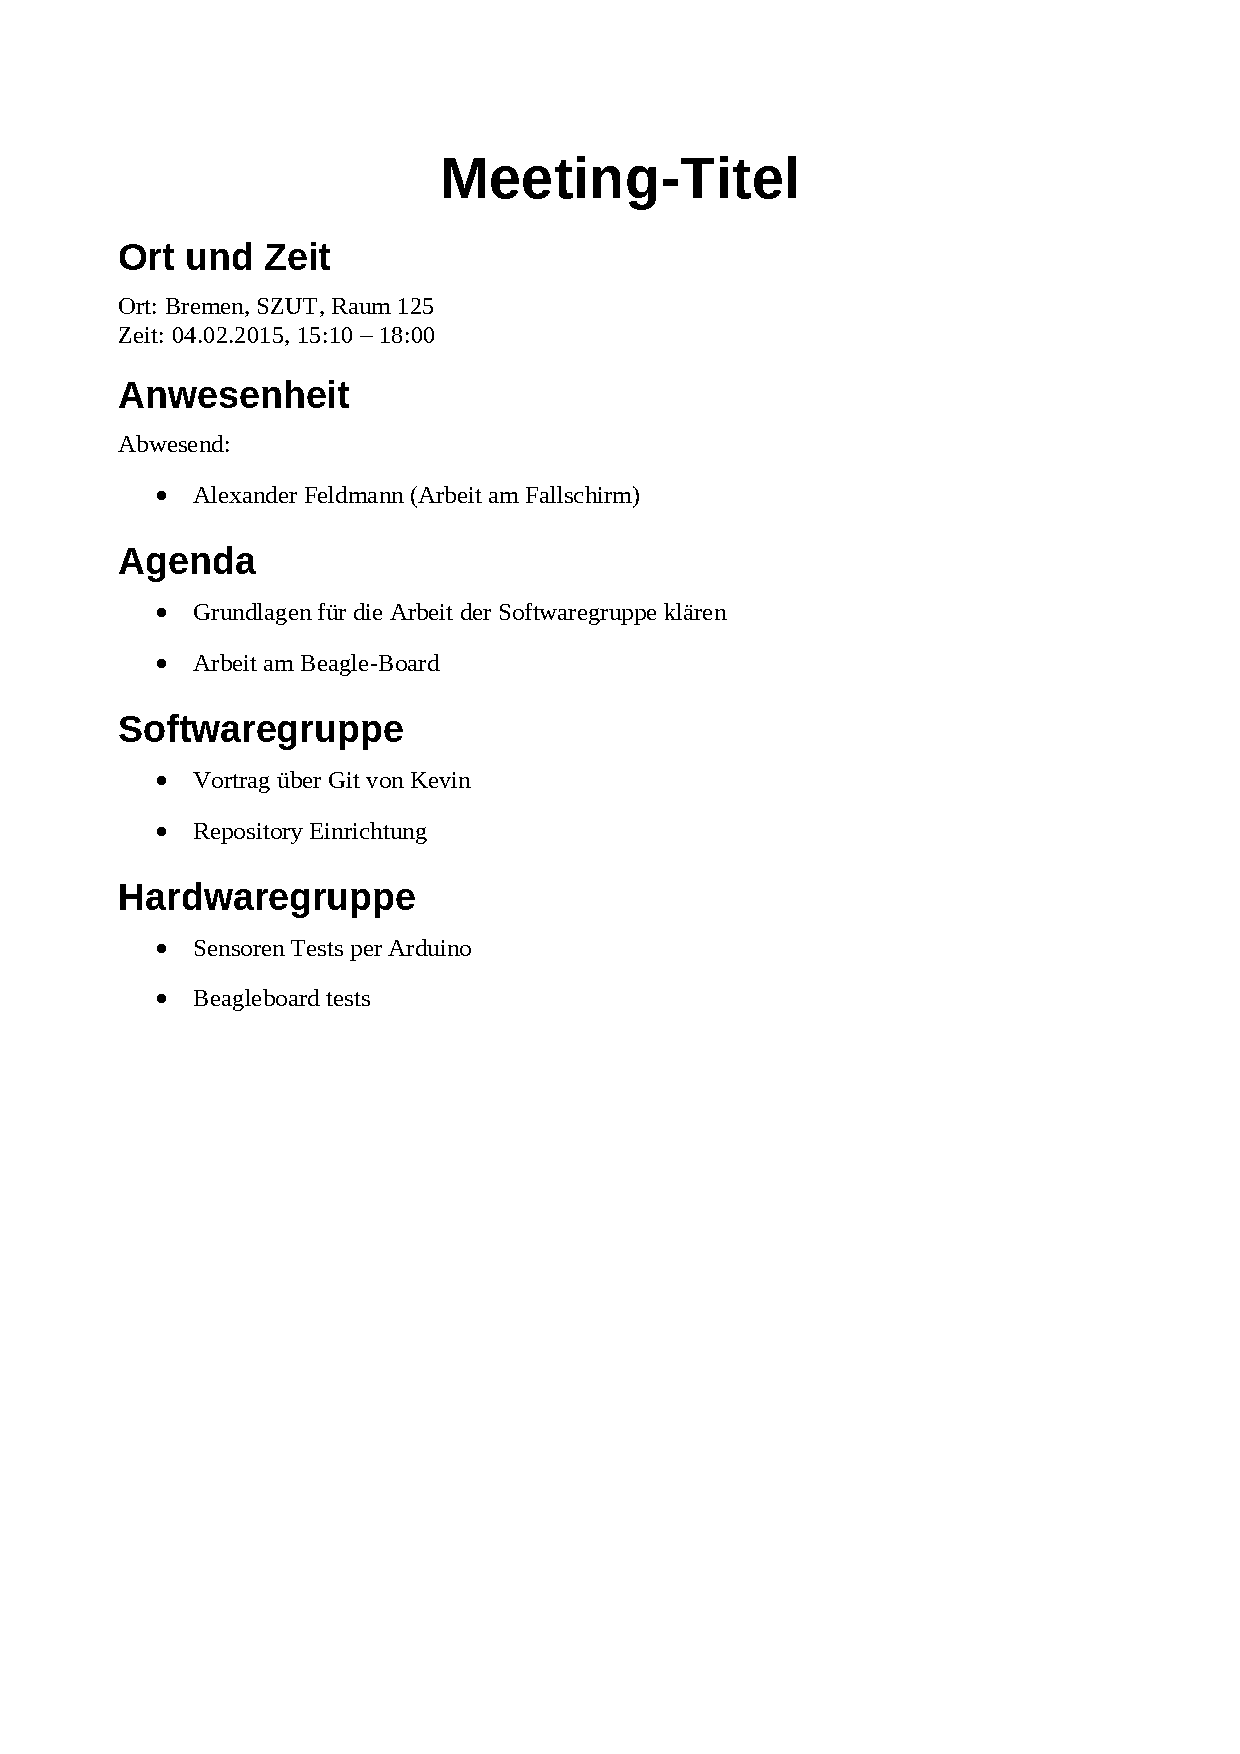
\includepdf{8_Anhang/Protokolle/150204_Meeting_Protokoll}%
\newpage
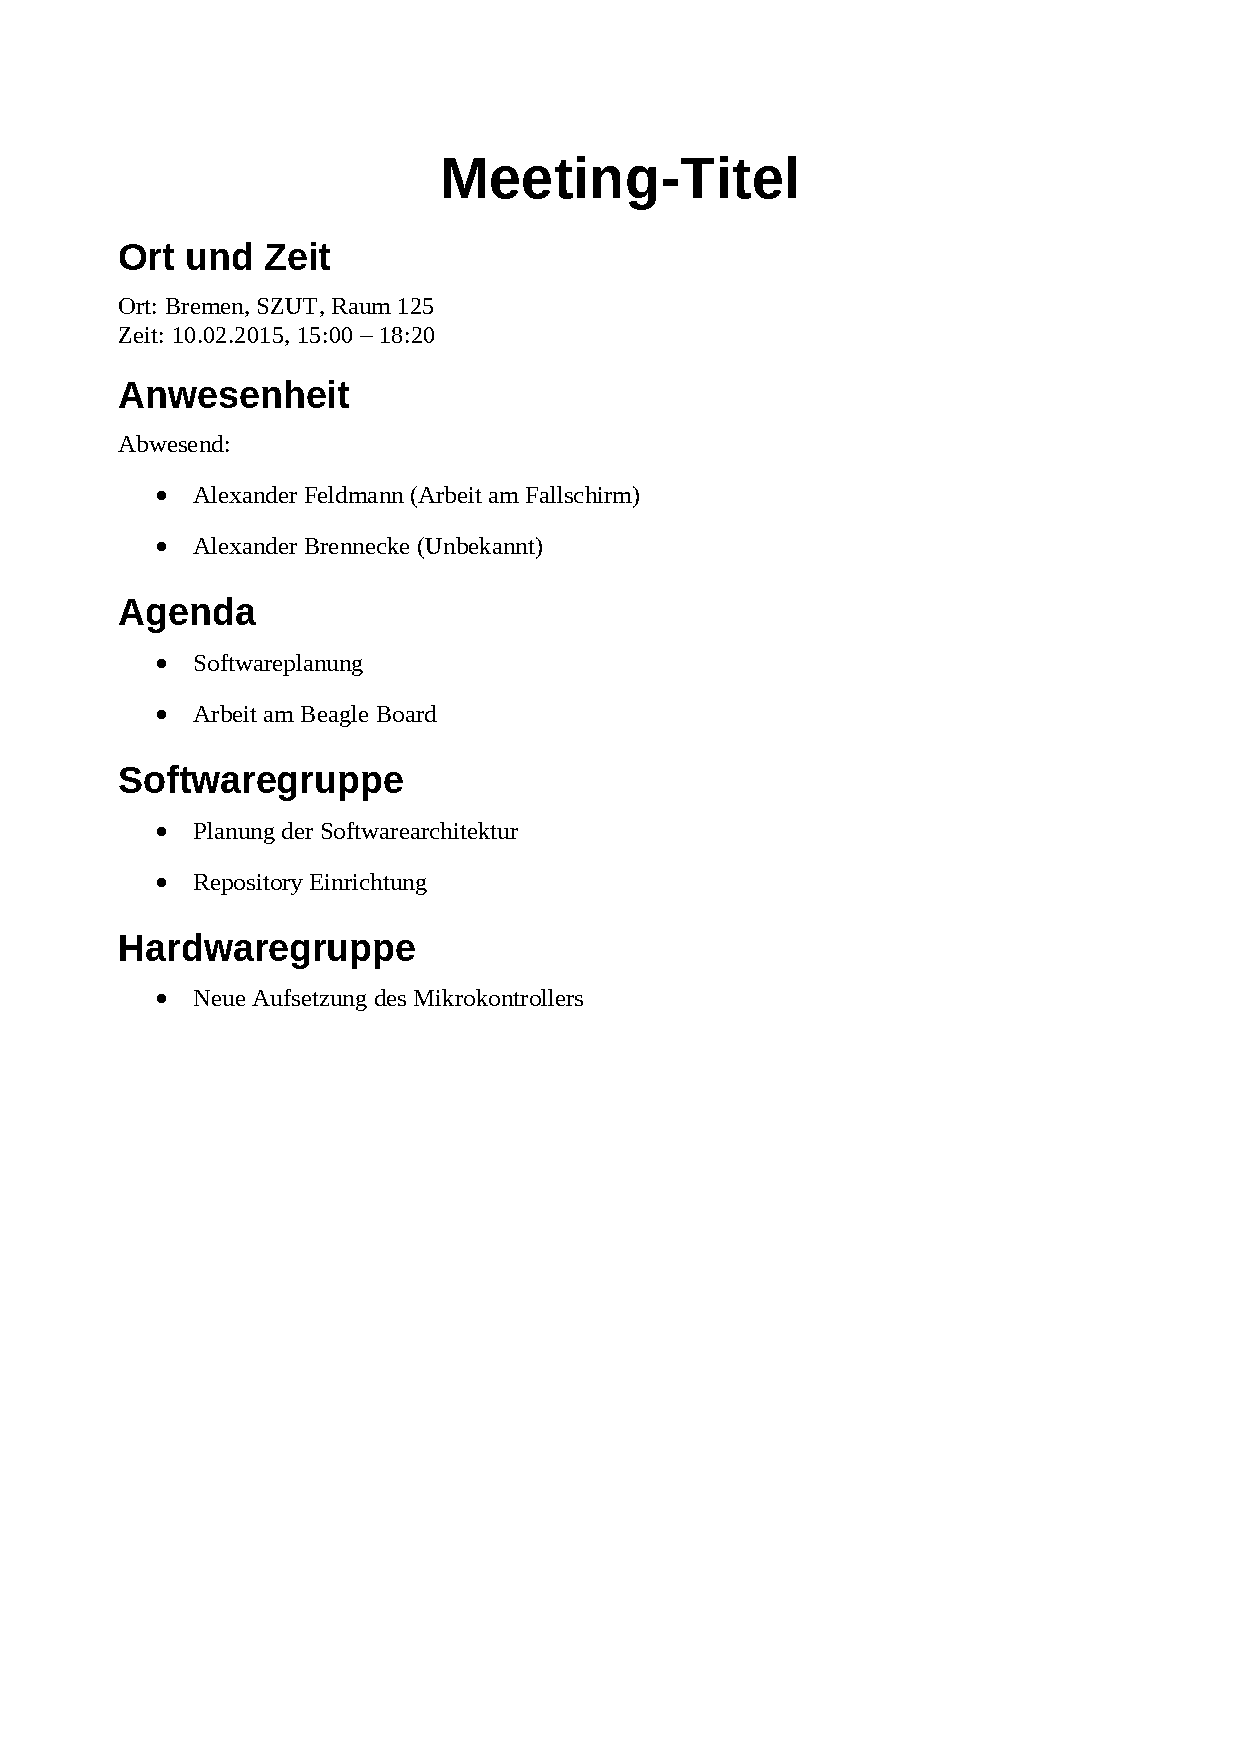
\includepdf{8_Anhang/Protokolle/150210_Meeting_Protokoll}%
\newpage
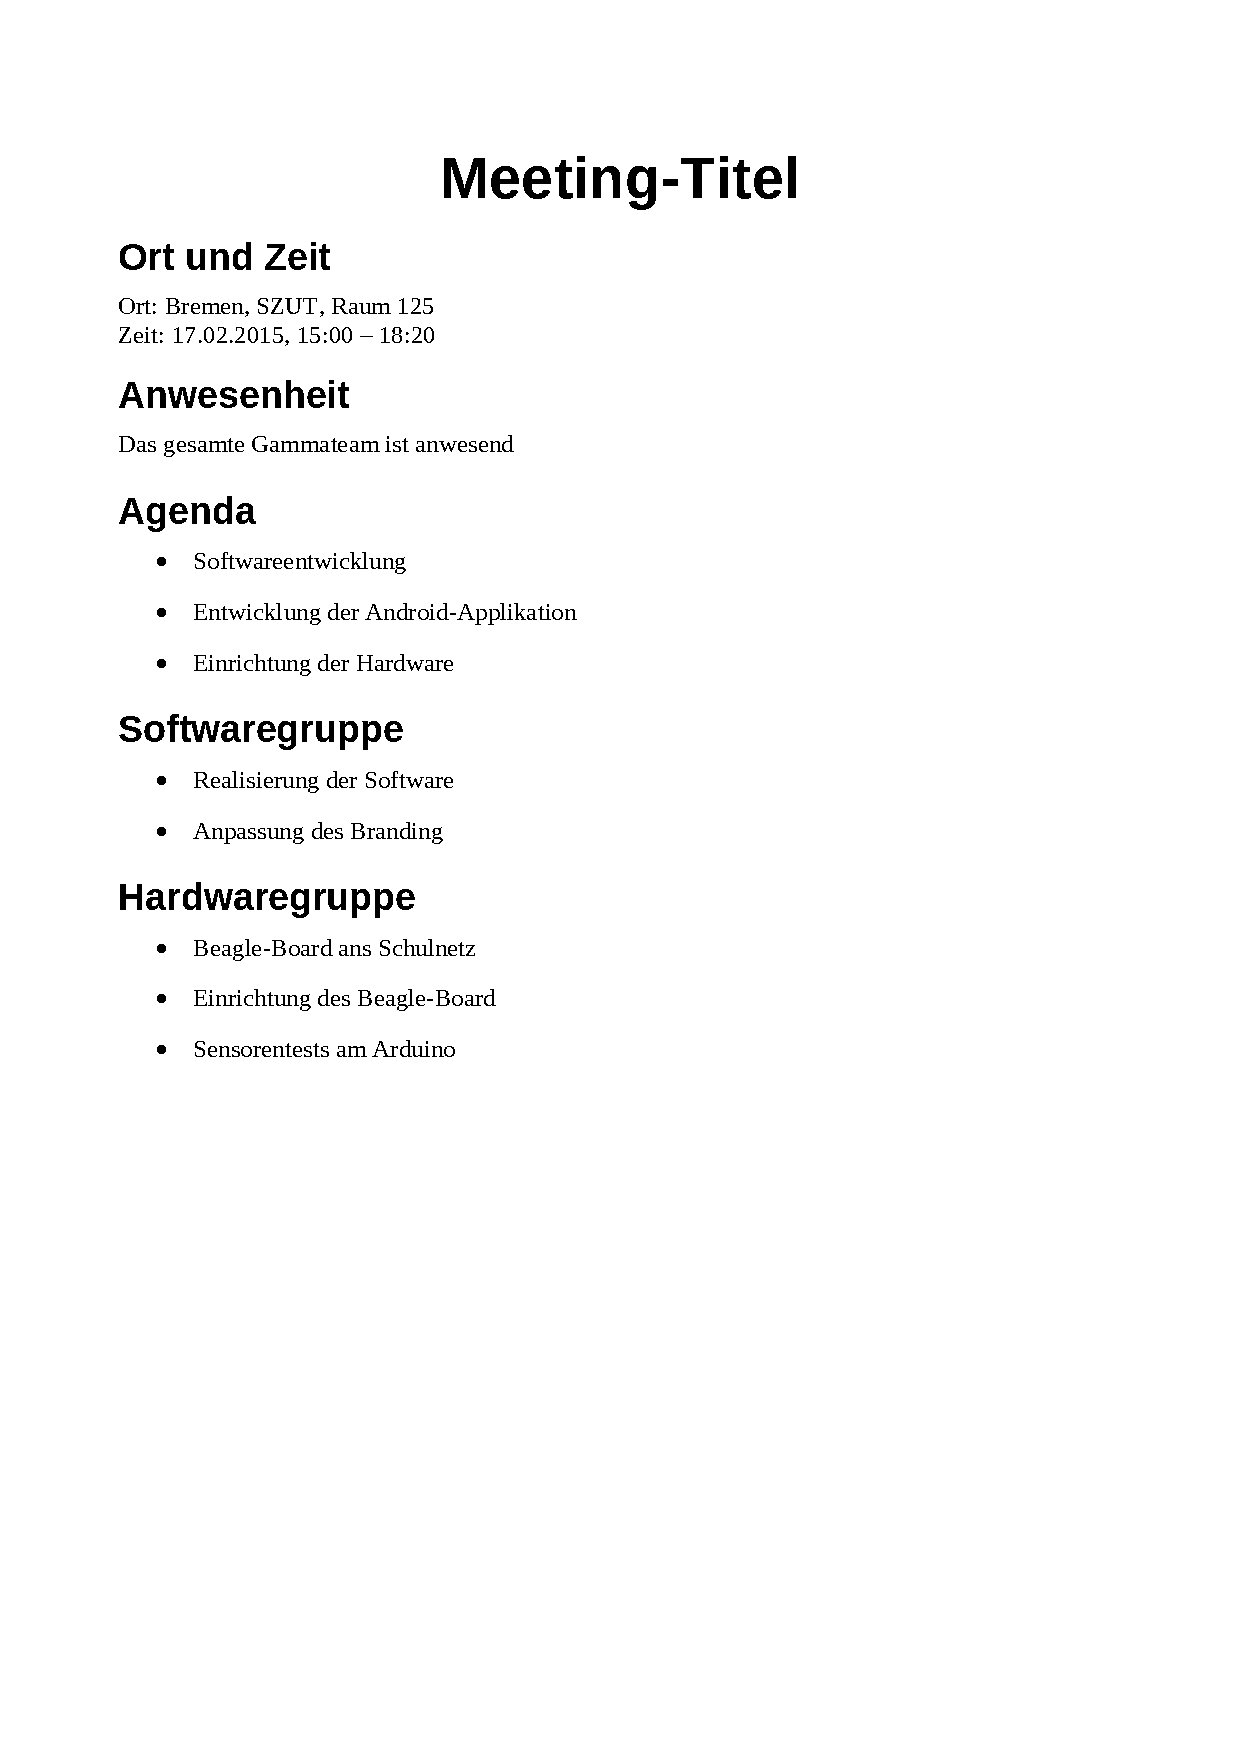
\includepdf{8_Anhang/Protokolle/150217_Meeting_Protokoll}%
\newpage
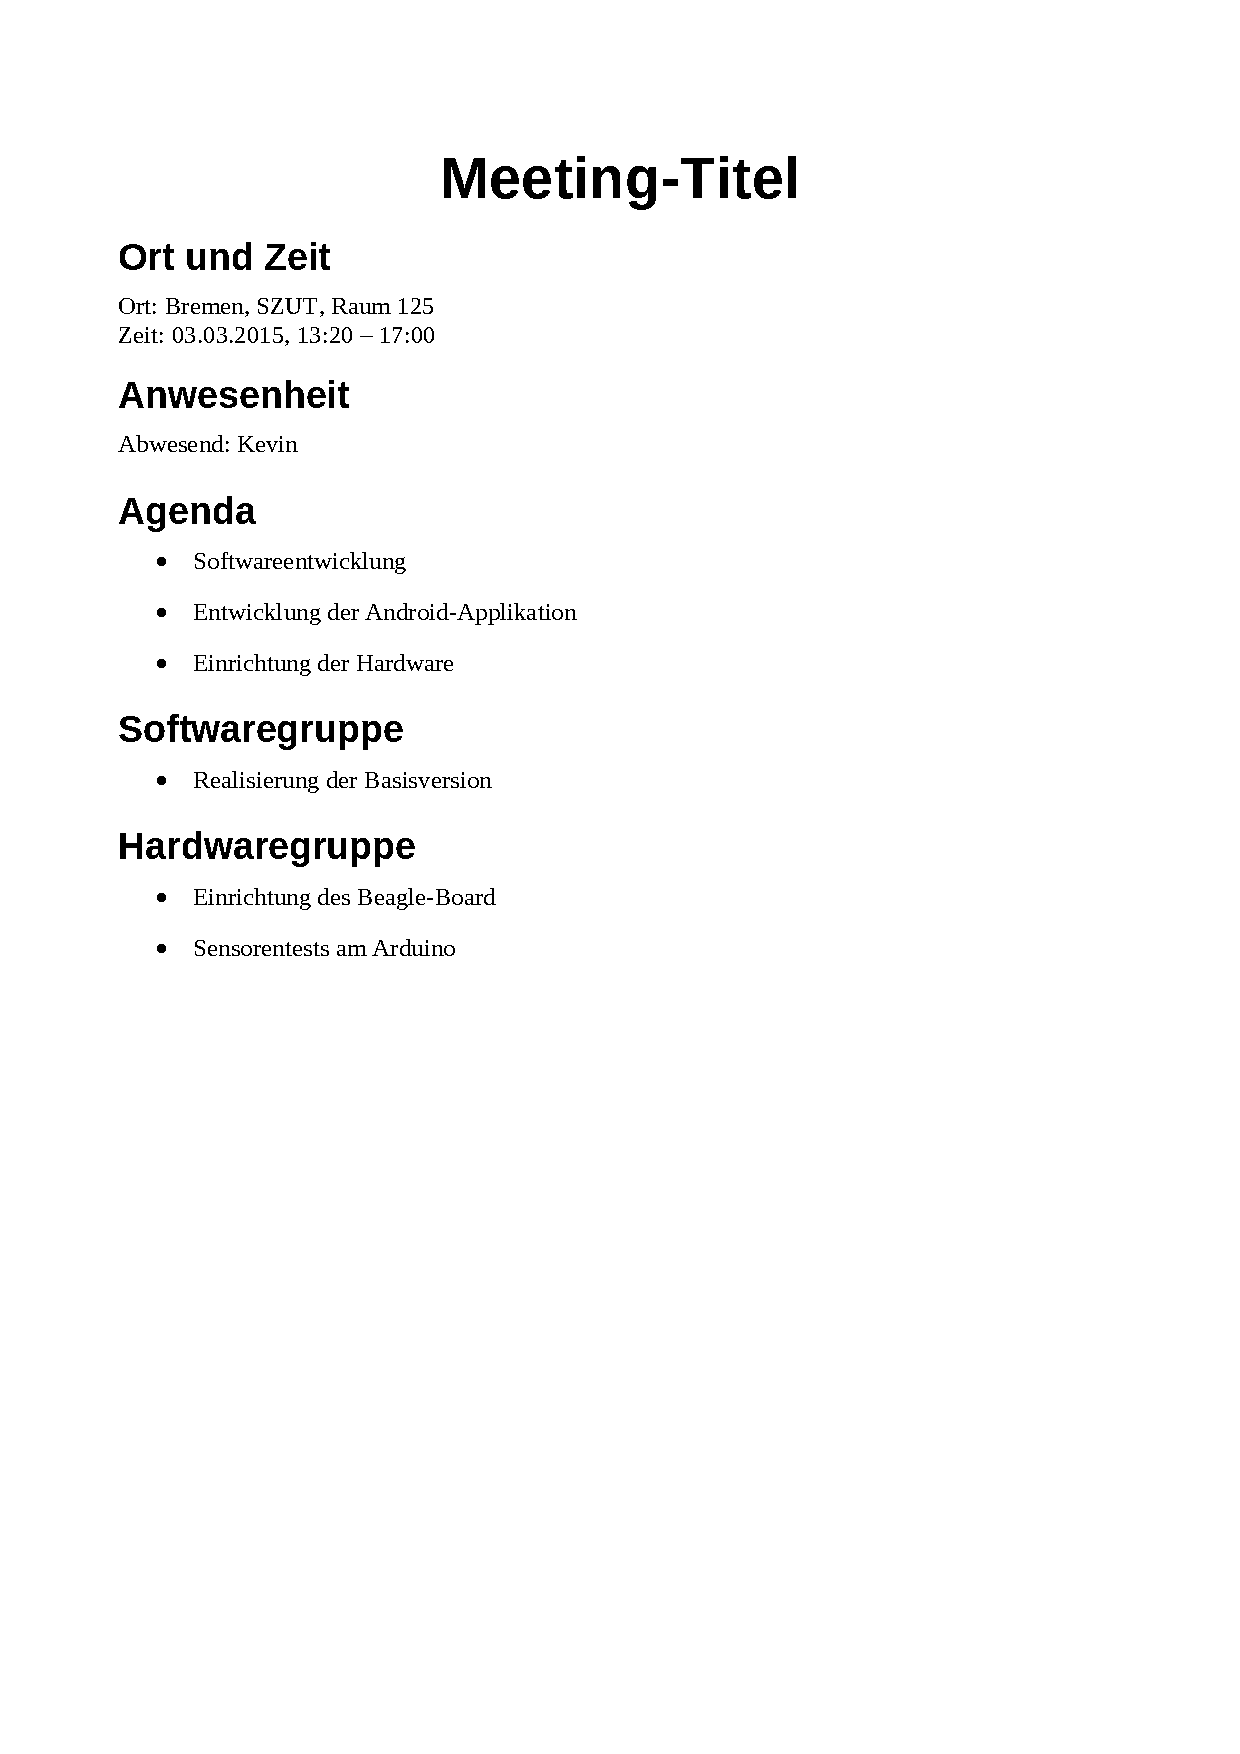
\includepdf{8_Anhang/Protokolle/150303_Meeting_Protokoll}%
\newpage
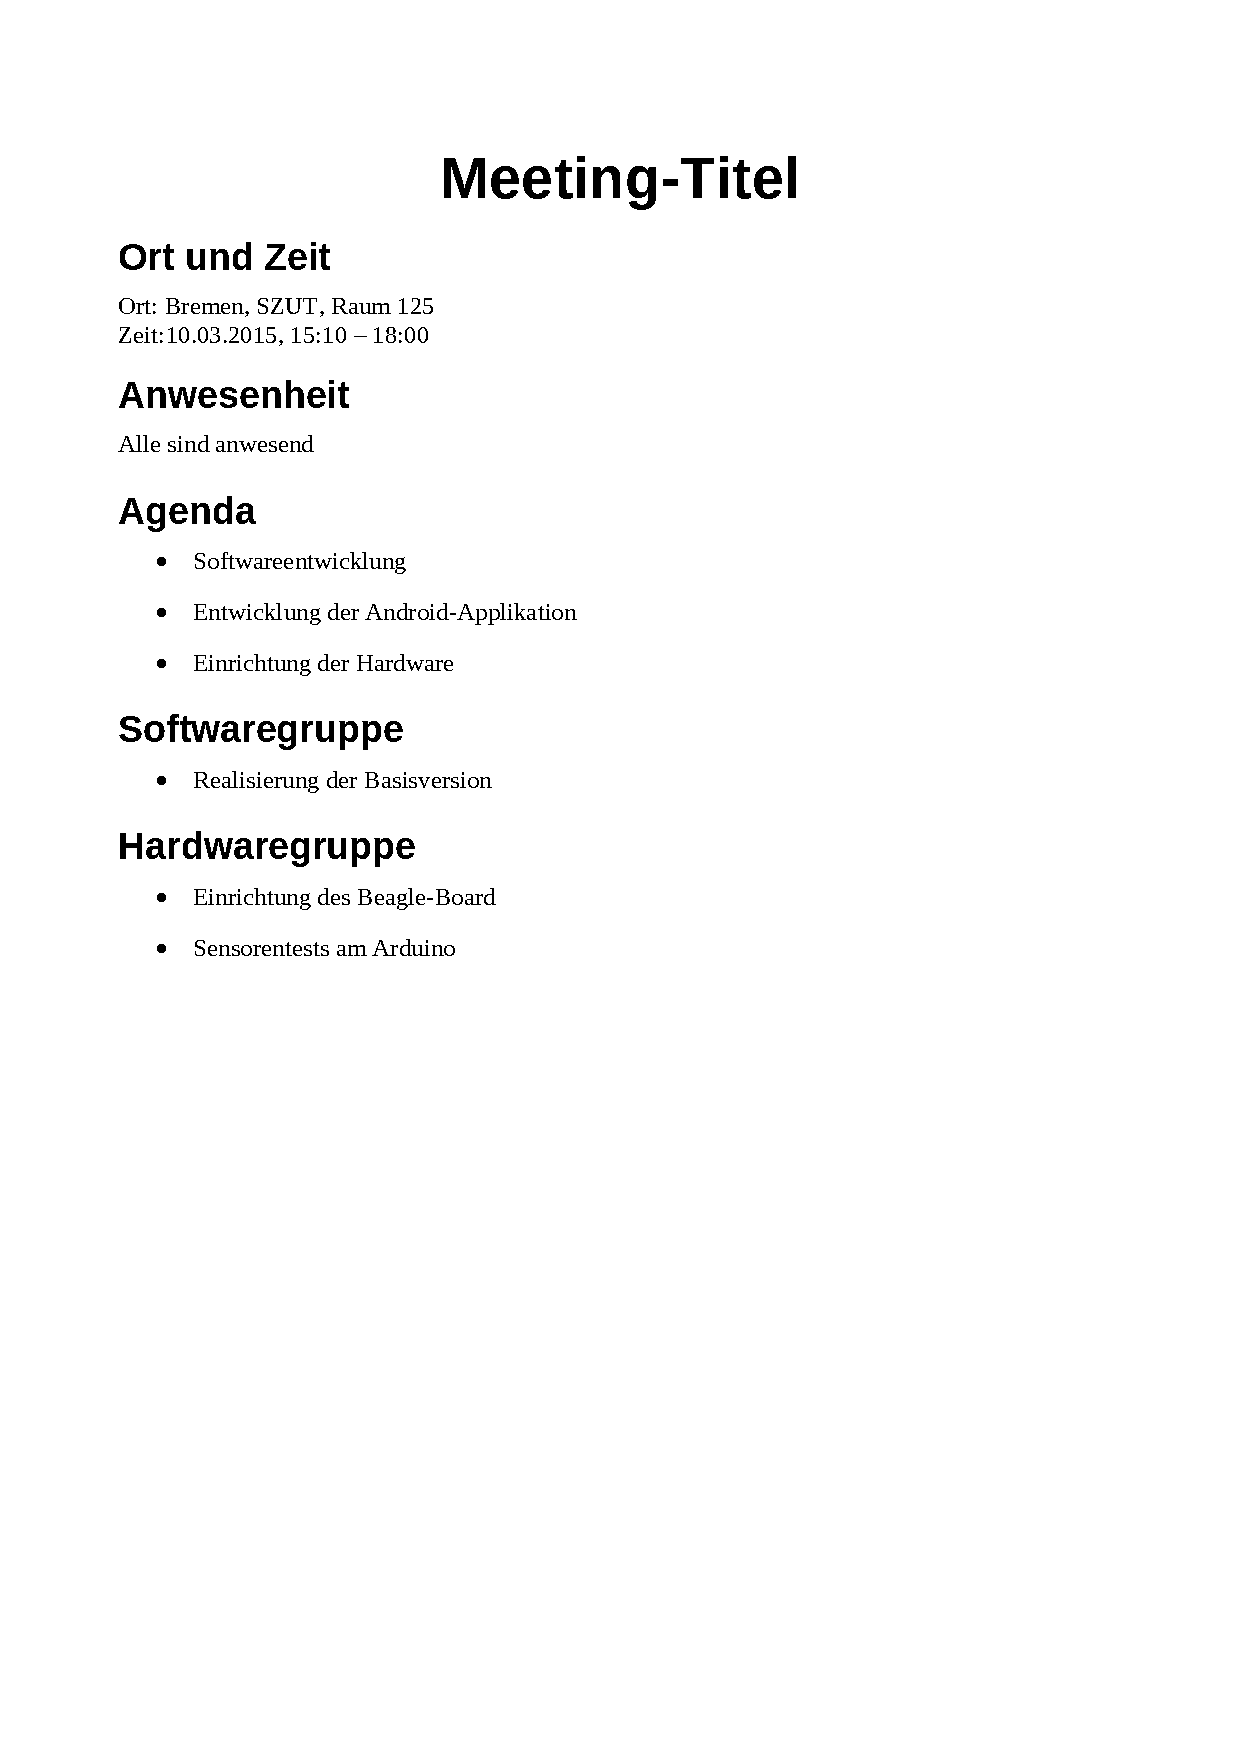
\includepdf{8_Anhang/Protokolle/150310_Meeting_Protokoll}%
\newpage
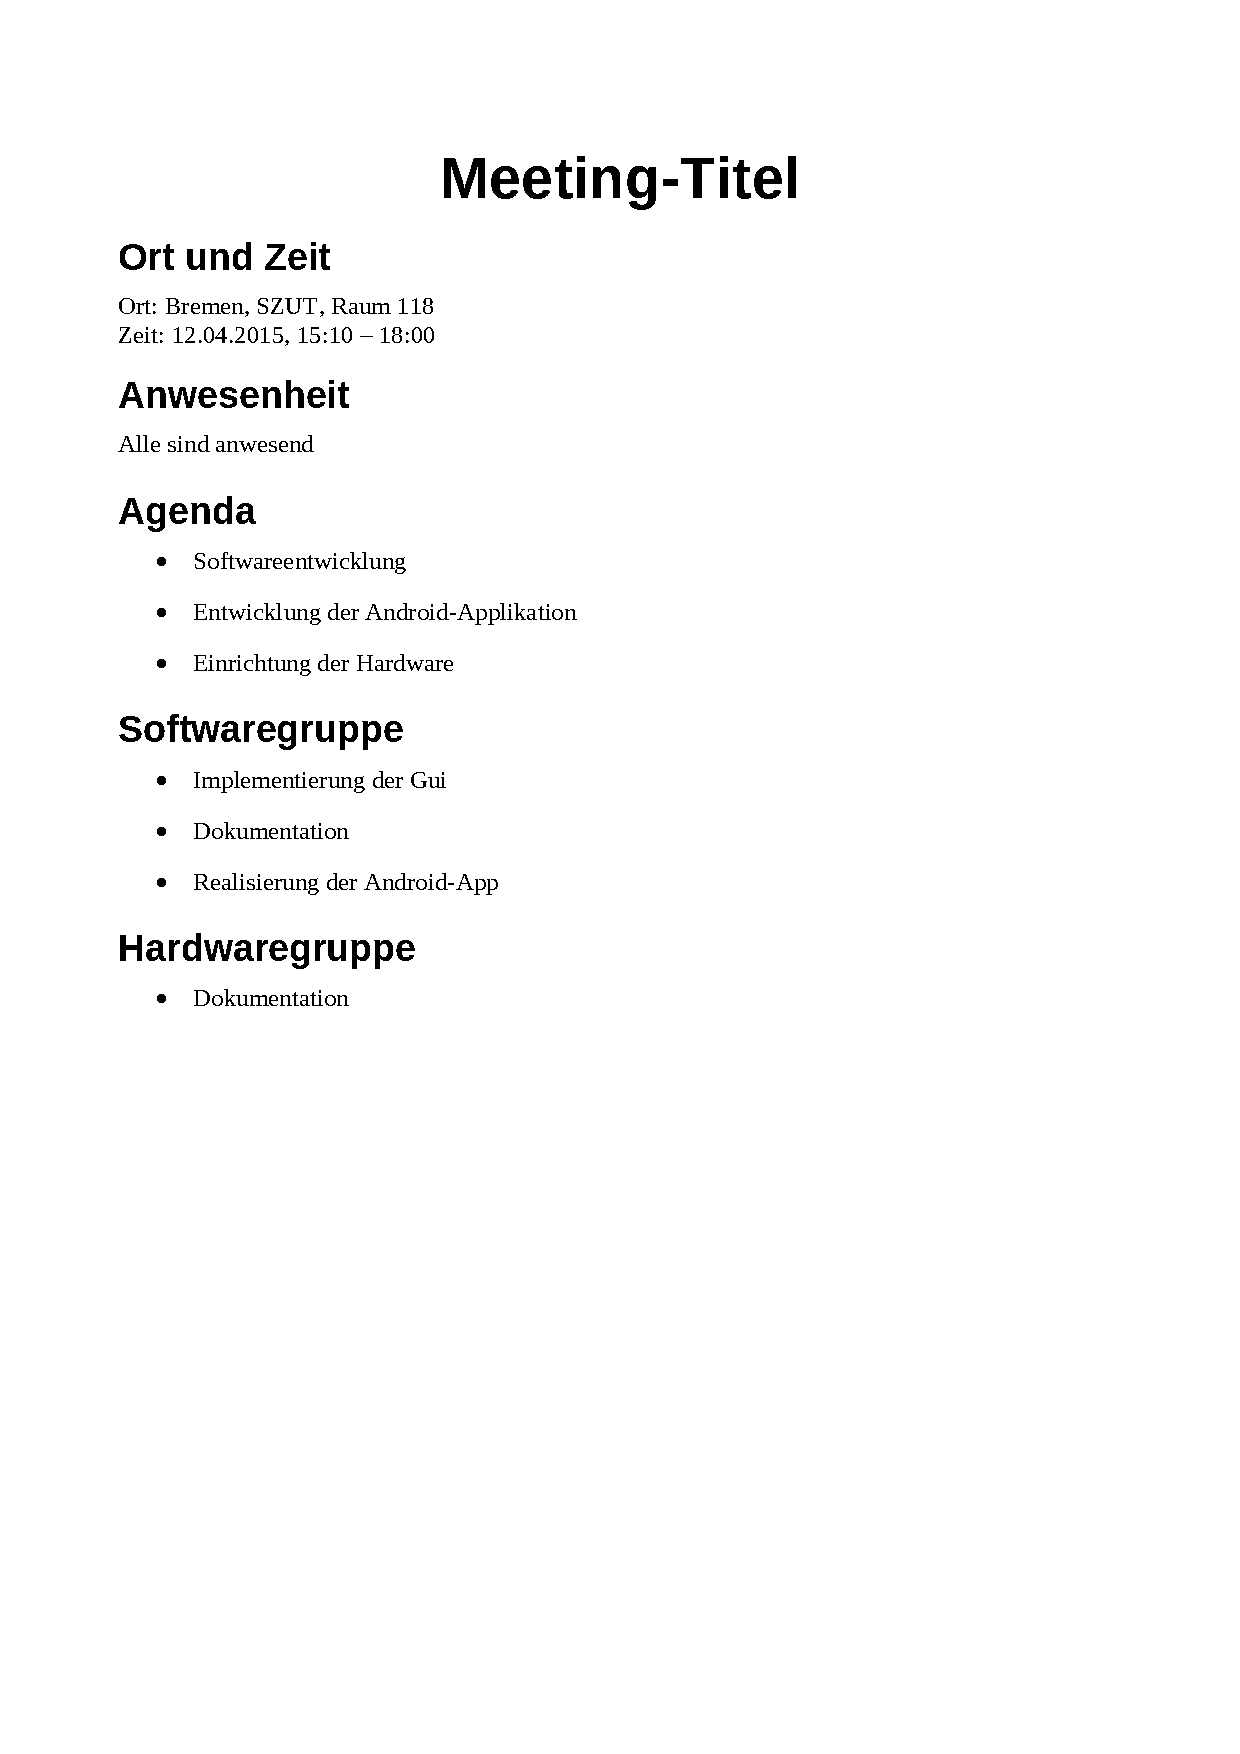
\includepdf{8_Anhang/Protokolle/150317_Meeting_Protokoll}%
\newpage
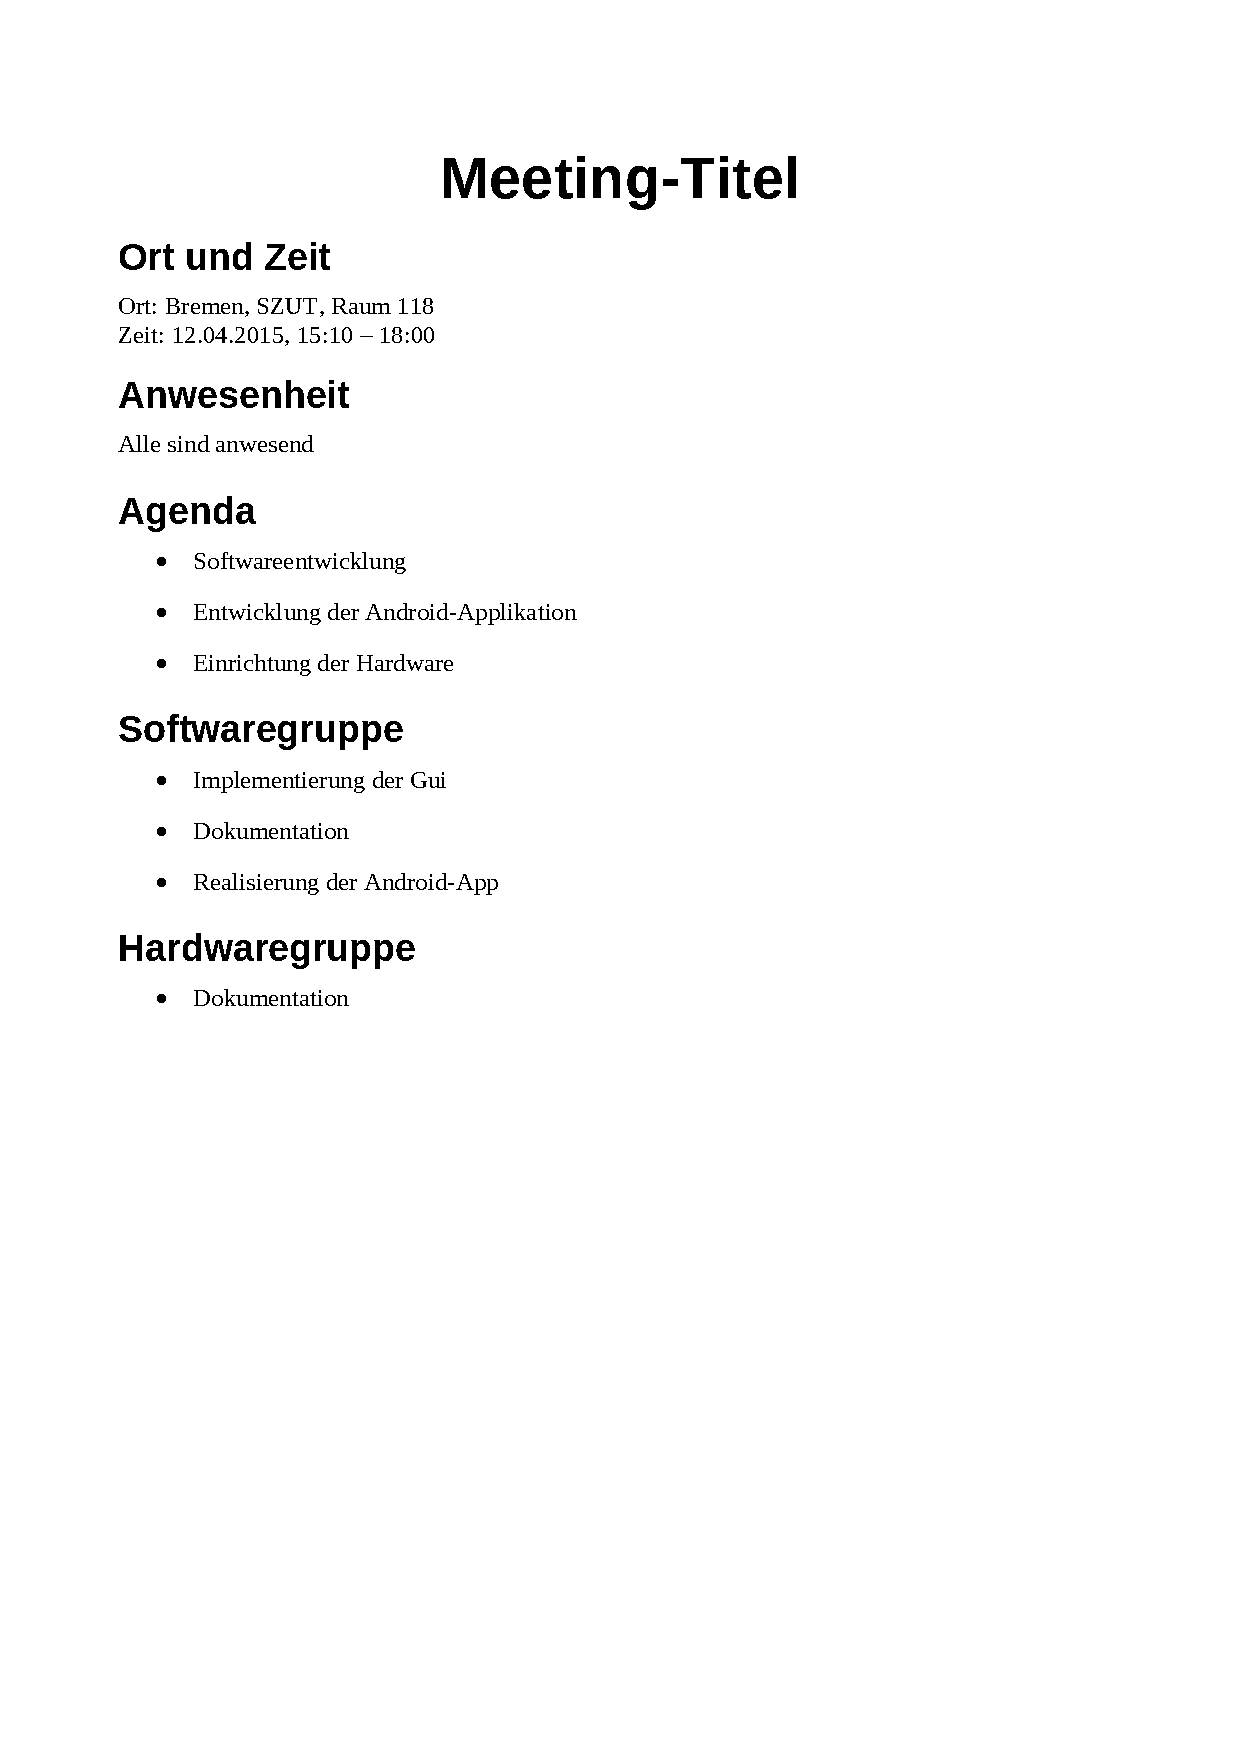
\includepdf{8_Anhang/Protokolle/150412_Meeting_Protokoll}%
\newpage
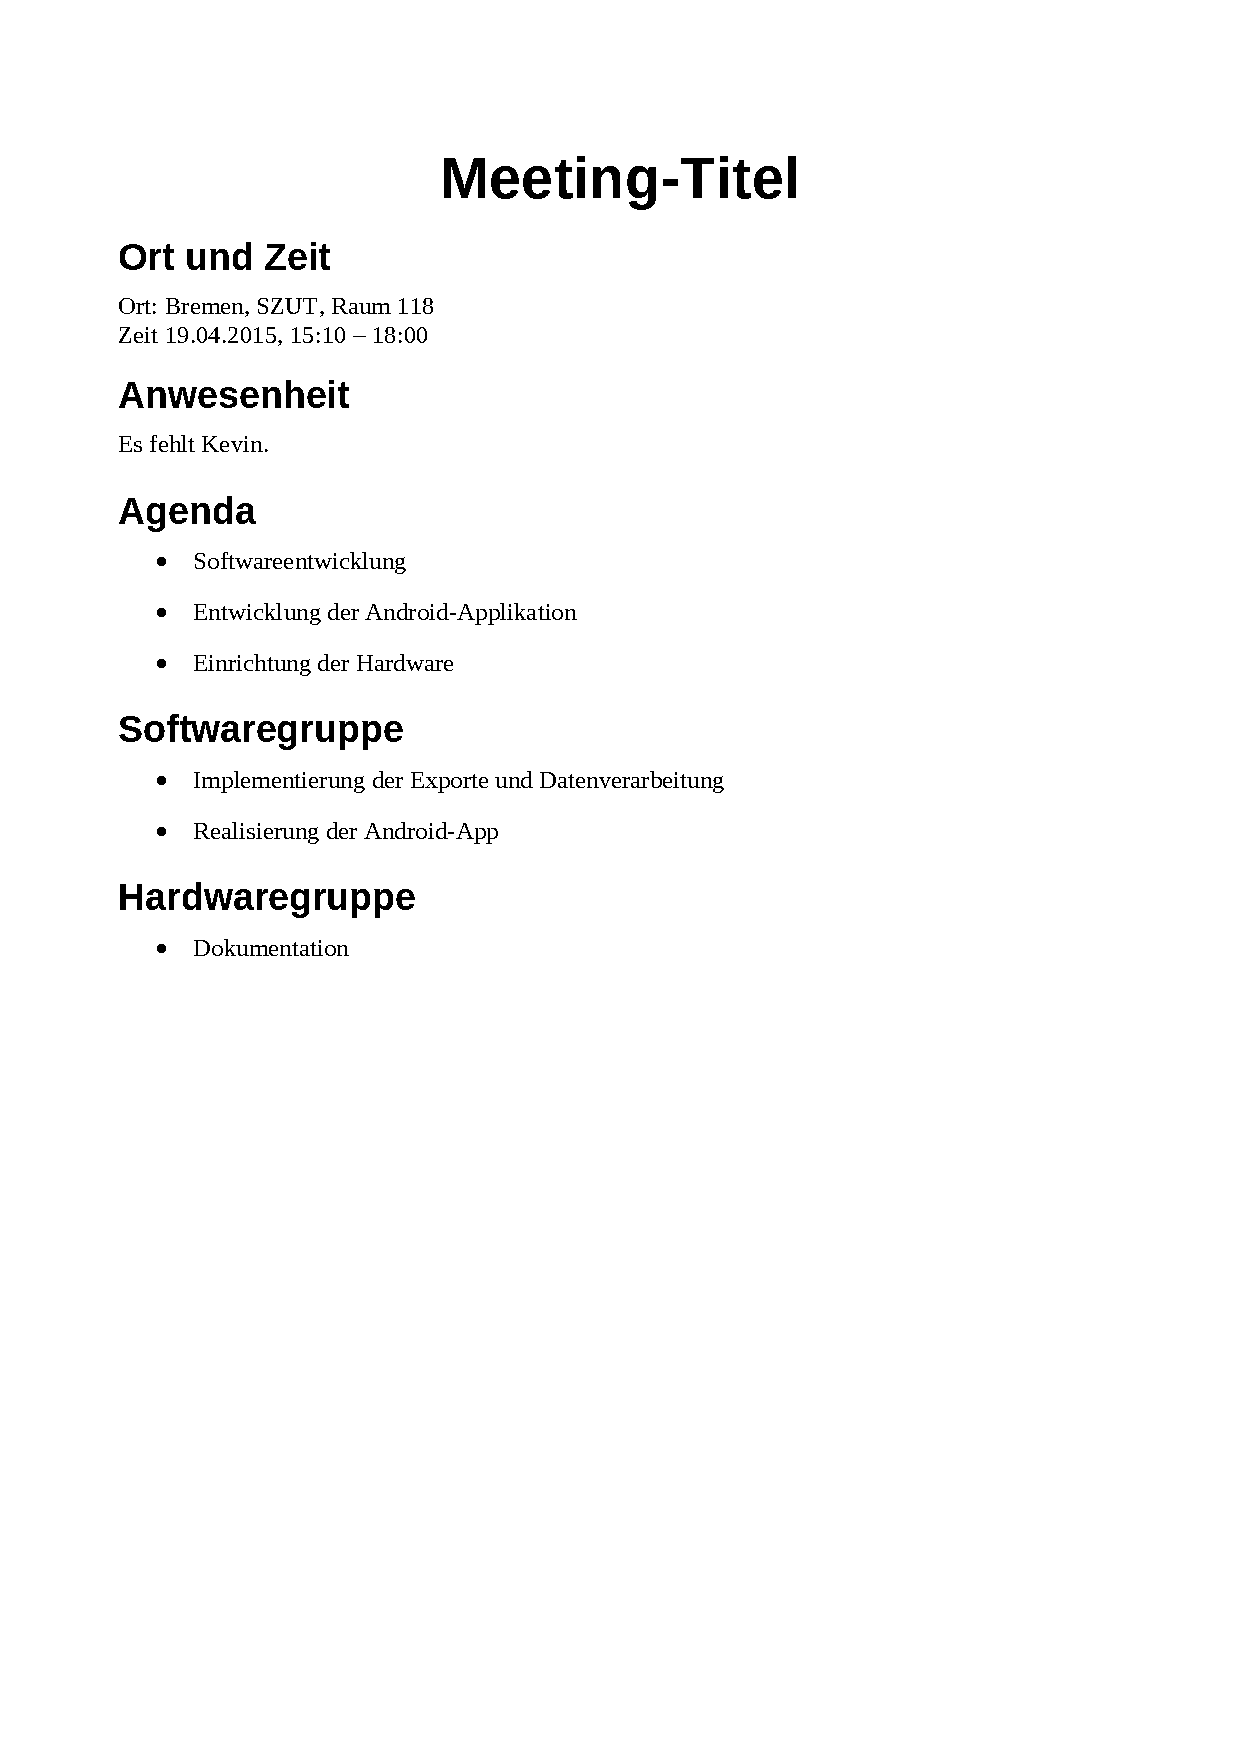
\includepdf{8_Anhang/Protokolle/150419_Meeting_Protokoll}%
\newpage
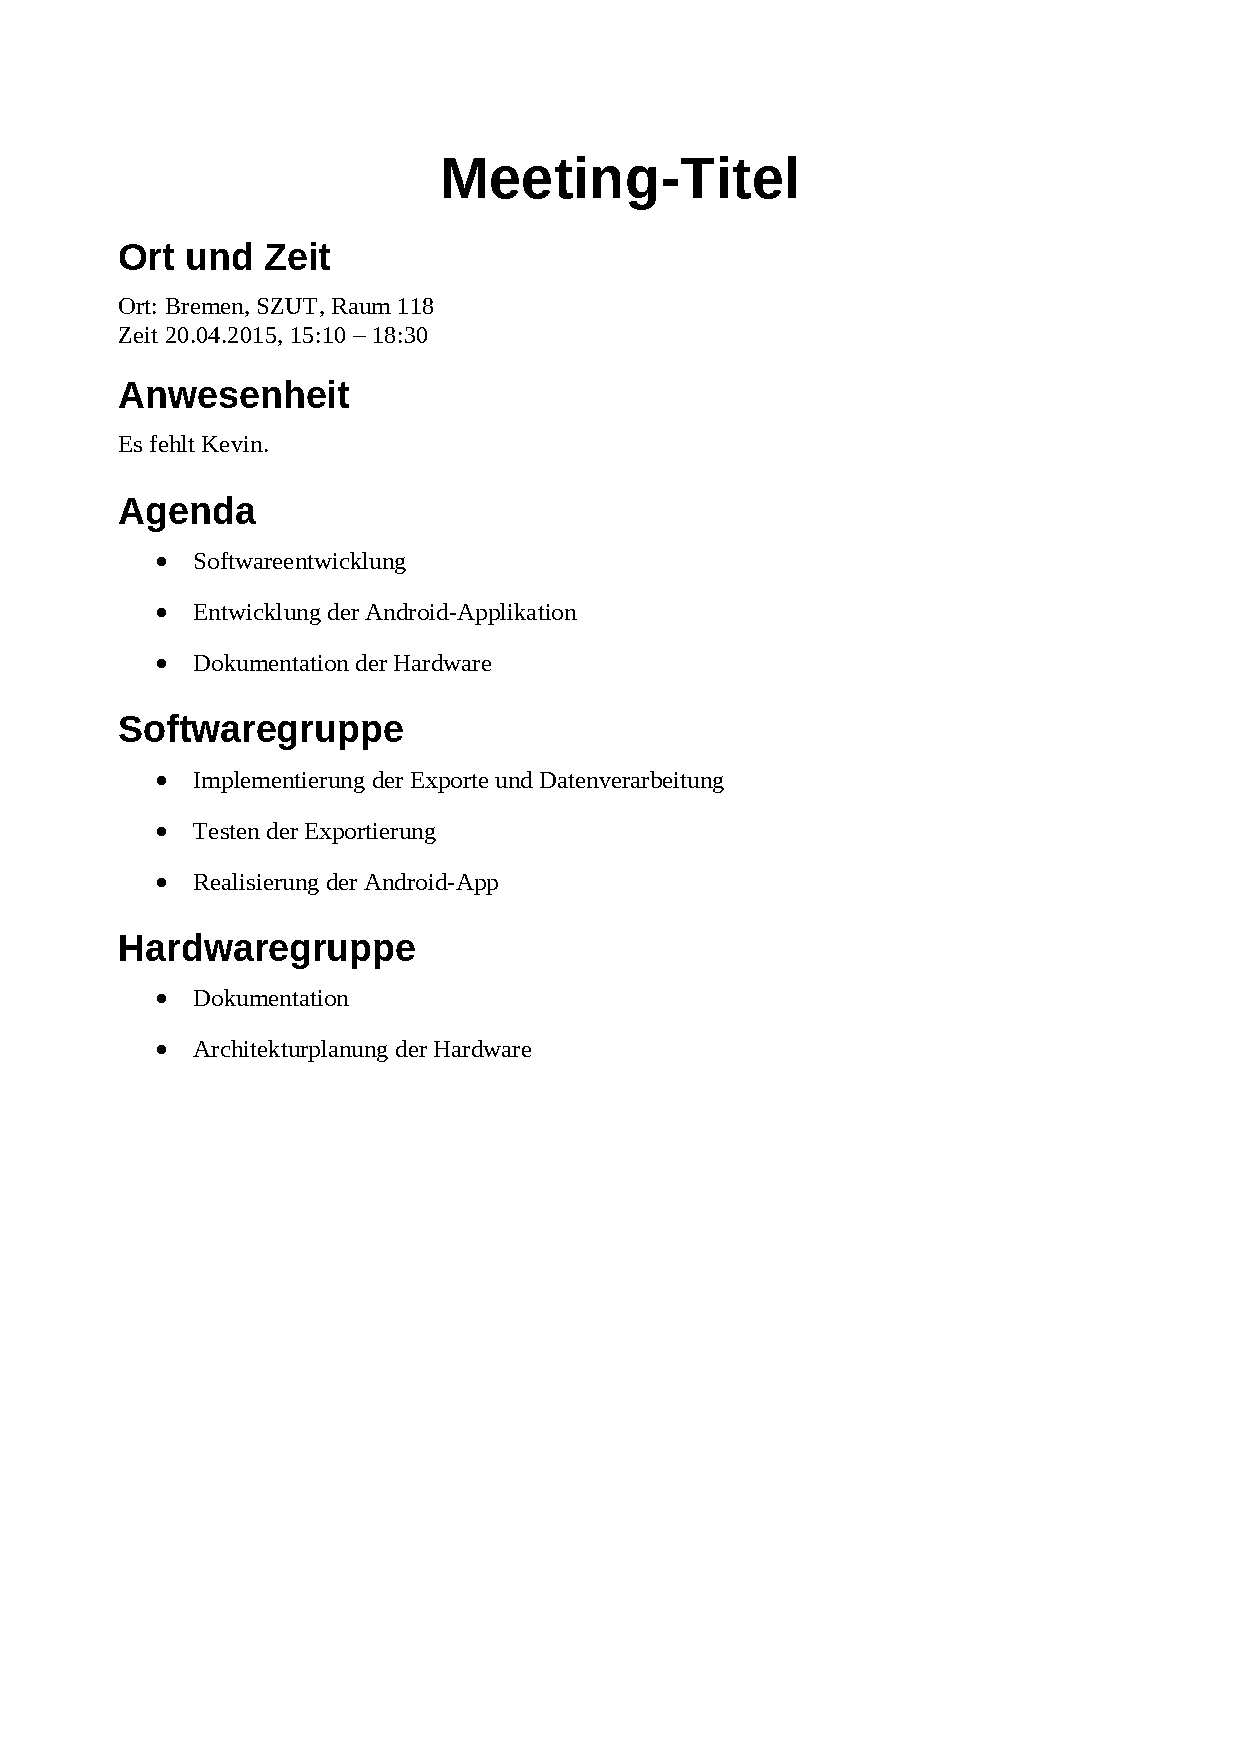
\includepdf{8_Anhang/Protokolle/150420_Meeting_Protokoll}%
\newpage
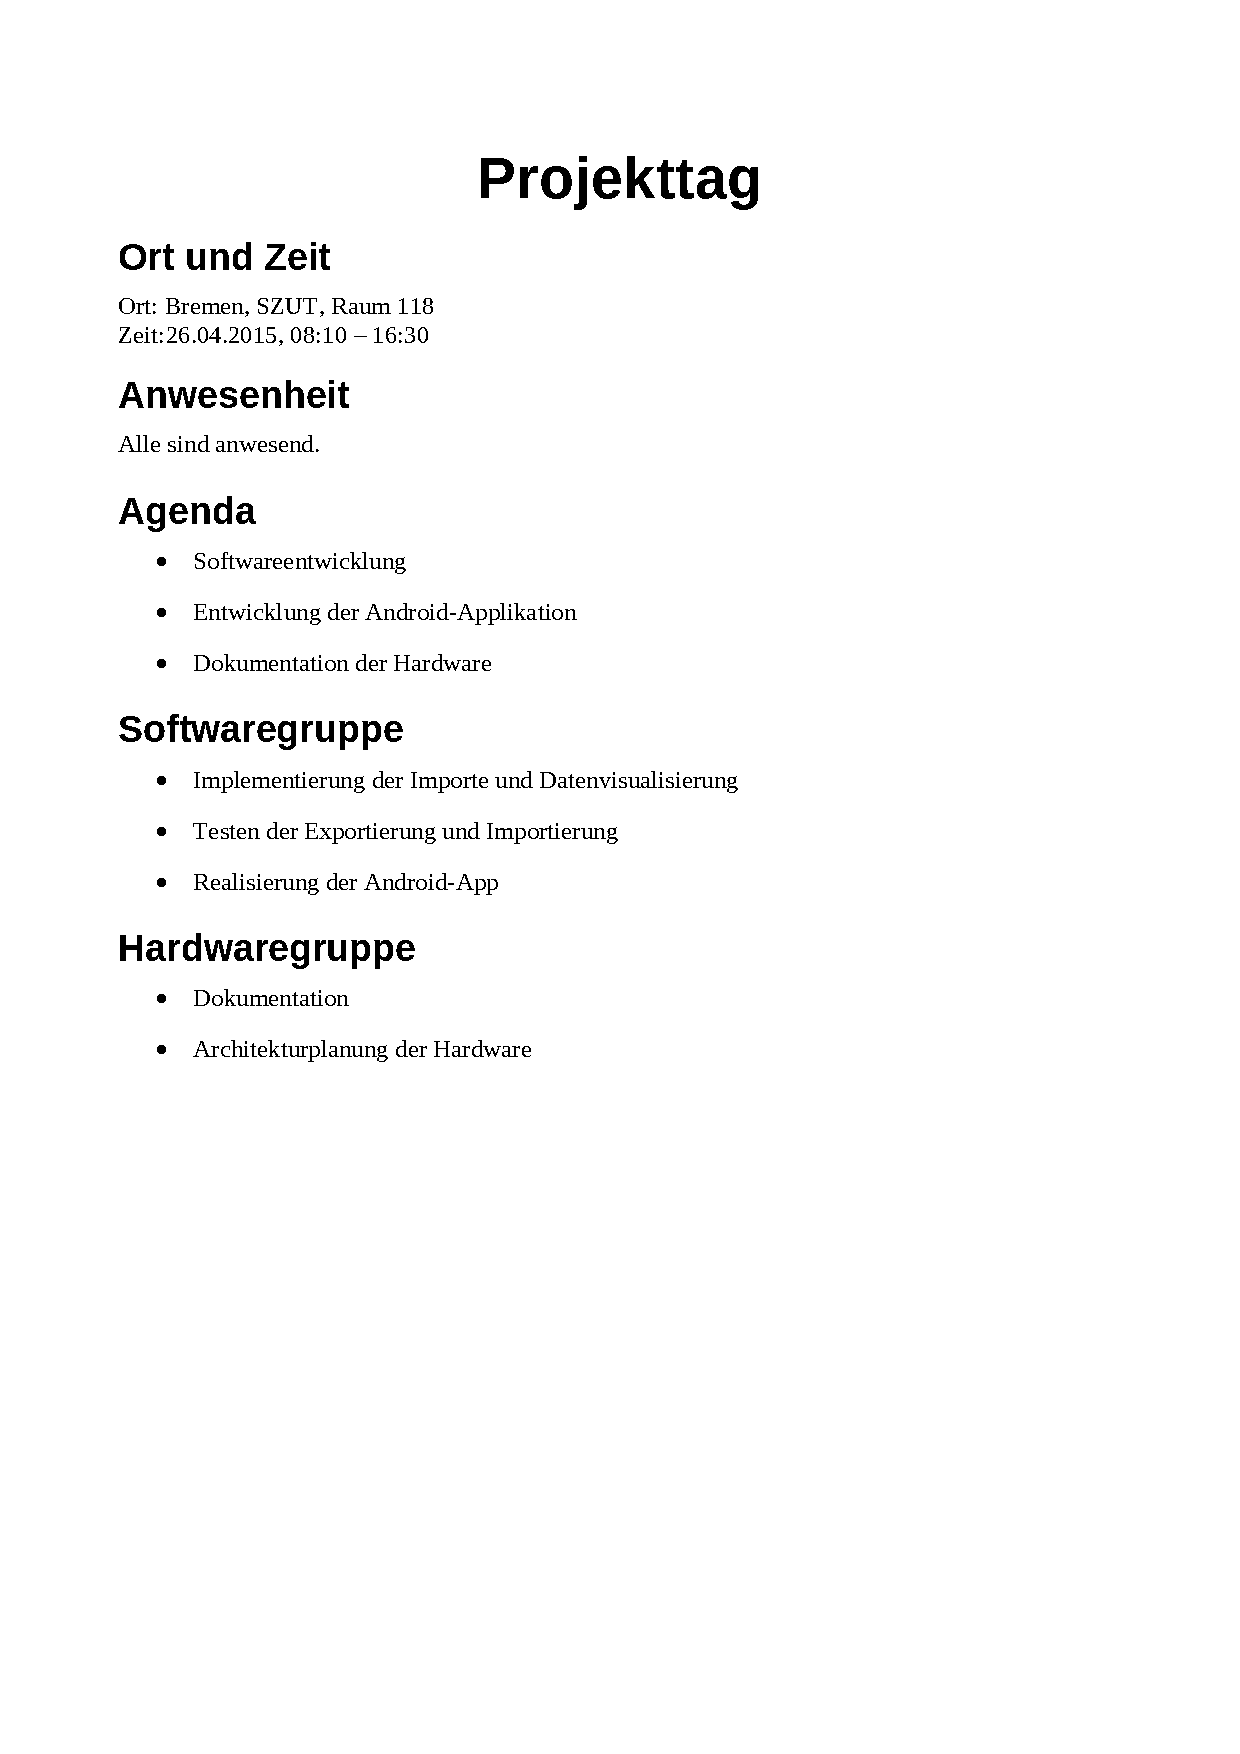
\includepdf{8_Anhang/Protokolle/150426_Meeting_Protokoll}%
\newpage
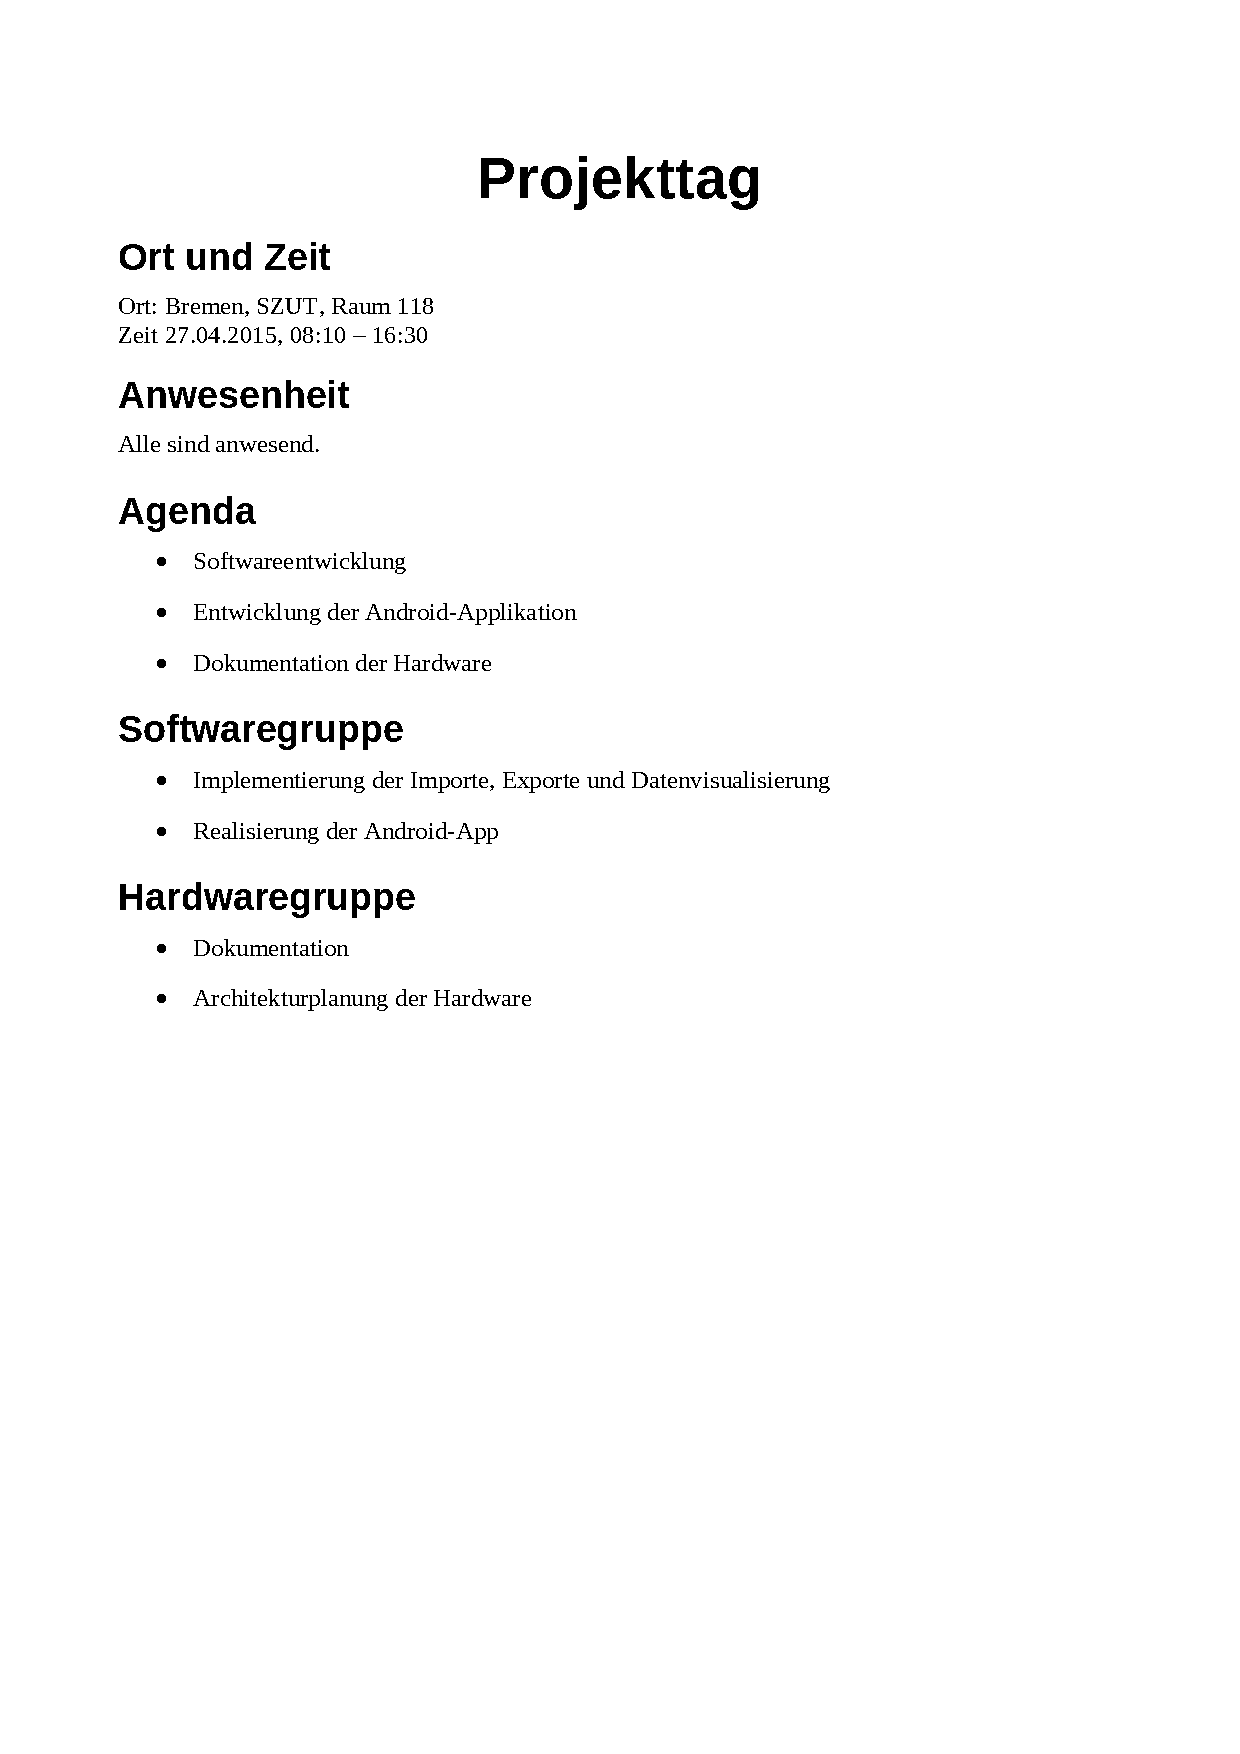
\includepdf{8_Anhang/Protokolle/150427_Meeting_Protokoll}%
\newpage
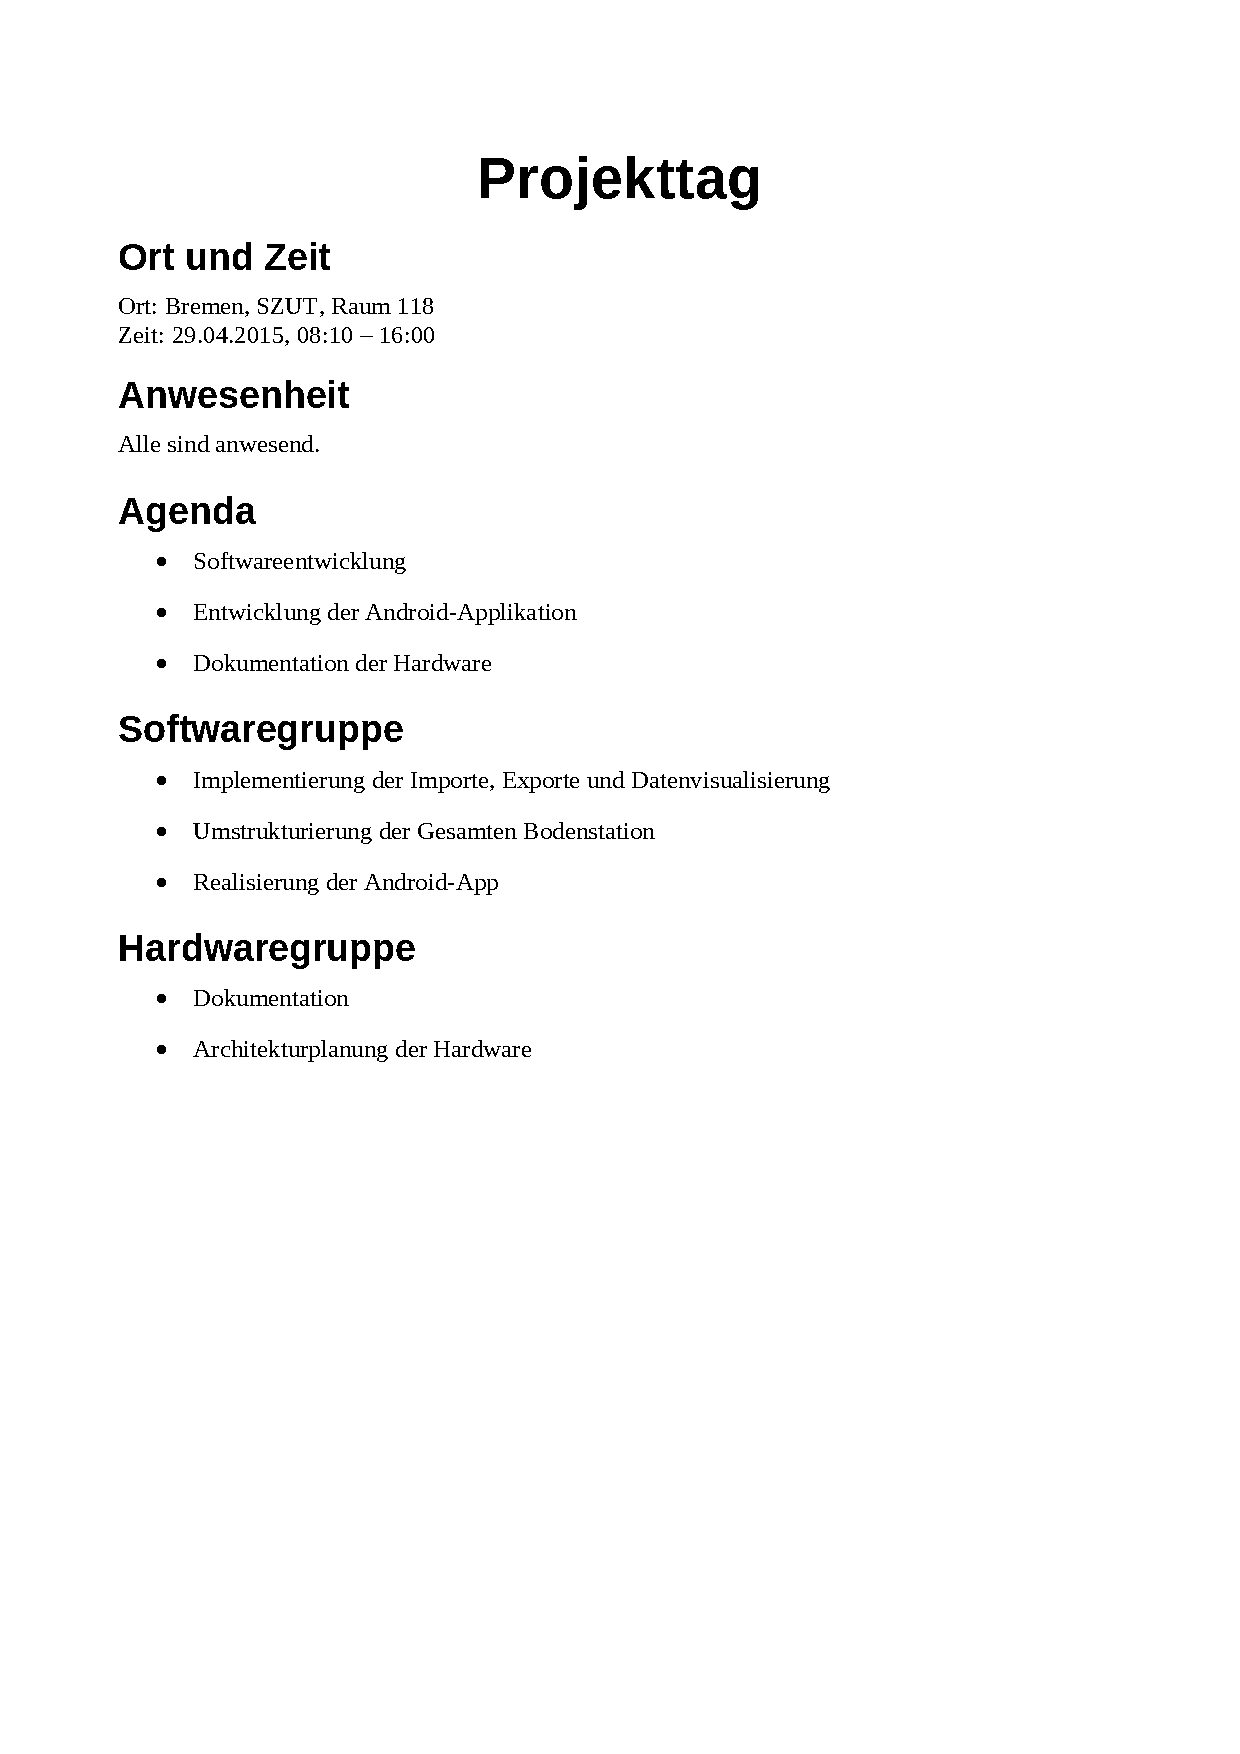
\includepdf{8_Anhang/Protokolle/150429_Meeting_Protokoll}%
\newpage
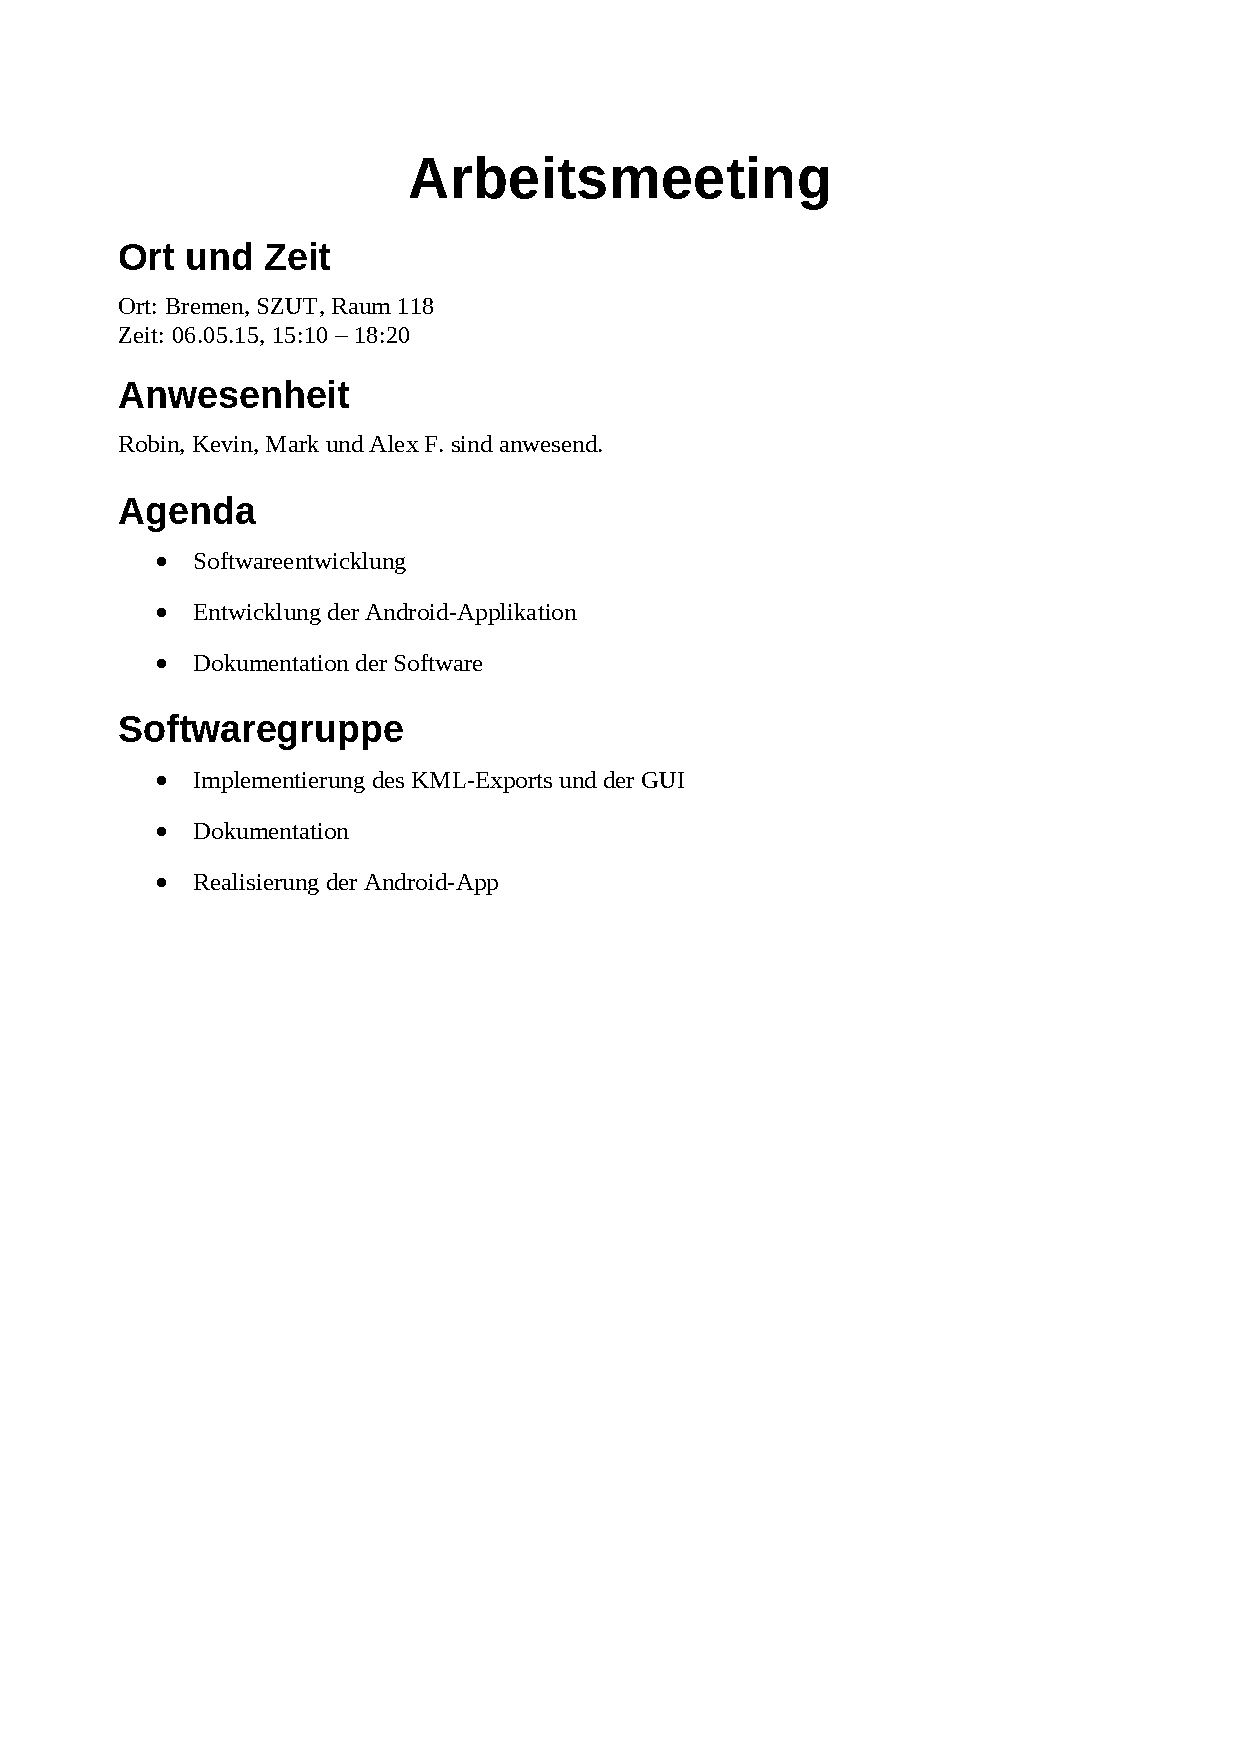
\includepdf{8_Anhang/Protokolle/150506_Meeting_Protokoll}%
\newpage
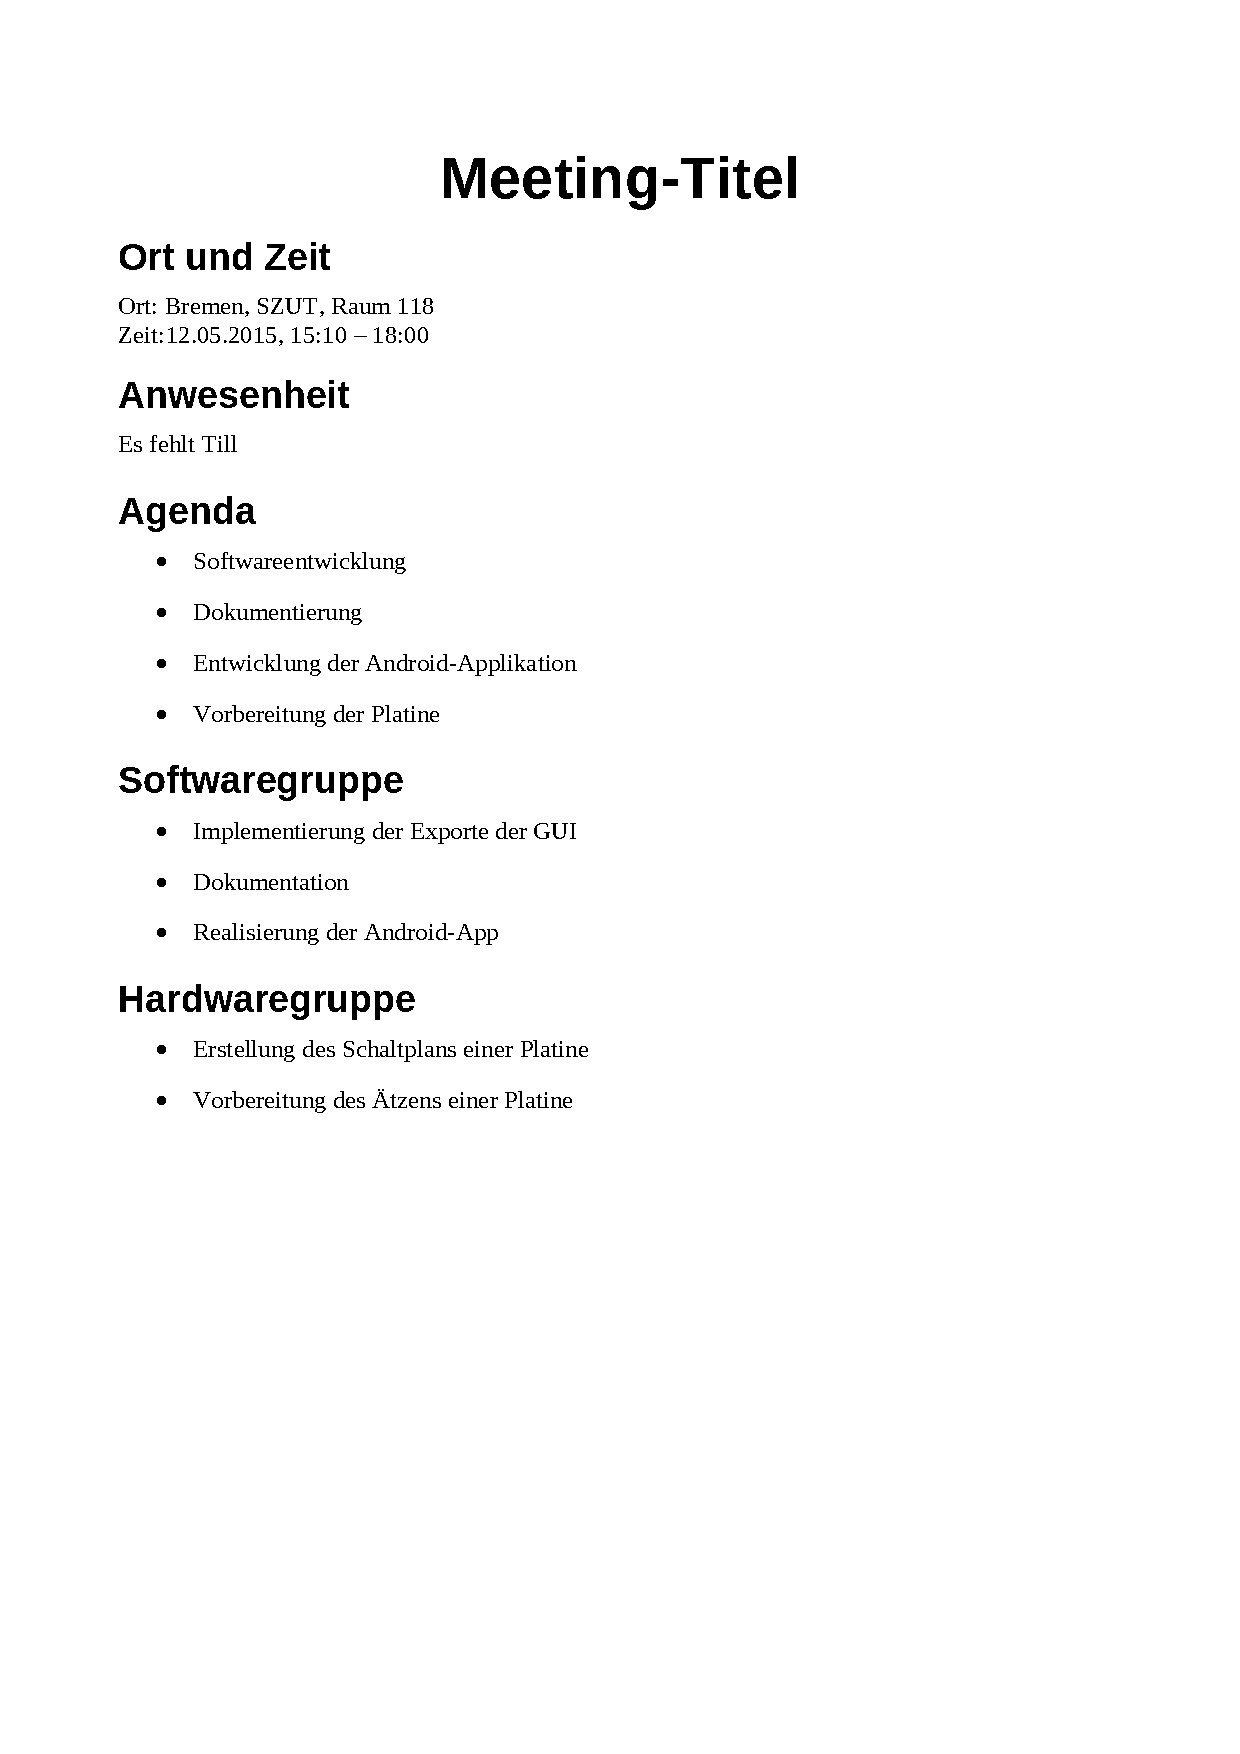
\includepdf{8_Anhang/Protokolle/150512_Meeting_Protokoll}%
\newpage
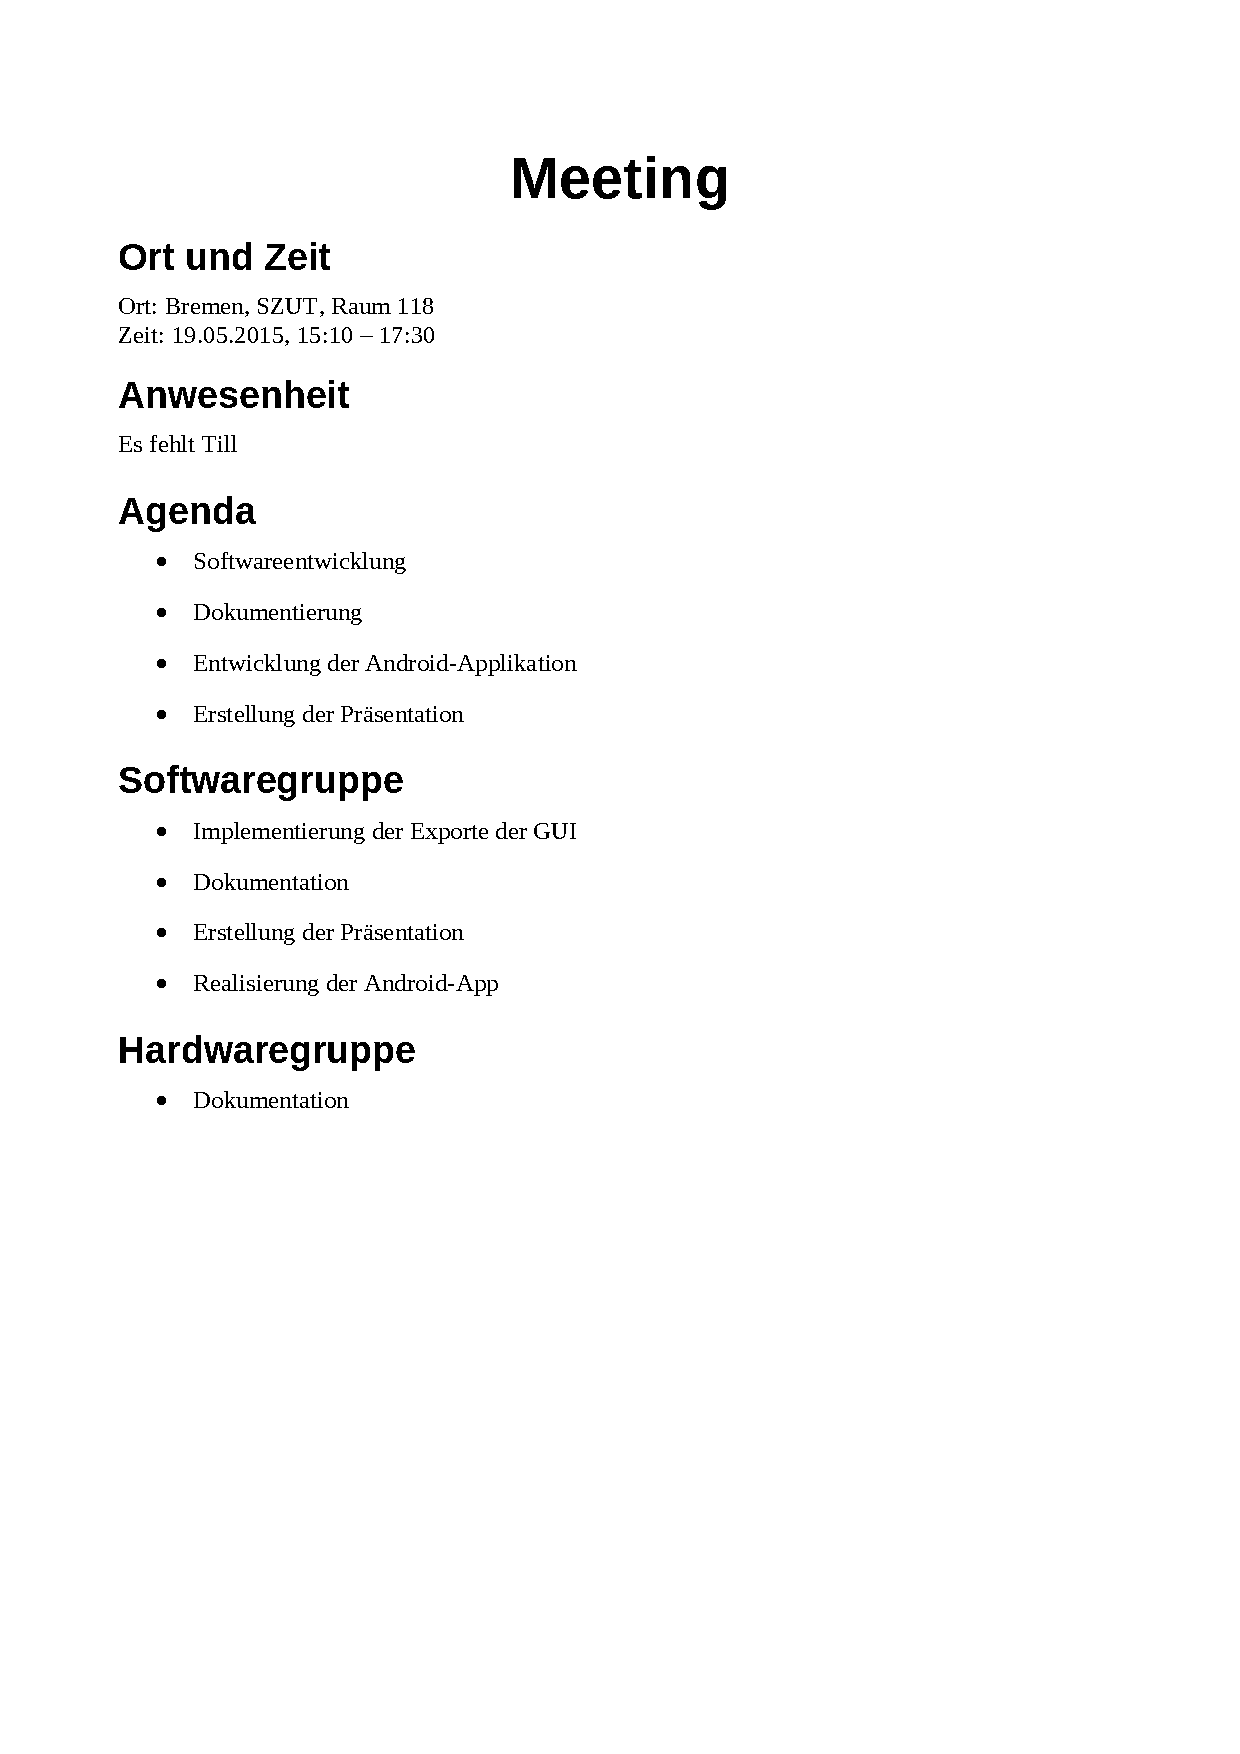
\includepdf{8_Anhang/Protokolle/150520_Meeting_Protokoll}%

\begin{comment}
0

{140921,141022,141202,141203,150106,150204,150210,150217,150303,150310,150317,150412,150419,150420,150426,150429,150506,150512,150520,150522} {

\foreach \i in {00, ..., 999999}%
    \edef\FileName{\i\_Meeting\_Protokoll}%     The % here are necessary to eliminate any
    \FileName%
    \IfFileExists{\FileName}{%  spurious spaces that may get inserted
    \includepdf[width=0.8\textwidth]{8_Anhang/Protokolle/\FileName}%
}%
}%

\end{comment}

